\chapter{Implementation}
This chapter will present how we implemented the protocols of chapter~\ref{chap:theory} on the board.
The figure~\ref{fig:os-path-generic} show the generic data flow in the operating system through the user and kernel spaces.
We will first detail the software part, with the OpenVPN and openSSH as the application, and OpenSSL as a cryptographic library on which both applications rely.
Then will come strongswan, a user-space abstraction layer giving access to IPSec and we will see how different it is from an OpenVPN implementation.
Lastly, the standard Linux cryptographic kernel modules and network drivers will be listed and briefly discussed.

Before closing the chapter, we will present the two main IPs to which the cryptographic operations will be offloaded and the associated drivers.


\begin{figure}[ht]
\center
\subfloat[\label{fig:os-path-generic-a}Generic]{%
	\Large
	\resizebox{.4\linewidth}{!}{%
	% Graphic for TeX using PGF
% Title: /home/para/documents/polytech2015/MA2/Master_thesis/master_thesis/os-path-generic.dia
% Creator: Dia v0.97.3
% CreationDate: Mon May 18 19:58:25 2015
% For: para
% \usepackage{tikz}
% The following commands are not supported in PSTricks at present
% We define them conditionally, so when they are implemented,
% this pgf file will use them.
\ifx\du\undefined
  \newlength{\du}
\fi
\setlength{\du}{15\unitlength}
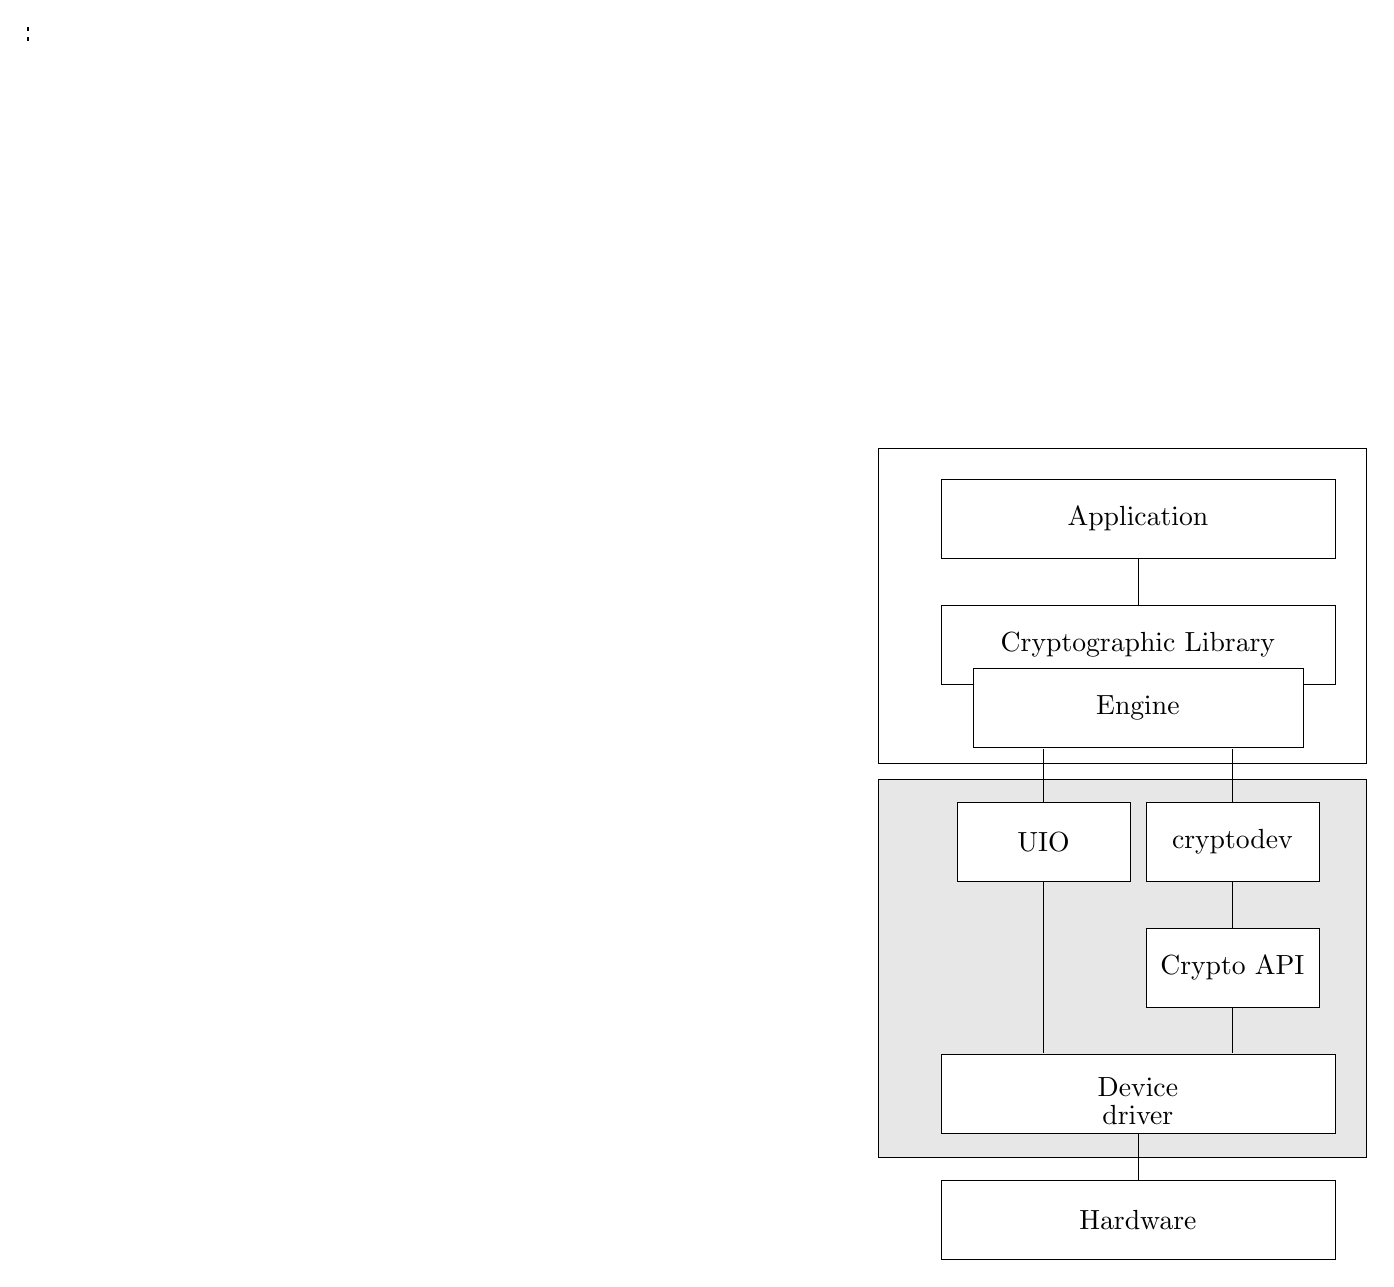
\begin{tikzpicture}
\pgftransformxscale{1.000000}
\pgftransformyscale{-1.000000}
\definecolor{dialinecolor}{rgb}{0.000000, 0.000000, 0.000000}
\pgfsetstrokecolor{dialinecolor}
\definecolor{dialinecolor}{rgb}{1.000000, 1.000000, 1.000000}
\pgfsetfillcolor{dialinecolor}
\pgfsetlinewidth{0.050000\du}
\pgfsetdash{}{0pt}
\pgfsetdash{}{0pt}
\pgfsetmiterjoin
\definecolor{dialinecolor}{rgb}{1.000000, 1.000000, 1.000000}
\pgfsetfillcolor{dialinecolor}
\fill (11.200000\du,5.600000\du)--(11.200000\du,9.600000\du)--(17.400000\du,9.600000\du)--(17.400000\du,5.600000\du)--cycle;
\definecolor{dialinecolor}{rgb}{0.000000, 0.000000, 0.000000}
\pgfsetstrokecolor{dialinecolor}
\draw (11.200000\du,5.600000\du)--(11.200000\du,9.600000\du)--(17.400000\du,9.600000\du)--(17.400000\du,5.600000\du)--cycle;
\pgfsetlinewidth{0.050000\du}
\pgfsetdash{}{0pt}
\pgfsetdash{}{0pt}
\pgfsetmiterjoin
\definecolor{dialinecolor}{rgb}{0.905882, 0.905882, 0.905882}
\pgfsetfillcolor{dialinecolor}
\fill (11.200000\du,9.800000\du)--(11.200000\du,14.600000\du)--(17.400000\du,14.600000\du)--(17.400000\du,9.800000\du)--cycle;
\definecolor{dialinecolor}{rgb}{0.000000, 0.000000, 0.000000}
\pgfsetstrokecolor{dialinecolor}
\draw (11.200000\du,9.800000\du)--(11.200000\du,14.600000\du)--(17.400000\du,14.600000\du)--(17.400000\du,9.800000\du)--cycle;
\pgfsetlinewidth{0.000000\du}
\pgfsetdash{}{0pt}
\pgfsetmiterjoin
\pgfsetroundcap
\definecolor{dialinecolor}{rgb}{0.000000, 0.000000, 0.000000}
\pgfsetfillcolor{dialinecolor}
\pgfpathmoveto{\pgfpoint{11.385372\du}{8.406740\du}}
\pgfpathlineto{\pgfpoint{11.392021\du}{8.357779\du}}
\pgfpathlineto{\pgfpoint{11.600318\du}{8.366119\du}}
\pgfpathcurveto{\pgfpoint{11.623347\du}{8.361767\du}}{\pgfpoint{11.642539\du}{8.358140\du}}{\pgfpoint{11.661731\du}{8.354513\du}}
\pgfpathcurveto{\pgfpoint{11.671795\du}{8.344661\du}}{\pgfpoint{11.678957\du}{8.319455\du}}{\pgfpoint{11.680831\du}{8.287297\du}}
\pgfpathcurveto{\pgfpoint{11.677204\du}{8.268106\du}}{\pgfpoint{11.669739\du}{8.249640\du}}{\pgfpoint{11.653872\du}{8.228786\du}}
\pgfpathcurveto{\pgfpoint{11.642569\du}{8.211045\du}}{\pgfpoint{11.625039\du}{8.202432\du}}{\pgfpoint{11.602009\du}{8.206784\du}}
\pgfpathlineto{\pgfpoint{11.393713\du}{8.198443\du}}
\pgfpathlineto{\pgfpoint{11.387910\du}{8.167737\du}}
\pgfpathlineto{\pgfpoint{11.596206\du}{8.176077\du}}
\pgfpathcurveto{\pgfpoint{11.638428\du}{8.168098\du}}{\pgfpoint{11.665085\du}{8.182938\du}}{\pgfpoint{11.681677\du}{8.207630\du}}
\pgfpathcurveto{\pgfpoint{11.705221\du}{8.227033\du}}{\pgfpoint{11.714137\du}{8.253176\du}}{\pgfpoint{11.711538\du}{8.281495\du}}
\pgfpathcurveto{\pgfpoint{11.708002\du}{8.325892\du}}{\pgfpoint{11.698451\du}{8.359500\du}}{\pgfpoint{11.682887\du}{8.382318\du}}
\pgfpathcurveto{\pgfpoint{11.665871\du}{8.397460\du}}{\pgfpoint{11.635890\du}{8.407101\du}}{\pgfpoint{11.593669\du}{8.415080\du}}
\pgfpathlineto{\pgfpoint{11.385372\du}{8.406740\du}}
\pgfusepath{fill}
\definecolor{dialinecolor}{rgb}{0.000000, 0.000000, 0.000000}
\pgfsetfillcolor{dialinecolor}
\pgfpathmoveto{\pgfpoint{11.483081\du}{7.935080\du}}
\pgfpathlineto{\pgfpoint{11.516689\du}{7.944630\du}}
\pgfpathcurveto{\pgfpoint{11.518865\du}{7.956145\du}}{\pgfpoint{11.521041\du}{7.967660\du}}{\pgfpoint{11.522492\du}{7.975337\du}}
\pgfpathcurveto{\pgfpoint{11.516991\du}{7.988303\du}}{\pgfpoint{11.508378\du}{8.005832\du}}{\pgfpoint{11.500490\du}{8.027200\du}}
\pgfpathcurveto{\pgfpoint{11.502666\du}{8.038714\du}}{\pgfpoint{11.512519\du}{8.048779\du}}{\pgfpoint{11.521646\du}{8.055005\du}}
\pgfpathcurveto{\pgfpoint{11.523822\du}{8.066520\du}}{\pgfpoint{11.532224\du}{8.068907\du}}{\pgfpoint{11.539901\du}{8.067456\du}}
\pgfpathcurveto{\pgfpoint{11.551416\du}{8.065280\du}}{\pgfpoint{11.562931\du}{8.063104\du}}{\pgfpoint{11.570607\du}{8.061653\du}}
\pgfpathcurveto{\pgfpoint{11.569156\du}{8.053977\du}}{\pgfpoint{11.573932\du}{8.037173\du}}{\pgfpoint{11.577256\du}{8.012692\du}}
\pgfpathlineto{\pgfpoint{11.574355\du}{7.997339\du}}
\pgfpathcurveto{\pgfpoint{11.584419\du}{7.987486\du}}{\pgfpoint{11.593758\du}{7.973795\du}}{\pgfpoint{11.599258\du}{7.960830\du}}
\pgfpathcurveto{\pgfpoint{11.609322\du}{7.950977\du}}{\pgfpoint{11.623225\du}{7.940399\du}}{\pgfpoint{11.642416\du}{7.936772\du}}
\pgfpathcurveto{\pgfpoint{11.667622\du}{7.943935\du}}{\pgfpoint{11.681313\du}{7.953273\du}}{\pgfpoint{11.694279\du}{7.958774\du}}
\pgfpathcurveto{\pgfpoint{11.704132\du}{7.968838\du}}{\pgfpoint{11.708484\du}{7.991868\du}}{\pgfpoint{11.705885\du}{8.020187\du}}
\pgfpathcurveto{\pgfpoint{11.710237\du}{8.043217\du}}{\pgfpoint{11.713139\du}{8.058570\du}}{\pgfpoint{11.714589\du}{8.066247\du}}
\pgfpathcurveto{\pgfpoint{11.716765\du}{8.077762\du}}{\pgfpoint{11.711990\du}{8.094566\du}}{\pgfpoint{11.707940\du}{8.115208\du}}
\pgfpathlineto{\pgfpoint{11.658979\du}{8.108559\du}}
\pgfpathcurveto{\pgfpoint{11.680558\du}{8.096530\du}}{\pgfpoint{11.686059\du}{8.083565\du}}{\pgfpoint{11.683883\du}{8.072050\du}}
\pgfpathcurveto{\pgfpoint{11.682432\du}{8.064373\du}}{\pgfpoint{11.679531\du}{8.049020\du}}{\pgfpoint{11.675178\du}{8.025990\du}}
\pgfpathcurveto{\pgfpoint{11.685243\du}{8.016137\du}}{\pgfpoint{11.686905\du}{8.003897\du}}{\pgfpoint{11.684729\du}{7.992382\du}}
\pgfpathcurveto{\pgfpoint{11.673425\du}{7.974641\du}}{\pgfpoint{11.659734\du}{7.965302\du}}{\pgfpoint{11.648219\du}{7.967478\du}}
\pgfpathcurveto{\pgfpoint{11.640543\du}{7.968929\du}}{\pgfpoint{11.634317\du}{7.978056\du}}{\pgfpoint{11.635767\du}{7.985733\du}}
\pgfpathcurveto{\pgfpoint{11.628091\du}{7.987184\du}}{\pgfpoint{11.618752\du}{8.000875\du}}{\pgfpoint{11.610864\du}{8.022243\du}}
\pgfpathlineto{\pgfpoint{11.598412\du}{8.040497\du}}
\pgfpathcurveto{\pgfpoint{11.604215\du}{8.071204\du}}{\pgfpoint{11.603278\du}{8.087282\du}}{\pgfpoint{11.591763\du}{8.089458\du}}
\pgfpathcurveto{\pgfpoint{11.572572\du}{8.093085\du}}{\pgfpoint{11.553380\du}{8.096712\du}}{\pgfpoint{11.530350\du}{8.101064\du}}
\pgfpathcurveto{\pgfpoint{11.522674\du}{8.102515\du}}{\pgfpoint{11.509708\du}{8.097015\du}}{\pgfpoint{11.493841\du}{8.076161\du}}
\pgfpathcurveto{\pgfpoint{11.482537\du}{8.058420\du}}{\pgfpoint{11.471234\du}{8.040679\du}}{\pgfpoint{11.466882\du}{8.017649\du}}
\pgfpathcurveto{\pgfpoint{11.476946\du}{8.007797\du}}{\pgfpoint{11.478608\du}{7.995556\du}}{\pgfpoint{11.476432\du}{7.984041\du}}
\pgfpathcurveto{\pgfpoint{11.472805\du}{7.964850\du}}{\pgfpoint{11.477580\du}{7.948046\du}}{\pgfpoint{11.483081\du}{7.935080\du}}
\pgfpathlineto{\pgfpoint{11.483081\du}{7.935080\du}}
\pgfusepath{fill}
\definecolor{dialinecolor}{rgb}{0.000000, 0.000000, 0.000000}
\pgfsetfillcolor{dialinecolor}
\pgfpathmoveto{\pgfpoint{11.586140\du}{7.681056\du}}
\pgfpathlineto{\pgfpoint{11.601493\du}{7.678154\du}}
\pgfpathlineto{\pgfpoint{11.602703\du}{7.852843\du}}
\pgfpathcurveto{\pgfpoint{11.633410\du}{7.847040\du}}{\pgfpoint{11.655714\du}{7.838850\du}}{\pgfpoint{11.661215\du}{7.825884\du}}
\pgfpathcurveto{\pgfpoint{11.671279\du}{7.816031\du}}{\pgfpoint{11.679892\du}{7.798502\du}}{\pgfpoint{11.683217\du}{7.774021\du}}
\pgfpathcurveto{\pgfpoint{11.681766\du}{7.766345\du}}{\pgfpoint{11.679590\du}{7.754830\du}}{\pgfpoint{11.677414\du}{7.743315\du}}
\pgfpathcurveto{\pgfpoint{11.681463\du}{7.722672\du}}{\pgfpoint{11.676386\du}{7.695804\du}}{\pgfpoint{11.662906\du}{7.666548\du}}
\pgfpathlineto{\pgfpoint{11.696514\du}{7.676099\du}}
\pgfpathcurveto{\pgfpoint{11.708543\du}{7.697678\du}}{\pgfpoint{11.712170\du}{7.716869\du}}{\pgfpoint{11.708120\du}{7.737512\du}}
\pgfpathcurveto{\pgfpoint{11.710296\du}{7.749027\du}}{\pgfpoint{11.712472\du}{7.760542\du}}{\pgfpoint{11.713923\du}{7.768218\du}}
\pgfpathcurveto{\pgfpoint{11.710387\du}{7.812616\du}}{\pgfpoint{11.700112\du}{7.842385\du}}{\pgfpoint{11.682371\du}{7.853689\du}}
\pgfpathcurveto{\pgfpoint{11.657679\du}{7.870281\du}}{\pgfpoint{11.623859\du}{7.880648\du}}{\pgfpoint{11.593153\du}{7.886451\du}}
\pgfpathcurveto{\pgfpoint{11.553319\du}{7.886028\du}}{\pgfpoint{11.523549\du}{7.875752\du}}{\pgfpoint{11.507682\du}{7.854899\du}}
\pgfpathcurveto{\pgfpoint{11.484864\du}{7.839334\du}}{\pgfpoint{11.475222\du}{7.809353\du}}{\pgfpoint{11.474920\du}{7.765681\du}}
\pgfpathcurveto{\pgfpoint{11.469842\du}{7.738812\du}}{\pgfpoint{11.484682\du}{7.712156\du}}{\pgfpoint{11.509374\du}{7.695563\du}}
\pgfpathcurveto{\pgfpoint{11.530953\du}{7.683534\du}}{\pgfpoint{11.557821\du}{7.678457\du}}{\pgfpoint{11.586140\du}{7.681056\du}}
\pgfpathlineto{\pgfpoint{11.586140\du}{7.681056\du}}
\pgfusepath{fill}
\definecolor{dialinecolor}{rgb}{1.000000, 1.000000, 1.000000}
\pgfsetfillcolor{dialinecolor}
\pgfpathmoveto{\pgfpoint{11.561237\du}{7.717565\du}}
\pgfpathcurveto{\pgfpoint{11.553560\du}{7.719016\du}}{\pgfpoint{11.543496\du}{7.728869\du}}{\pgfpoint{11.533432\du}{7.738721\du}}
\pgfpathcurveto{\pgfpoint{11.516416\du}{7.753863\du}}{\pgfpoint{11.507077\du}{7.767554\du}}{\pgfpoint{11.508528\du}{7.775231\du}}
\pgfpathcurveto{\pgfpoint{11.505204\du}{7.799711\du}}{\pgfpoint{11.508830\du}{7.818903\du}}{\pgfpoint{11.520134\du}{7.836644\du}}
\pgfpathcurveto{\pgfpoint{11.533825\du}{7.845983\du}}{\pgfpoint{11.549904\du}{7.846919\du}}{\pgfpoint{11.569095\du}{7.843293\du}}
\pgfusepath{fill}
\definecolor{dialinecolor}{rgb}{0.000000, 0.000000, 0.000000}
\pgfsetfillcolor{dialinecolor}
\pgfpathmoveto{\pgfpoint{11.520102\du}{7.478865\du}}
\pgfpathcurveto{\pgfpoint{11.522278\du}{7.490379\du}}{\pgfpoint{11.523004\du}{7.494218\du}}{\pgfpoint{11.523004\du}{7.494218\du}}
\pgfpathcurveto{\pgfpoint{11.515327\du}{7.495669\du}}{\pgfpoint{11.509101\du}{7.504796\du}}{\pgfpoint{11.510552\du}{7.512473\du}}
\pgfpathcurveto{\pgfpoint{11.507227\du}{7.536953\du}}{\pgfpoint{11.513967\du}{7.551581\du}}{\pgfpoint{11.534610\du}{7.555631\du}}
\pgfpathcurveto{\pgfpoint{11.548301\du}{7.564970\du}}{\pgfpoint{11.573507\du}{7.572132\du}}{\pgfpoint{11.601825\du}{7.574731\du}}
\pgfpathlineto{\pgfpoint{11.712200\du}{7.569774\du}}
\pgfpathlineto{\pgfpoint{11.705551\du}{7.618736\du}}
\pgfpathlineto{\pgfpoint{11.466548\du}{7.616198\du}}
\pgfpathlineto{\pgfpoint{11.473197\du}{7.567237\du}}
\pgfpathlineto{\pgfpoint{11.522158\du}{7.573885\du}}
\pgfpathcurveto{\pgfpoint{11.501515\du}{7.569836\du}}{\pgfpoint{11.487824\du}{7.560497\du}}{\pgfpoint{11.485648\du}{7.548982\du}}
\pgfpathcurveto{\pgfpoint{11.474345\du}{7.531241\du}}{\pgfpoint{11.470718\du}{7.512050\du}}{\pgfpoint{11.474042\du}{7.487569\du}}
\pgfpathcurveto{\pgfpoint{11.474042\du}{7.487569\du}}{\pgfpoint{11.473317\du}{7.483731\du}}{\pgfpoint{11.471141\du}{7.472216\du}}
\pgfpathlineto{\pgfpoint{11.520102\du}{7.478865\du}}
\pgfusepath{fill}
\definecolor{dialinecolor}{rgb}{0.000000, 0.000000, 0.000000}
\pgfsetstrokecolor{dialinecolor}
\pgfpathmoveto{\pgfpoint{11.385372\du}{8.406740\du}}
\pgfpathlineto{\pgfpoint{11.392021\du}{8.357779\du}}
\pgfpathlineto{\pgfpoint{11.600318\du}{8.366119\du}}
\pgfpathcurveto{\pgfpoint{11.623347\du}{8.361767\du}}{\pgfpoint{11.642539\du}{8.358140\du}}{\pgfpoint{11.661731\du}{8.354513\du}}
\pgfpathcurveto{\pgfpoint{11.671795\du}{8.344661\du}}{\pgfpoint{11.678957\du}{8.319455\du}}{\pgfpoint{11.680831\du}{8.287297\du}}
\pgfpathcurveto{\pgfpoint{11.677204\du}{8.268106\du}}{\pgfpoint{11.669739\du}{8.249640\du}}{\pgfpoint{11.653872\du}{8.228786\du}}
\pgfpathcurveto{\pgfpoint{11.642569\du}{8.211045\du}}{\pgfpoint{11.625039\du}{8.202432\du}}{\pgfpoint{11.602009\du}{8.206784\du}}
\pgfpathlineto{\pgfpoint{11.393713\du}{8.198443\du}}
\pgfpathlineto{\pgfpoint{11.387910\du}{8.167737\du}}
\pgfpathlineto{\pgfpoint{11.596206\du}{8.176077\du}}
\pgfpathcurveto{\pgfpoint{11.638428\du}{8.168098\du}}{\pgfpoint{11.665085\du}{8.182938\du}}{\pgfpoint{11.681677\du}{8.207630\du}}
\pgfpathcurveto{\pgfpoint{11.705221\du}{8.227033\du}}{\pgfpoint{11.714137\du}{8.253176\du}}{\pgfpoint{11.711538\du}{8.281495\du}}
\pgfpathcurveto{\pgfpoint{11.708002\du}{8.325892\du}}{\pgfpoint{11.698451\du}{8.359500\du}}{\pgfpoint{11.682887\du}{8.382318\du}}
\pgfpathcurveto{\pgfpoint{11.665871\du}{8.397460\du}}{\pgfpoint{11.635890\du}{8.407101\du}}{\pgfpoint{11.593669\du}{8.415080\du}}
\pgfpathlineto{\pgfpoint{11.385372\du}{8.406740\du}}
\pgfusepath{stroke}
\definecolor{dialinecolor}{rgb}{0.000000, 0.000000, 0.000000}
\pgfsetstrokecolor{dialinecolor}
\pgfpathmoveto{\pgfpoint{11.483081\du}{7.935080\du}}
\pgfpathlineto{\pgfpoint{11.516689\du}{7.944630\du}}
\pgfpathcurveto{\pgfpoint{11.518865\du}{7.956145\du}}{\pgfpoint{11.521041\du}{7.967660\du}}{\pgfpoint{11.522492\du}{7.975337\du}}
\pgfpathcurveto{\pgfpoint{11.516991\du}{7.988303\du}}{\pgfpoint{11.508378\du}{8.005832\du}}{\pgfpoint{11.500490\du}{8.027200\du}}
\pgfpathcurveto{\pgfpoint{11.502666\du}{8.038714\du}}{\pgfpoint{11.512519\du}{8.048779\du}}{\pgfpoint{11.521646\du}{8.055005\du}}
\pgfpathcurveto{\pgfpoint{11.523822\du}{8.066520\du}}{\pgfpoint{11.532224\du}{8.068907\du}}{\pgfpoint{11.539901\du}{8.067456\du}}
\pgfpathcurveto{\pgfpoint{11.551416\du}{8.065280\du}}{\pgfpoint{11.562931\du}{8.063104\du}}{\pgfpoint{11.570607\du}{8.061653\du}}
\pgfpathcurveto{\pgfpoint{11.569156\du}{8.053977\du}}{\pgfpoint{11.573932\du}{8.037173\du}}{\pgfpoint{11.577256\du}{8.012692\du}}
\pgfpathlineto{\pgfpoint{11.574355\du}{7.997339\du}}
\pgfpathcurveto{\pgfpoint{11.584419\du}{7.987486\du}}{\pgfpoint{11.593758\du}{7.973795\du}}{\pgfpoint{11.599258\du}{7.960830\du}}
\pgfpathcurveto{\pgfpoint{11.609322\du}{7.950977\du}}{\pgfpoint{11.623225\du}{7.940399\du}}{\pgfpoint{11.642416\du}{7.936772\du}}
\pgfpathcurveto{\pgfpoint{11.667622\du}{7.943935\du}}{\pgfpoint{11.681313\du}{7.953273\du}}{\pgfpoint{11.694279\du}{7.958774\du}}
\pgfpathcurveto{\pgfpoint{11.704132\du}{7.968838\du}}{\pgfpoint{11.708484\du}{7.991868\du}}{\pgfpoint{11.705885\du}{8.020187\du}}
\pgfpathcurveto{\pgfpoint{11.710237\du}{8.043217\du}}{\pgfpoint{11.713139\du}{8.058570\du}}{\pgfpoint{11.714589\du}{8.066247\du}}
\pgfpathcurveto{\pgfpoint{11.716765\du}{8.077762\du}}{\pgfpoint{11.711990\du}{8.094566\du}}{\pgfpoint{11.707940\du}{8.115208\du}}
\pgfpathlineto{\pgfpoint{11.658979\du}{8.108559\du}}
\pgfpathcurveto{\pgfpoint{11.680558\du}{8.096530\du}}{\pgfpoint{11.686059\du}{8.083565\du}}{\pgfpoint{11.683883\du}{8.072050\du}}
\pgfpathcurveto{\pgfpoint{11.682432\du}{8.064373\du}}{\pgfpoint{11.679531\du}{8.049020\du}}{\pgfpoint{11.675178\du}{8.025990\du}}
\pgfpathcurveto{\pgfpoint{11.685243\du}{8.016137\du}}{\pgfpoint{11.686905\du}{8.003897\du}}{\pgfpoint{11.684729\du}{7.992382\du}}
\pgfpathcurveto{\pgfpoint{11.673425\du}{7.974641\du}}{\pgfpoint{11.659734\du}{7.965302\du}}{\pgfpoint{11.648219\du}{7.967478\du}}
\pgfpathcurveto{\pgfpoint{11.640543\du}{7.968929\du}}{\pgfpoint{11.634317\du}{7.978056\du}}{\pgfpoint{11.635767\du}{7.985733\du}}
\pgfpathcurveto{\pgfpoint{11.628091\du}{7.987184\du}}{\pgfpoint{11.618752\du}{8.000875\du}}{\pgfpoint{11.610864\du}{8.022243\du}}
\pgfpathlineto{\pgfpoint{11.598412\du}{8.040497\du}}
\pgfpathcurveto{\pgfpoint{11.604215\du}{8.071204\du}}{\pgfpoint{11.603278\du}{8.087282\du}}{\pgfpoint{11.591763\du}{8.089458\du}}
\pgfpathcurveto{\pgfpoint{11.572572\du}{8.093085\du}}{\pgfpoint{11.553380\du}{8.096712\du}}{\pgfpoint{11.530350\du}{8.101064\du}}
\pgfpathcurveto{\pgfpoint{11.522674\du}{8.102515\du}}{\pgfpoint{11.509708\du}{8.097015\du}}{\pgfpoint{11.493841\du}{8.076161\du}}
\pgfpathcurveto{\pgfpoint{11.482537\du}{8.058420\du}}{\pgfpoint{11.471234\du}{8.040679\du}}{\pgfpoint{11.466882\du}{8.017649\du}}
\pgfpathcurveto{\pgfpoint{11.476946\du}{8.007797\du}}{\pgfpoint{11.478608\du}{7.995556\du}}{\pgfpoint{11.476432\du}{7.984041\du}}
\pgfpathcurveto{\pgfpoint{11.472805\du}{7.964850\du}}{\pgfpoint{11.477580\du}{7.948046\du}}{\pgfpoint{11.483081\du}{7.935080\du}}
\pgfpathlineto{\pgfpoint{11.483081\du}{7.935080\du}}
\pgfusepath{stroke}
\definecolor{dialinecolor}{rgb}{0.000000, 0.000000, 0.000000}
\pgfsetstrokecolor{dialinecolor}
\pgfpathmoveto{\pgfpoint{11.586140\du}{7.681056\du}}
\pgfpathlineto{\pgfpoint{11.601493\du}{7.678154\du}}
\pgfpathlineto{\pgfpoint{11.602703\du}{7.852843\du}}
\pgfpathcurveto{\pgfpoint{11.633410\du}{7.847040\du}}{\pgfpoint{11.655714\du}{7.838850\du}}{\pgfpoint{11.661215\du}{7.825884\du}}
\pgfpathcurveto{\pgfpoint{11.671279\du}{7.816031\du}}{\pgfpoint{11.679892\du}{7.798502\du}}{\pgfpoint{11.683217\du}{7.774021\du}}
\pgfpathcurveto{\pgfpoint{11.681766\du}{7.766345\du}}{\pgfpoint{11.679590\du}{7.754830\du}}{\pgfpoint{11.677414\du}{7.743315\du}}
\pgfpathcurveto{\pgfpoint{11.681463\du}{7.722672\du}}{\pgfpoint{11.676386\du}{7.695804\du}}{\pgfpoint{11.662906\du}{7.666548\du}}
\pgfpathlineto{\pgfpoint{11.696514\du}{7.676099\du}}
\pgfpathcurveto{\pgfpoint{11.708543\du}{7.697678\du}}{\pgfpoint{11.712170\du}{7.716869\du}}{\pgfpoint{11.708120\du}{7.737512\du}}
\pgfpathcurveto{\pgfpoint{11.710296\du}{7.749027\du}}{\pgfpoint{11.712472\du}{7.760542\du}}{\pgfpoint{11.713923\du}{7.768218\du}}
\pgfpathcurveto{\pgfpoint{11.710387\du}{7.812616\du}}{\pgfpoint{11.700112\du}{7.842385\du}}{\pgfpoint{11.682371\du}{7.853689\du}}
\pgfpathcurveto{\pgfpoint{11.657679\du}{7.870281\du}}{\pgfpoint{11.623859\du}{7.880648\du}}{\pgfpoint{11.593153\du}{7.886451\du}}
\pgfpathcurveto{\pgfpoint{11.553319\du}{7.886028\du}}{\pgfpoint{11.523549\du}{7.875752\du}}{\pgfpoint{11.507682\du}{7.854899\du}}
\pgfpathcurveto{\pgfpoint{11.484864\du}{7.839334\du}}{\pgfpoint{11.475222\du}{7.809353\du}}{\pgfpoint{11.474920\du}{7.765681\du}}
\pgfpathcurveto{\pgfpoint{11.469842\du}{7.738812\du}}{\pgfpoint{11.484682\du}{7.712156\du}}{\pgfpoint{11.509374\du}{7.695563\du}}
\pgfpathcurveto{\pgfpoint{11.530953\du}{7.683534\du}}{\pgfpoint{11.557821\du}{7.678457\du}}{\pgfpoint{11.586140\du}{7.681056\du}}
\pgfpathlineto{\pgfpoint{11.586140\du}{7.681056\du}}
\pgfusepath{stroke}
\definecolor{dialinecolor}{rgb}{0.000000, 0.000000, 0.000000}
\pgfsetstrokecolor{dialinecolor}
\pgfpathmoveto{\pgfpoint{11.561237\du}{7.717565\du}}
\pgfpathcurveto{\pgfpoint{11.553560\du}{7.719016\du}}{\pgfpoint{11.543496\du}{7.728869\du}}{\pgfpoint{11.533432\du}{7.738721\du}}
\pgfpathcurveto{\pgfpoint{11.516416\du}{7.753863\du}}{\pgfpoint{11.507077\du}{7.767554\du}}{\pgfpoint{11.508528\du}{7.775231\du}}
\pgfpathcurveto{\pgfpoint{11.505204\du}{7.799711\du}}{\pgfpoint{11.508830\du}{7.818903\du}}{\pgfpoint{11.520134\du}{7.836644\du}}
\pgfpathcurveto{\pgfpoint{11.533825\du}{7.845983\du}}{\pgfpoint{11.549904\du}{7.846919\du}}{\pgfpoint{11.569095\du}{7.843293\du}}
\pgfpathlineto{\pgfpoint{11.561237\du}{7.717565\du}}
\pgfusepath{stroke}
\definecolor{dialinecolor}{rgb}{0.000000, 0.000000, 0.000000}
\pgfsetstrokecolor{dialinecolor}
\pgfpathmoveto{\pgfpoint{11.520102\du}{7.478865\du}}
\pgfpathcurveto{\pgfpoint{11.522278\du}{7.490379\du}}{\pgfpoint{11.523004\du}{7.494218\du}}{\pgfpoint{11.523004\du}{7.494218\du}}
\pgfpathcurveto{\pgfpoint{11.515327\du}{7.495669\du}}{\pgfpoint{11.509101\du}{7.504796\du}}{\pgfpoint{11.510552\du}{7.512473\du}}
\pgfpathcurveto{\pgfpoint{11.507227\du}{7.536953\du}}{\pgfpoint{11.513967\du}{7.551581\du}}{\pgfpoint{11.534610\du}{7.555631\du}}
\pgfpathcurveto{\pgfpoint{11.548301\du}{7.564970\du}}{\pgfpoint{11.573507\du}{7.572132\du}}{\pgfpoint{11.601825\du}{7.574731\du}}
\pgfpathlineto{\pgfpoint{11.712200\du}{7.569774\du}}
\pgfpathlineto{\pgfpoint{11.705551\du}{7.618736\du}}
\pgfpathlineto{\pgfpoint{11.466548\du}{7.616198\du}}
\pgfpathlineto{\pgfpoint{11.473197\du}{7.567237\du}}
\pgfpathlineto{\pgfpoint{11.522158\du}{7.573885\du}}
\pgfpathcurveto{\pgfpoint{11.501515\du}{7.569836\du}}{\pgfpoint{11.487824\du}{7.560497\du}}{\pgfpoint{11.485648\du}{7.548982\du}}
\pgfpathcurveto{\pgfpoint{11.474345\du}{7.531241\du}}{\pgfpoint{11.470718\du}{7.512050\du}}{\pgfpoint{11.474042\du}{7.487569\du}}
\pgfpathcurveto{\pgfpoint{11.474042\du}{7.487569\du}}{\pgfpoint{11.473317\du}{7.483731\du}}{\pgfpoint{11.471141\du}{7.472216\du}}
\pgfpathlineto{\pgfpoint{11.520102\du}{7.478865\du}}
\pgfusepath{stroke}
\pgfsetlinewidth{0.000000\du}
\pgfsetdash{}{0pt}
\pgfsetmiterjoin
\pgfsetroundcap
\definecolor{dialinecolor}{rgb}{0.000000, 0.000000, 0.000000}
\pgfsetfillcolor{dialinecolor}
\pgfpathmoveto{\pgfpoint{11.400725\du}{12.203838\du}}
\pgfpathlineto{\pgfpoint{11.407374\du}{12.154877\du}}
\pgfpathlineto{\pgfpoint{11.551356\du}{12.159470\du}}
\pgfpathlineto{\pgfpoint{11.411968\du}{12.010895\du}}
\pgfpathlineto{\pgfpoint{11.403263\du}{11.964835\du}}
\pgfpathlineto{\pgfpoint{11.558005\du}{12.110509\du}}
\pgfpathlineto{\pgfpoint{11.719032\du}{11.952866\du}}
\pgfpathlineto{\pgfpoint{11.727737\du}{11.998925\du}}
\pgfpathlineto{\pgfpoint{11.582063\du}{12.153667\du}}
\pgfpathlineto{\pgfpoint{11.726045\du}{12.158261\du}}
\pgfpathlineto{\pgfpoint{11.719396\du}{12.207222\du}}
\pgfpathlineto{\pgfpoint{11.400725\du}{12.203838\du}}
\pgfusepath{fill}
\definecolor{dialinecolor}{rgb}{0.000000, 0.000000, 0.000000}
\pgfsetfillcolor{dialinecolor}
\pgfpathmoveto{\pgfpoint{11.601132\du}{11.728672\du}}
\pgfpathlineto{\pgfpoint{11.616485\du}{11.725771\du}}
\pgfpathlineto{\pgfpoint{11.617695\du}{11.900459\du}}
\pgfpathcurveto{\pgfpoint{11.648401\du}{11.894657\du}}{\pgfpoint{11.670706\du}{11.886466\du}}{\pgfpoint{11.676206\du}{11.873500\du}}
\pgfpathcurveto{\pgfpoint{11.686270\du}{11.863648\du}}{\pgfpoint{11.694884\du}{11.846118\du}}{\pgfpoint{11.698208\du}{11.821638\du}}
\pgfpathcurveto{\pgfpoint{11.696758\du}{11.813961\du}}{\pgfpoint{11.694581\du}{11.802446\du}}{\pgfpoint{11.692405\du}{11.790931\du}}
\pgfpathcurveto{\pgfpoint{11.696455\du}{11.770289\du}}{\pgfpoint{11.691378\du}{11.743421\du}}{\pgfpoint{11.677898\du}{11.714165\du}}
\pgfpathlineto{\pgfpoint{11.711506\du}{11.723715\du}}
\pgfpathcurveto{\pgfpoint{11.723535\du}{11.745294\du}}{\pgfpoint{11.727162\du}{11.764486\du}}{\pgfpoint{11.723112\du}{11.785128\du}}
\pgfpathcurveto{\pgfpoint{11.725288\du}{11.796643\du}}{\pgfpoint{11.727464\du}{11.808158\du}}{\pgfpoint{11.728915\du}{11.815835\du}}
\pgfpathcurveto{\pgfpoint{11.725379\du}{11.860232\du}}{\pgfpoint{11.715103\du}{11.890002\du}}{\pgfpoint{11.697362\du}{11.901305\du}}
\pgfpathcurveto{\pgfpoint{11.672670\du}{11.917898\du}}{\pgfpoint{11.638851\du}{11.928265\du}}{\pgfpoint{11.608144\du}{11.934067\du}}
\pgfpathcurveto{\pgfpoint{11.568310\du}{11.933644\du}}{\pgfpoint{11.538541\du}{11.923369\du}}{\pgfpoint{11.522674\du}{11.902515\du}}
\pgfpathcurveto{\pgfpoint{11.499855\du}{11.886950\du}}{\pgfpoint{11.490214\du}{11.856969\du}}{\pgfpoint{11.489912\du}{11.813297\du}}
\pgfpathcurveto{\pgfpoint{11.484834\du}{11.786429\du}}{\pgfpoint{11.499673\du}{11.759772\du}}{\pgfpoint{11.524366\du}{11.743180\du}}
\pgfpathcurveto{\pgfpoint{11.545945\du}{11.731151\du}}{\pgfpoint{11.572813\du}{11.726073\du}}{\pgfpoint{11.601132\du}{11.728672\du}}
\pgfpathlineto{\pgfpoint{11.601132\du}{11.728672\du}}
\pgfusepath{fill}
\definecolor{dialinecolor}{rgb}{1.000000, 1.000000, 1.000000}
\pgfsetfillcolor{dialinecolor}
\pgfpathmoveto{\pgfpoint{11.576228\du}{11.765182\du}}
\pgfpathcurveto{\pgfpoint{11.568552\du}{11.766632\du}}{\pgfpoint{11.558487\du}{11.776485\du}}{\pgfpoint{11.548423\du}{11.786338\du}}
\pgfpathcurveto{\pgfpoint{11.531408\du}{11.801480\du}}{\pgfpoint{11.522069\du}{11.815171\du}}{\pgfpoint{11.523520\du}{11.822847\du}}
\pgfpathcurveto{\pgfpoint{11.520195\du}{11.847328\du}}{\pgfpoint{11.523822\du}{11.866520\du}}{\pgfpoint{11.535125\du}{11.884260\du}}
\pgfpathcurveto{\pgfpoint{11.548817\du}{11.893599\du}}{\pgfpoint{11.564895\du}{11.894536\du}}{\pgfpoint{11.584087\du}{11.890909\du}}
\pgfusepath{fill}
\definecolor{dialinecolor}{rgb}{0.000000, 0.000000, 0.000000}
\pgfsetfillcolor{dialinecolor}
\pgfpathmoveto{\pgfpoint{11.535819\du}{11.530319\du}}
\pgfpathcurveto{\pgfpoint{11.537995\du}{11.541834\du}}{\pgfpoint{11.538721\du}{11.545673\du}}{\pgfpoint{11.538721\du}{11.545673\du}}
\pgfpathcurveto{\pgfpoint{11.531044\du}{11.547123\du}}{\pgfpoint{11.524818\du}{11.556251\du}}{\pgfpoint{11.526269\du}{11.563927\du}}
\pgfpathcurveto{\pgfpoint{11.522944\du}{11.588408\du}}{\pgfpoint{11.529684\du}{11.603036\du}}{\pgfpoint{11.550326\du}{11.607086\du}}
\pgfpathcurveto{\pgfpoint{11.564018\du}{11.616424\du}}{\pgfpoint{11.589223\du}{11.623587\du}}{\pgfpoint{11.617542\du}{11.626186\du}}
\pgfpathlineto{\pgfpoint{11.727917\du}{11.621229\du}}
\pgfpathlineto{\pgfpoint{11.721268\du}{11.670190\du}}
\pgfpathlineto{\pgfpoint{11.482265\du}{11.667653\du}}
\pgfpathlineto{\pgfpoint{11.488914\du}{11.618691\du}}
\pgfpathlineto{\pgfpoint{11.537875\du}{11.625340\du}}
\pgfpathcurveto{\pgfpoint{11.517232\du}{11.621291\du}}{\pgfpoint{11.503541\du}{11.611952\du}}{\pgfpoint{11.501365\du}{11.600437\du}}
\pgfpathcurveto{\pgfpoint{11.490062\du}{11.582696\du}}{\pgfpoint{11.486435\du}{11.563504\du}}{\pgfpoint{11.489759\du}{11.539024\du}}
\pgfpathcurveto{\pgfpoint{11.489759\du}{11.539024\du}}{\pgfpoint{11.489034\du}{11.535185\du}}{\pgfpoint{11.486858\du}{11.523671\du}}
\pgfpathlineto{\pgfpoint{11.535819\du}{11.530319\du}}
\pgfusepath{fill}
\definecolor{dialinecolor}{rgb}{0.000000, 0.000000, 0.000000}
\pgfsetfillcolor{dialinecolor}
\pgfpathmoveto{\pgfpoint{11.584417\du}{11.282612\du}}
\pgfpathlineto{\pgfpoint{11.728399\du}{11.287205\du}}
\pgfpathlineto{\pgfpoint{11.721750\du}{11.336166\du}}
\pgfpathlineto{\pgfpoint{11.577768\du}{11.331573\du}}
\pgfpathcurveto{\pgfpoint{11.558576\du}{11.335200\du}}{\pgfpoint{11.544674\du}{11.345778\du}}{\pgfpoint{11.534610\du}{11.355631\du}}
\pgfpathcurveto{\pgfpoint{11.526933\du}{11.357082\du}}{\pgfpoint{11.521432\du}{11.370047\du}}{\pgfpoint{11.525059\du}{11.389239\du}}
\pgfpathcurveto{\pgfpoint{11.521735\du}{11.413719\du}}{\pgfpoint{11.528475\du}{11.428347\du}}{\pgfpoint{11.549117\du}{11.432397\du}}
\pgfpathcurveto{\pgfpoint{11.562808\du}{11.441736\du}}{\pgfpoint{11.578886\du}{11.442673\du}}{\pgfpoint{11.598078\du}{11.439046\du}}
\pgfpathlineto{\pgfpoint{11.726707\du}{11.446541\du}}
\pgfpathlineto{\pgfpoint{11.720058\du}{11.495502\du}}
\pgfpathlineto{\pgfpoint{11.481055\du}{11.492964\du}}
\pgfpathlineto{\pgfpoint{11.487704\du}{11.444003\du}}
\pgfpathlineto{\pgfpoint{11.536665\du}{11.450652\du}}
\pgfpathcurveto{\pgfpoint{11.513847\du}{11.435087\du}}{\pgfpoint{11.499430\du}{11.421910\du}}{\pgfpoint{11.497254\du}{11.410395\du}}
\pgfpathcurveto{\pgfpoint{11.488127\du}{11.404169\du}}{\pgfpoint{11.485225\du}{11.388816\du}}{\pgfpoint{11.488550\du}{11.364335\du}}
\pgfpathcurveto{\pgfpoint{11.484923\du}{11.345144\du}}{\pgfpoint{11.493536\du}{11.327614\du}}{\pgfpoint{11.510552\du}{11.312473\du}}
\pgfpathcurveto{\pgfpoint{11.532131\du}{11.300444\du}}{\pgfpoint{11.557548\du}{11.287690\du}}{\pgfpoint{11.584417\du}{11.282612\du}}
\pgfpathlineto{\pgfpoint{11.584417\du}{11.282612\du}}
\pgfusepath{fill}
\definecolor{dialinecolor}{rgb}{0.000000, 0.000000, 0.000000}
\pgfsetfillcolor{dialinecolor}
\pgfpathmoveto{\pgfpoint{11.603244\du}{11.024629\du}}
\pgfpathlineto{\pgfpoint{11.618598\du}{11.021727\du}}
\pgfpathlineto{\pgfpoint{11.619807\du}{11.196416\du}}
\pgfpathcurveto{\pgfpoint{11.650514\du}{11.190613\du}}{\pgfpoint{11.672818\du}{11.182423\du}}{\pgfpoint{11.678319\du}{11.169457\du}}
\pgfpathcurveto{\pgfpoint{11.688383\du}{11.159604\du}}{\pgfpoint{11.696997\du}{11.142075\du}}{\pgfpoint{11.700321\du}{11.117594\du}}
\pgfpathcurveto{\pgfpoint{11.698870\du}{11.109918\du}}{\pgfpoint{11.696694\du}{11.098403\du}}{\pgfpoint{11.694518\du}{11.086888\du}}
\pgfpathcurveto{\pgfpoint{11.698568\du}{11.066245\du}}{\pgfpoint{11.693490\du}{11.039377\du}}{\pgfpoint{11.680011\du}{11.010121\du}}
\pgfpathlineto{\pgfpoint{11.713619\du}{11.019672\du}}
\pgfpathcurveto{\pgfpoint{11.725647\du}{11.041251\du}}{\pgfpoint{11.729274\du}{11.060442\du}}{\pgfpoint{11.725224\du}{11.081085\du}}
\pgfpathcurveto{\pgfpoint{11.727401\du}{11.092600\du}}{\pgfpoint{11.729577\du}{11.104115\du}}{\pgfpoint{11.731027\du}{11.111791\du}}
\pgfpathcurveto{\pgfpoint{11.727492\du}{11.156189\du}}{\pgfpoint{11.717216\du}{11.185958\du}}{\pgfpoint{11.699475\du}{11.197262\du}}
\pgfpathcurveto{\pgfpoint{11.674783\du}{11.213854\du}}{\pgfpoint{11.640964\du}{11.224221\du}}{\pgfpoint{11.610257\du}{11.230024\du}}
\pgfpathcurveto{\pgfpoint{11.570423\du}{11.229601\du}}{\pgfpoint{11.540654\du}{11.219325\du}}{\pgfpoint{11.524786\du}{11.198472\du}}
\pgfpathcurveto{\pgfpoint{11.501968\du}{11.182907\du}}{\pgfpoint{11.492327\du}{11.152926\du}}{\pgfpoint{11.492024\du}{11.109253\du}}
\pgfpathcurveto{\pgfpoint{11.486947\du}{11.082385\du}}{\pgfpoint{11.501786\du}{11.055729\du}}{\pgfpoint{11.526478\du}{11.039136\du}}
\pgfpathcurveto{\pgfpoint{11.548057\du}{11.027107\du}}{\pgfpoint{11.574926\du}{11.022030\du}}{\pgfpoint{11.603244\du}{11.024629\du}}
\pgfpathlineto{\pgfpoint{11.603244\du}{11.024629\du}}
\pgfusepath{fill}
\definecolor{dialinecolor}{rgb}{1.000000, 1.000000, 1.000000}
\pgfsetfillcolor{dialinecolor}
\pgfpathmoveto{\pgfpoint{11.578341\du}{11.061138\du}}
\pgfpathcurveto{\pgfpoint{11.570664\du}{11.062589\du}}{\pgfpoint{11.560600\du}{11.072442\du}}{\pgfpoint{11.550536\du}{11.082294\du}}
\pgfpathcurveto{\pgfpoint{11.533520\du}{11.097436\du}}{\pgfpoint{11.524182\du}{11.111127\du}}{\pgfpoint{11.525632\du}{11.118804\du}}
\pgfpathcurveto{\pgfpoint{11.522308\du}{11.143284\du}}{\pgfpoint{11.525935\du}{11.162476\du}}{\pgfpoint{11.537238\du}{11.180217\du}}
\pgfpathcurveto{\pgfpoint{11.550929\du}{11.189556\du}}{\pgfpoint{11.567008\du}{11.190492\du}}{\pgfpoint{11.586199\du}{11.186866\du}}
\pgfusepath{fill}
\definecolor{dialinecolor}{rgb}{0.000000, 0.000000, 0.000000}
\pgfsetfillcolor{dialinecolor}
\pgfpathmoveto{\pgfpoint{11.400871\du}{10.963489\du}}
\pgfpathlineto{\pgfpoint{11.407520\du}{10.914527\du}}
\pgfpathlineto{\pgfpoint{11.726191\du}{10.917911\du}}
\pgfpathlineto{\pgfpoint{11.719542\du}{10.966872\du}}
\pgfpathlineto{\pgfpoint{11.400871\du}{10.963489\du}}
\pgfusepath{fill}
\definecolor{dialinecolor}{rgb}{0.000000, 0.000000, 0.000000}
\pgfsetstrokecolor{dialinecolor}
\pgfpathmoveto{\pgfpoint{11.400725\du}{12.203838\du}}
\pgfpathlineto{\pgfpoint{11.407374\du}{12.154877\du}}
\pgfpathlineto{\pgfpoint{11.551356\du}{12.159470\du}}
\pgfpathlineto{\pgfpoint{11.411968\du}{12.010895\du}}
\pgfpathlineto{\pgfpoint{11.403263\du}{11.964835\du}}
\pgfpathlineto{\pgfpoint{11.558005\du}{12.110509\du}}
\pgfpathlineto{\pgfpoint{11.719032\du}{11.952866\du}}
\pgfpathlineto{\pgfpoint{11.727737\du}{11.998925\du}}
\pgfpathlineto{\pgfpoint{11.582063\du}{12.153667\du}}
\pgfpathlineto{\pgfpoint{11.726045\du}{12.158261\du}}
\pgfpathlineto{\pgfpoint{11.719396\du}{12.207222\du}}
\pgfpathlineto{\pgfpoint{11.400725\du}{12.203838\du}}
\pgfusepath{stroke}
\definecolor{dialinecolor}{rgb}{0.000000, 0.000000, 0.000000}
\pgfsetstrokecolor{dialinecolor}
\pgfpathmoveto{\pgfpoint{11.601132\du}{11.728672\du}}
\pgfpathlineto{\pgfpoint{11.616485\du}{11.725771\du}}
\pgfpathlineto{\pgfpoint{11.617695\du}{11.900459\du}}
\pgfpathcurveto{\pgfpoint{11.648401\du}{11.894657\du}}{\pgfpoint{11.670706\du}{11.886466\du}}{\pgfpoint{11.676206\du}{11.873500\du}}
\pgfpathcurveto{\pgfpoint{11.686270\du}{11.863648\du}}{\pgfpoint{11.694884\du}{11.846118\du}}{\pgfpoint{11.698208\du}{11.821638\du}}
\pgfpathcurveto{\pgfpoint{11.696758\du}{11.813961\du}}{\pgfpoint{11.694581\du}{11.802446\du}}{\pgfpoint{11.692405\du}{11.790931\du}}
\pgfpathcurveto{\pgfpoint{11.696455\du}{11.770289\du}}{\pgfpoint{11.691378\du}{11.743421\du}}{\pgfpoint{11.677898\du}{11.714165\du}}
\pgfpathlineto{\pgfpoint{11.711506\du}{11.723715\du}}
\pgfpathcurveto{\pgfpoint{11.723535\du}{11.745294\du}}{\pgfpoint{11.727162\du}{11.764486\du}}{\pgfpoint{11.723112\du}{11.785128\du}}
\pgfpathcurveto{\pgfpoint{11.725288\du}{11.796643\du}}{\pgfpoint{11.727464\du}{11.808158\du}}{\pgfpoint{11.728915\du}{11.815835\du}}
\pgfpathcurveto{\pgfpoint{11.725379\du}{11.860232\du}}{\pgfpoint{11.715103\du}{11.890002\du}}{\pgfpoint{11.697362\du}{11.901305\du}}
\pgfpathcurveto{\pgfpoint{11.672670\du}{11.917898\du}}{\pgfpoint{11.638851\du}{11.928265\du}}{\pgfpoint{11.608144\du}{11.934067\du}}
\pgfpathcurveto{\pgfpoint{11.568310\du}{11.933644\du}}{\pgfpoint{11.538541\du}{11.923369\du}}{\pgfpoint{11.522674\du}{11.902515\du}}
\pgfpathcurveto{\pgfpoint{11.499855\du}{11.886950\du}}{\pgfpoint{11.490214\du}{11.856969\du}}{\pgfpoint{11.489912\du}{11.813297\du}}
\pgfpathcurveto{\pgfpoint{11.484834\du}{11.786429\du}}{\pgfpoint{11.499673\du}{11.759772\du}}{\pgfpoint{11.524366\du}{11.743180\du}}
\pgfpathcurveto{\pgfpoint{11.545945\du}{11.731151\du}}{\pgfpoint{11.572813\du}{11.726073\du}}{\pgfpoint{11.601132\du}{11.728672\du}}
\pgfpathlineto{\pgfpoint{11.601132\du}{11.728672\du}}
\pgfusepath{stroke}
\definecolor{dialinecolor}{rgb}{0.000000, 0.000000, 0.000000}
\pgfsetstrokecolor{dialinecolor}
\pgfpathmoveto{\pgfpoint{11.576228\du}{11.765182\du}}
\pgfpathcurveto{\pgfpoint{11.568552\du}{11.766632\du}}{\pgfpoint{11.558487\du}{11.776485\du}}{\pgfpoint{11.548423\du}{11.786338\du}}
\pgfpathcurveto{\pgfpoint{11.531408\du}{11.801480\du}}{\pgfpoint{11.522069\du}{11.815171\du}}{\pgfpoint{11.523520\du}{11.822847\du}}
\pgfpathcurveto{\pgfpoint{11.520195\du}{11.847328\du}}{\pgfpoint{11.523822\du}{11.866520\du}}{\pgfpoint{11.535125\du}{11.884260\du}}
\pgfpathcurveto{\pgfpoint{11.548817\du}{11.893599\du}}{\pgfpoint{11.564895\du}{11.894536\du}}{\pgfpoint{11.584087\du}{11.890909\du}}
\pgfpathlineto{\pgfpoint{11.576228\du}{11.765182\du}}
\pgfusepath{stroke}
\definecolor{dialinecolor}{rgb}{0.000000, 0.000000, 0.000000}
\pgfsetstrokecolor{dialinecolor}
\pgfpathmoveto{\pgfpoint{11.535819\du}{11.530319\du}}
\pgfpathcurveto{\pgfpoint{11.537995\du}{11.541834\du}}{\pgfpoint{11.538721\du}{11.545673\du}}{\pgfpoint{11.538721\du}{11.545673\du}}
\pgfpathcurveto{\pgfpoint{11.531044\du}{11.547123\du}}{\pgfpoint{11.524818\du}{11.556251\du}}{\pgfpoint{11.526269\du}{11.563927\du}}
\pgfpathcurveto{\pgfpoint{11.522944\du}{11.588408\du}}{\pgfpoint{11.529684\du}{11.603036\du}}{\pgfpoint{11.550326\du}{11.607086\du}}
\pgfpathcurveto{\pgfpoint{11.564018\du}{11.616424\du}}{\pgfpoint{11.589223\du}{11.623587\du}}{\pgfpoint{11.617542\du}{11.626186\du}}
\pgfpathlineto{\pgfpoint{11.727917\du}{11.621229\du}}
\pgfpathlineto{\pgfpoint{11.721268\du}{11.670190\du}}
\pgfpathlineto{\pgfpoint{11.482265\du}{11.667653\du}}
\pgfpathlineto{\pgfpoint{11.488914\du}{11.618691\du}}
\pgfpathlineto{\pgfpoint{11.537875\du}{11.625340\du}}
\pgfpathcurveto{\pgfpoint{11.517232\du}{11.621291\du}}{\pgfpoint{11.503541\du}{11.611952\du}}{\pgfpoint{11.501365\du}{11.600437\du}}
\pgfpathcurveto{\pgfpoint{11.490062\du}{11.582696\du}}{\pgfpoint{11.486435\du}{11.563504\du}}{\pgfpoint{11.489759\du}{11.539024\du}}
\pgfpathcurveto{\pgfpoint{11.489759\du}{11.539024\du}}{\pgfpoint{11.489034\du}{11.535185\du}}{\pgfpoint{11.486858\du}{11.523671\du}}
\pgfpathlineto{\pgfpoint{11.535819\du}{11.530319\du}}
\pgfusepath{stroke}
\definecolor{dialinecolor}{rgb}{0.000000, 0.000000, 0.000000}
\pgfsetstrokecolor{dialinecolor}
\pgfpathmoveto{\pgfpoint{11.584417\du}{11.282612\du}}
\pgfpathlineto{\pgfpoint{11.728399\du}{11.287205\du}}
\pgfpathlineto{\pgfpoint{11.721750\du}{11.336166\du}}
\pgfpathlineto{\pgfpoint{11.577768\du}{11.331573\du}}
\pgfpathcurveto{\pgfpoint{11.558576\du}{11.335200\du}}{\pgfpoint{11.544674\du}{11.345778\du}}{\pgfpoint{11.534610\du}{11.355631\du}}
\pgfpathcurveto{\pgfpoint{11.526933\du}{11.357082\du}}{\pgfpoint{11.521432\du}{11.370047\du}}{\pgfpoint{11.525059\du}{11.389239\du}}
\pgfpathcurveto{\pgfpoint{11.521735\du}{11.413719\du}}{\pgfpoint{11.528475\du}{11.428347\du}}{\pgfpoint{11.549117\du}{11.432397\du}}
\pgfpathcurveto{\pgfpoint{11.562808\du}{11.441736\du}}{\pgfpoint{11.578886\du}{11.442673\du}}{\pgfpoint{11.598078\du}{11.439046\du}}
\pgfpathlineto{\pgfpoint{11.726707\du}{11.446541\du}}
\pgfpathlineto{\pgfpoint{11.720058\du}{11.495502\du}}
\pgfpathlineto{\pgfpoint{11.481055\du}{11.492964\du}}
\pgfpathlineto{\pgfpoint{11.487704\du}{11.444003\du}}
\pgfpathlineto{\pgfpoint{11.536665\du}{11.450652\du}}
\pgfpathcurveto{\pgfpoint{11.513847\du}{11.435087\du}}{\pgfpoint{11.499430\du}{11.421910\du}}{\pgfpoint{11.497254\du}{11.410395\du}}
\pgfpathcurveto{\pgfpoint{11.488127\du}{11.404169\du}}{\pgfpoint{11.485225\du}{11.388816\du}}{\pgfpoint{11.488550\du}{11.364335\du}}
\pgfpathcurveto{\pgfpoint{11.484923\du}{11.345144\du}}{\pgfpoint{11.493536\du}{11.327614\du}}{\pgfpoint{11.510552\du}{11.312473\du}}
\pgfpathcurveto{\pgfpoint{11.532131\du}{11.300444\du}}{\pgfpoint{11.557548\du}{11.287690\du}}{\pgfpoint{11.584417\du}{11.282612\du}}
\pgfpathlineto{\pgfpoint{11.584417\du}{11.282612\du}}
\pgfusepath{stroke}
\definecolor{dialinecolor}{rgb}{0.000000, 0.000000, 0.000000}
\pgfsetstrokecolor{dialinecolor}
\pgfpathmoveto{\pgfpoint{11.603244\du}{11.024629\du}}
\pgfpathlineto{\pgfpoint{11.618598\du}{11.021727\du}}
\pgfpathlineto{\pgfpoint{11.619807\du}{11.196416\du}}
\pgfpathcurveto{\pgfpoint{11.650514\du}{11.190613\du}}{\pgfpoint{11.672818\du}{11.182423\du}}{\pgfpoint{11.678319\du}{11.169457\du}}
\pgfpathcurveto{\pgfpoint{11.688383\du}{11.159604\du}}{\pgfpoint{11.696997\du}{11.142075\du}}{\pgfpoint{11.700321\du}{11.117594\du}}
\pgfpathcurveto{\pgfpoint{11.698870\du}{11.109918\du}}{\pgfpoint{11.696694\du}{11.098403\du}}{\pgfpoint{11.694518\du}{11.086888\du}}
\pgfpathcurveto{\pgfpoint{11.698568\du}{11.066245\du}}{\pgfpoint{11.693490\du}{11.039377\du}}{\pgfpoint{11.680011\du}{11.010121\du}}
\pgfpathlineto{\pgfpoint{11.713619\du}{11.019672\du}}
\pgfpathcurveto{\pgfpoint{11.725647\du}{11.041251\du}}{\pgfpoint{11.729274\du}{11.060442\du}}{\pgfpoint{11.725224\du}{11.081085\du}}
\pgfpathcurveto{\pgfpoint{11.727401\du}{11.092600\du}}{\pgfpoint{11.729577\du}{11.104115\du}}{\pgfpoint{11.731027\du}{11.111791\du}}
\pgfpathcurveto{\pgfpoint{11.727492\du}{11.156189\du}}{\pgfpoint{11.717216\du}{11.185958\du}}{\pgfpoint{11.699475\du}{11.197262\du}}
\pgfpathcurveto{\pgfpoint{11.674783\du}{11.213854\du}}{\pgfpoint{11.640964\du}{11.224221\du}}{\pgfpoint{11.610257\du}{11.230024\du}}
\pgfpathcurveto{\pgfpoint{11.570423\du}{11.229601\du}}{\pgfpoint{11.540654\du}{11.219325\du}}{\pgfpoint{11.524786\du}{11.198472\du}}
\pgfpathcurveto{\pgfpoint{11.501968\du}{11.182907\du}}{\pgfpoint{11.492327\du}{11.152926\du}}{\pgfpoint{11.492024\du}{11.109253\du}}
\pgfpathcurveto{\pgfpoint{11.486947\du}{11.082385\du}}{\pgfpoint{11.501786\du}{11.055729\du}}{\pgfpoint{11.526478\du}{11.039136\du}}
\pgfpathcurveto{\pgfpoint{11.548057\du}{11.027107\du}}{\pgfpoint{11.574926\du}{11.022030\du}}{\pgfpoint{11.603244\du}{11.024629\du}}
\pgfpathlineto{\pgfpoint{11.603244\du}{11.024629\du}}
\pgfusepath{stroke}
\definecolor{dialinecolor}{rgb}{0.000000, 0.000000, 0.000000}
\pgfsetstrokecolor{dialinecolor}
\pgfpathmoveto{\pgfpoint{11.578341\du}{11.061138\du}}
\pgfpathcurveto{\pgfpoint{11.570664\du}{11.062589\du}}{\pgfpoint{11.560600\du}{11.072442\du}}{\pgfpoint{11.550536\du}{11.082294\du}}
\pgfpathcurveto{\pgfpoint{11.533520\du}{11.097436\du}}{\pgfpoint{11.524182\du}{11.111127\du}}{\pgfpoint{11.525632\du}{11.118804\du}}
\pgfpathcurveto{\pgfpoint{11.522308\du}{11.143284\du}}{\pgfpoint{11.525935\du}{11.162476\du}}{\pgfpoint{11.537238\du}{11.180217\du}}
\pgfpathcurveto{\pgfpoint{11.550929\du}{11.189556\du}}{\pgfpoint{11.567008\du}{11.190492\du}}{\pgfpoint{11.586199\du}{11.186866\du}}
\pgfpathlineto{\pgfpoint{11.578341\du}{11.061138\du}}
\pgfusepath{stroke}
\definecolor{dialinecolor}{rgb}{0.000000, 0.000000, 0.000000}
\pgfsetstrokecolor{dialinecolor}
\pgfpathmoveto{\pgfpoint{11.400871\du}{10.963489\du}}
\pgfpathlineto{\pgfpoint{11.407520\du}{10.914527\du}}
\pgfpathlineto{\pgfpoint{11.726191\du}{10.917911\du}}
\pgfpathlineto{\pgfpoint{11.719542\du}{10.966872\du}}
\pgfpathlineto{\pgfpoint{11.400871\du}{10.963489\du}}
\pgfusepath{stroke}
\pgfsetlinewidth{0.020000\du}
\pgfsetdash{}{0pt}
\pgfsetdash{}{0pt}
\pgfsetmiterjoin
\definecolor{dialinecolor}{rgb}{1.000000, 1.000000, 1.000000}
\pgfsetfillcolor{dialinecolor}
\fill (12.000000\du,6.000000\du)--(12.000000\du,7.000000\du)--(17.000000\du,7.000000\du)--(17.000000\du,6.000000\du)--cycle;
\definecolor{dialinecolor}{rgb}{0.000000, 0.000000, 0.000000}
\pgfsetstrokecolor{dialinecolor}
\draw (12.000000\du,6.000000\du)--(12.000000\du,7.000000\du)--(17.000000\du,7.000000\du)--(17.000000\du,6.000000\du)--cycle;
% setfont left to latex
\definecolor{dialinecolor}{rgb}{0.000000, 0.000000, 0.000000}
\pgfsetstrokecolor{dialinecolor}
\node at (14.500000\du,6.500000\du){Application};
\pgfsetlinewidth{0.020000\du}
\pgfsetdash{}{0pt}
\pgfsetdash{}{0pt}
\pgfsetmiterjoin
\definecolor{dialinecolor}{rgb}{1.000000, 1.000000, 1.000000}
\pgfsetfillcolor{dialinecolor}
\fill (12.000000\du,7.600000\du)--(12.000000\du,8.600000\du)--(17.000000\du,8.600000\du)--(17.000000\du,7.600000\du)--cycle;
\definecolor{dialinecolor}{rgb}{0.000000, 0.000000, 0.000000}
\pgfsetstrokecolor{dialinecolor}
\draw (12.000000\du,7.600000\du)--(12.000000\du,8.600000\du)--(17.000000\du,8.600000\du)--(17.000000\du,7.600000\du)--cycle;
% setfont left to latex
\definecolor{dialinecolor}{rgb}{0.000000, 0.000000, 0.000000}
\pgfsetstrokecolor{dialinecolor}
\node at (14.500000\du,8.100000\du){Cryptographic Library};
\pgfsetlinewidth{0.020000\du}
\pgfsetdash{}{0pt}
\pgfsetdash{}{0pt}
\pgfsetmiterjoin
\definecolor{dialinecolor}{rgb}{1.000000, 1.000000, 1.000000}
\pgfsetfillcolor{dialinecolor}
\fill (12.400000\du,8.400000\du)--(12.400000\du,9.400000\du)--(16.600000\du,9.400000\du)--(16.600000\du,8.400000\du)--cycle;
\definecolor{dialinecolor}{rgb}{0.000000, 0.000000, 0.000000}
\pgfsetstrokecolor{dialinecolor}
\draw (12.400000\du,8.400000\du)--(12.400000\du,9.400000\du)--(16.600000\du,9.400000\du)--(16.600000\du,8.400000\du)--cycle;
% setfont left to latex
\definecolor{dialinecolor}{rgb}{0.000000, 0.000000, 0.000000}
\pgfsetstrokecolor{dialinecolor}
\node at (14.500000\du,8.900000\du){Engine};
\pgfsetlinewidth{0.020000\du}
\pgfsetdash{}{0pt}
\pgfsetdash{}{0pt}
\pgfsetmiterjoin
\definecolor{dialinecolor}{rgb}{1.000000, 1.000000, 1.000000}
\pgfsetfillcolor{dialinecolor}
\fill (14.600000\du,10.100000\du)--(14.600000\du,11.100000\du)--(16.800000\du,11.100000\du)--(16.800000\du,10.100000\du)--cycle;
\definecolor{dialinecolor}{rgb}{0.000000, 0.000000, 0.000000}
\pgfsetstrokecolor{dialinecolor}
\draw (14.600000\du,10.100000\du)--(14.600000\du,11.100000\du)--(16.800000\du,11.100000\du)--(16.800000\du,10.100000\du)--cycle;
% setfont left to latex
\definecolor{dialinecolor}{rgb}{0.000000, 0.000000, 0.000000}
\pgfsetstrokecolor{dialinecolor}
\node at (15.700000\du,10.600000\du){cryptodev};
\pgfsetlinewidth{0.020000\du}
\pgfsetdash{}{0pt}
\pgfsetdash{}{0pt}
\pgfsetmiterjoin
\definecolor{dialinecolor}{rgb}{1.000000, 1.000000, 1.000000}
\pgfsetfillcolor{dialinecolor}
\fill (14.600000\du,11.700000\du)--(14.600000\du,12.700000\du)--(16.800000\du,12.700000\du)--(16.800000\du,11.700000\du)--cycle;
\definecolor{dialinecolor}{rgb}{0.000000, 0.000000, 0.000000}
\pgfsetstrokecolor{dialinecolor}
\draw (14.600000\du,11.700000\du)--(14.600000\du,12.700000\du)--(16.800000\du,12.700000\du)--(16.800000\du,11.700000\du)--cycle;
% setfont left to latex
\definecolor{dialinecolor}{rgb}{0.000000, 0.000000, 0.000000}
\pgfsetstrokecolor{dialinecolor}
\node at (15.700000\du,12.200000\du){Crypto API};
\pgfsetlinewidth{0.020000\du}
\pgfsetdash{}{0pt}
\pgfsetdash{}{0pt}
\pgfsetmiterjoin
\definecolor{dialinecolor}{rgb}{1.000000, 1.000000, 1.000000}
\pgfsetfillcolor{dialinecolor}
\fill (12.000000\du,14.900000\du)--(12.000000\du,15.900000\du)--(17.000000\du,15.900000\du)--(17.000000\du,14.900000\du)--cycle;
\definecolor{dialinecolor}{rgb}{0.000000, 0.000000, 0.000000}
\pgfsetstrokecolor{dialinecolor}
\draw (12.000000\du,14.900000\du)--(12.000000\du,15.900000\du)--(17.000000\du,15.900000\du)--(17.000000\du,14.900000\du)--cycle;
% setfont left to latex
\definecolor{dialinecolor}{rgb}{0.000000, 0.000000, 0.000000}
\pgfsetstrokecolor{dialinecolor}
\node at (14.500000\du,15.400000\du){Hardware};
\pgfsetlinewidth{0.050000\du}
\pgfsetdash{}{0pt}
\pgfsetdash{}{0pt}
\pgfsetbuttcap
{
\definecolor{dialinecolor}{rgb}{0.000000, 0.000000, 0.000000}
\pgfsetfillcolor{dialinecolor}
% was here!!!
\definecolor{dialinecolor}{rgb}{0.000000, 0.000000, 0.000000}
\pgfsetstrokecolor{dialinecolor}
\draw (14.500000\du,7.000000\du)--(14.500000\du,7.600000\du);
}
\pgfsetlinewidth{0.050000\du}
\pgfsetdash{}{0pt}
\pgfsetdash{}{0pt}
\pgfsetbuttcap
{
\definecolor{dialinecolor}{rgb}{0.000000, 0.000000, 0.000000}
\pgfsetfillcolor{dialinecolor}
% was here!!!
\definecolor{dialinecolor}{rgb}{0.000000, 0.000000, 0.000000}
\pgfsetstrokecolor{dialinecolor}
\draw (15.700000\du,10.100000\du)--(15.700000\du,9.420000\du);
}
\pgfsetlinewidth{0.050000\du}
\pgfsetdash{}{0pt}
\pgfsetdash{}{0pt}
\pgfsetbuttcap
{
\definecolor{dialinecolor}{rgb}{0.000000, 0.000000, 0.000000}
\pgfsetfillcolor{dialinecolor}
% was here!!!
\definecolor{dialinecolor}{rgb}{0.000000, 0.000000, 0.000000}
\pgfsetstrokecolor{dialinecolor}
\draw (15.700000\du,11.100000\du)--(15.700000\du,11.700000\du);
}
\pgfsetlinewidth{0.050000\du}
\pgfsetdash{}{0pt}
\pgfsetdash{}{0pt}
\pgfsetbuttcap
{
\definecolor{dialinecolor}{rgb}{0.000000, 0.000000, 0.000000}
\pgfsetfillcolor{dialinecolor}
% was here!!!
\definecolor{dialinecolor}{rgb}{0.000000, 0.000000, 0.000000}
\pgfsetstrokecolor{dialinecolor}
\draw (15.700000\du,12.700000\du)--(15.700000\du,13.280000\du);
}
\pgfsetlinewidth{0.020000\du}
\pgfsetdash{}{0pt}
\pgfsetdash{}{0pt}
\pgfsetmiterjoin
\definecolor{dialinecolor}{rgb}{1.000000, 1.000000, 1.000000}
\pgfsetfillcolor{dialinecolor}
\fill (12.000000\du,13.300000\du)--(12.000000\du,14.300000\du)--(17.000000\du,14.300000\du)--(17.000000\du,13.300000\du)--cycle;
\definecolor{dialinecolor}{rgb}{0.000000, 0.000000, 0.000000}
\pgfsetstrokecolor{dialinecolor}
\draw (12.000000\du,13.300000\du)--(12.000000\du,14.300000\du)--(17.000000\du,14.300000\du)--(17.000000\du,13.300000\du)--cycle;
% setfont left to latex
\definecolor{dialinecolor}{rgb}{0.000000, 0.000000, 0.000000}
\pgfsetstrokecolor{dialinecolor}
\node at (14.500000\du,13.721111\du){Device};
% setfont left to latex
\definecolor{dialinecolor}{rgb}{0.000000, 0.000000, 0.000000}
\pgfsetstrokecolor{dialinecolor}
\node at (14.500000\du,14.073889\du){driver};
\pgfsetlinewidth{0.050000\du}
\pgfsetdash{}{0pt}
\pgfsetdash{}{0pt}
\pgfsetbuttcap
{
\definecolor{dialinecolor}{rgb}{0.000000, 0.000000, 0.000000}
\pgfsetfillcolor{dialinecolor}
% was here!!!
\definecolor{dialinecolor}{rgb}{0.000000, 0.000000, 0.000000}
\pgfsetstrokecolor{dialinecolor}
\draw (14.500000\du,14.300000\du)--(14.500000\du,14.900000\du);
}
\pgfsetlinewidth{0.020000\du}
\pgfsetdash{}{0pt}
\pgfsetdash{}{0pt}
\pgfsetmiterjoin
\definecolor{dialinecolor}{rgb}{1.000000, 1.000000, 1.000000}
\pgfsetfillcolor{dialinecolor}
\fill (12.200000\du,10.100000\du)--(12.200000\du,11.100000\du)--(14.400000\du,11.100000\du)--(14.400000\du,10.100000\du)--cycle;
\definecolor{dialinecolor}{rgb}{0.000000, 0.000000, 0.000000}
\pgfsetstrokecolor{dialinecolor}
\draw (12.200000\du,10.100000\du)--(12.200000\du,11.100000\du)--(14.400000\du,11.100000\du)--(14.400000\du,10.100000\du)--cycle;
% setfont left to latex
\definecolor{dialinecolor}{rgb}{0.000000, 0.000000, 0.000000}
\pgfsetstrokecolor{dialinecolor}
\node at (13.300000\du,10.600000\du){UIO};
\pgfsetlinewidth{0.050000\du}
\pgfsetdash{}{0pt}
\pgfsetdash{}{0pt}
\pgfsetbuttcap
{
\definecolor{dialinecolor}{rgb}{0.000000, 0.000000, 0.000000}
\pgfsetfillcolor{dialinecolor}
% was here!!!
\definecolor{dialinecolor}{rgb}{0.000000, 0.000000, 0.000000}
\pgfsetstrokecolor{dialinecolor}
\draw (13.300000\du,10.100000\du)--(13.300000\du,9.420000\du);
}
\pgfsetlinewidth{0.050000\du}
\pgfsetdash{}{0pt}
\pgfsetdash{}{0pt}
\pgfsetbuttcap
{
\definecolor{dialinecolor}{rgb}{0.000000, 0.000000, 0.000000}
\pgfsetfillcolor{dialinecolor}
% was here!!!
\definecolor{dialinecolor}{rgb}{0.000000, 0.000000, 0.000000}
\pgfsetstrokecolor{dialinecolor}
\draw (13.300000\du,11.100000\du)--(13.300000\du,13.280000\du);
}
\end{tikzpicture}

	}
}
\subfloat[\label{fig:os-path-generic-b}Specific]{%
	\Large
	\resizebox{.4\linewidth}{!}{%
	% Graphic for TeX using PGF
% Title: /home/para/documents/polytech2015/MA2/Master_thesis/master_thesis/os-path-specific.dia
% Creator: Dia v0.97.3
% CreationDate: Mon May 18 19:59:20 2015
% For: para
% \usepackage{tikz}
% The following commands are not supported in PSTricks at present
% We define them conditionally, so when they are implemented,
% this pgf file will use them.
\ifx\du\undefined
  \newlength{\du}
\fi
\setlength{\du}{15\unitlength}
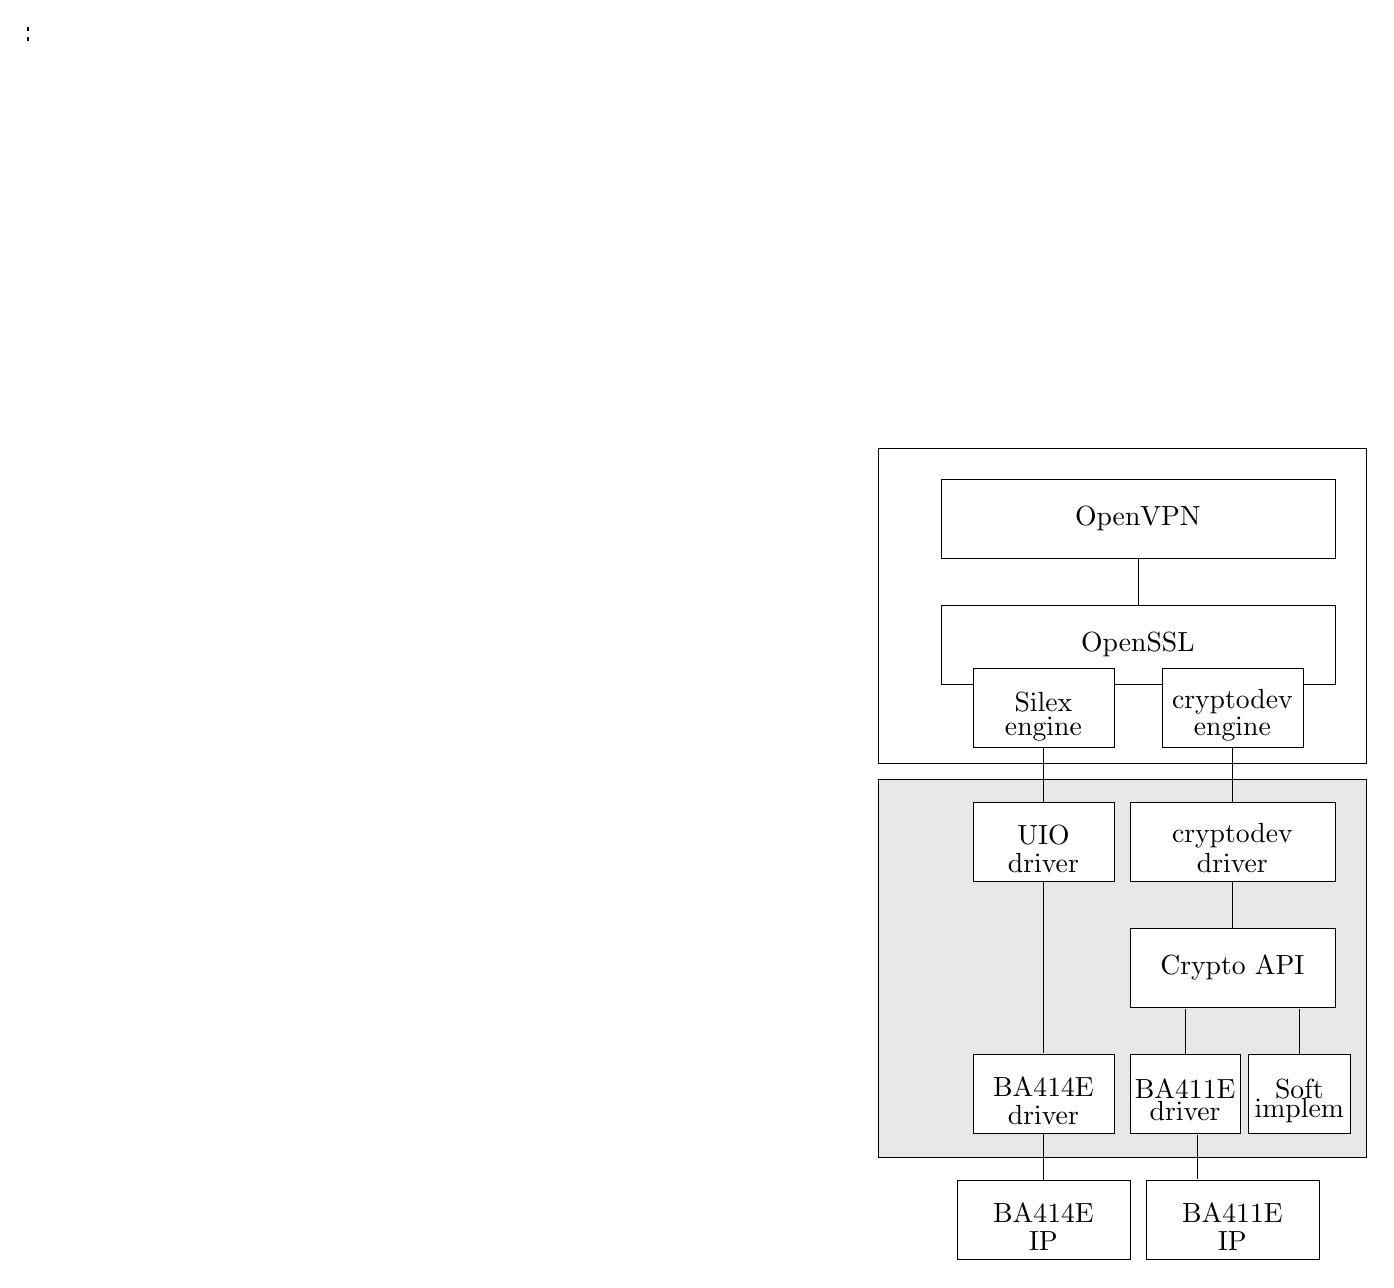
\begin{tikzpicture}
\pgftransformxscale{1.000000}
\pgftransformyscale{-1.000000}
\definecolor{dialinecolor}{rgb}{0.000000, 0.000000, 0.000000}
\pgfsetstrokecolor{dialinecolor}
\definecolor{dialinecolor}{rgb}{1.000000, 1.000000, 1.000000}
\pgfsetfillcolor{dialinecolor}
\pgfsetlinewidth{0.050000\du}
\pgfsetdash{}{0pt}
\pgfsetdash{}{0pt}
\pgfsetmiterjoin
\definecolor{dialinecolor}{rgb}{1.000000, 1.000000, 1.000000}
\pgfsetfillcolor{dialinecolor}
\fill (11.200000\du,5.600000\du)--(11.200000\du,9.600000\du)--(17.400000\du,9.600000\du)--(17.400000\du,5.600000\du)--cycle;
\definecolor{dialinecolor}{rgb}{0.000000, 0.000000, 0.000000}
\pgfsetstrokecolor{dialinecolor}
\draw (11.200000\du,5.600000\du)--(11.200000\du,9.600000\du)--(17.400000\du,9.600000\du)--(17.400000\du,5.600000\du)--cycle;
\pgfsetlinewidth{0.050000\du}
\pgfsetdash{}{0pt}
\pgfsetdash{}{0pt}
\pgfsetmiterjoin
\definecolor{dialinecolor}{rgb}{0.905882, 0.905882, 0.905882}
\pgfsetfillcolor{dialinecolor}
\fill (11.200000\du,9.800000\du)--(11.200000\du,14.600000\du)--(17.400000\du,14.600000\du)--(17.400000\du,9.800000\du)--cycle;
\definecolor{dialinecolor}{rgb}{0.000000, 0.000000, 0.000000}
\pgfsetstrokecolor{dialinecolor}
\draw (11.200000\du,9.800000\du)--(11.200000\du,14.600000\du)--(17.400000\du,14.600000\du)--(17.400000\du,9.800000\du)--cycle;
\pgfsetlinewidth{0.000000\du}
\pgfsetdash{}{0pt}
\pgfsetmiterjoin
\pgfsetroundcap
\definecolor{dialinecolor}{rgb}{0.000000, 0.000000, 0.000000}
\pgfsetfillcolor{dialinecolor}
\pgfpathmoveto{\pgfpoint{11.385372\du}{8.406740\du}}
\pgfpathlineto{\pgfpoint{11.392021\du}{8.357779\du}}
\pgfpathlineto{\pgfpoint{11.600318\du}{8.366119\du}}
\pgfpathcurveto{\pgfpoint{11.623347\du}{8.361767\du}}{\pgfpoint{11.642539\du}{8.358140\du}}{\pgfpoint{11.661731\du}{8.354513\du}}
\pgfpathcurveto{\pgfpoint{11.671795\du}{8.344661\du}}{\pgfpoint{11.678957\du}{8.319455\du}}{\pgfpoint{11.680831\du}{8.287297\du}}
\pgfpathcurveto{\pgfpoint{11.677204\du}{8.268106\du}}{\pgfpoint{11.669739\du}{8.249640\du}}{\pgfpoint{11.653872\du}{8.228786\du}}
\pgfpathcurveto{\pgfpoint{11.642569\du}{8.211045\du}}{\pgfpoint{11.625039\du}{8.202432\du}}{\pgfpoint{11.602009\du}{8.206784\du}}
\pgfpathlineto{\pgfpoint{11.393713\du}{8.198443\du}}
\pgfpathlineto{\pgfpoint{11.387910\du}{8.167737\du}}
\pgfpathlineto{\pgfpoint{11.596206\du}{8.176077\du}}
\pgfpathcurveto{\pgfpoint{11.638428\du}{8.168098\du}}{\pgfpoint{11.665085\du}{8.182938\du}}{\pgfpoint{11.681677\du}{8.207630\du}}
\pgfpathcurveto{\pgfpoint{11.705221\du}{8.227033\du}}{\pgfpoint{11.714137\du}{8.253176\du}}{\pgfpoint{11.711538\du}{8.281495\du}}
\pgfpathcurveto{\pgfpoint{11.708002\du}{8.325892\du}}{\pgfpoint{11.698451\du}{8.359500\du}}{\pgfpoint{11.682887\du}{8.382318\du}}
\pgfpathcurveto{\pgfpoint{11.665871\du}{8.397460\du}}{\pgfpoint{11.635890\du}{8.407101\du}}{\pgfpoint{11.593669\du}{8.415080\du}}
\pgfpathlineto{\pgfpoint{11.385372\du}{8.406740\du}}
\pgfusepath{fill}
\definecolor{dialinecolor}{rgb}{0.000000, 0.000000, 0.000000}
\pgfsetfillcolor{dialinecolor}
\pgfpathmoveto{\pgfpoint{11.483081\du}{7.935080\du}}
\pgfpathlineto{\pgfpoint{11.516689\du}{7.944630\du}}
\pgfpathcurveto{\pgfpoint{11.518865\du}{7.956145\du}}{\pgfpoint{11.521041\du}{7.967660\du}}{\pgfpoint{11.522492\du}{7.975337\du}}
\pgfpathcurveto{\pgfpoint{11.516991\du}{7.988303\du}}{\pgfpoint{11.508378\du}{8.005832\du}}{\pgfpoint{11.500490\du}{8.027200\du}}
\pgfpathcurveto{\pgfpoint{11.502666\du}{8.038714\du}}{\pgfpoint{11.512519\du}{8.048779\du}}{\pgfpoint{11.521646\du}{8.055005\du}}
\pgfpathcurveto{\pgfpoint{11.523822\du}{8.066520\du}}{\pgfpoint{11.532224\du}{8.068907\du}}{\pgfpoint{11.539901\du}{8.067456\du}}
\pgfpathcurveto{\pgfpoint{11.551416\du}{8.065280\du}}{\pgfpoint{11.562931\du}{8.063104\du}}{\pgfpoint{11.570607\du}{8.061653\du}}
\pgfpathcurveto{\pgfpoint{11.569156\du}{8.053977\du}}{\pgfpoint{11.573932\du}{8.037173\du}}{\pgfpoint{11.577256\du}{8.012692\du}}
\pgfpathlineto{\pgfpoint{11.574355\du}{7.997339\du}}
\pgfpathcurveto{\pgfpoint{11.584419\du}{7.987486\du}}{\pgfpoint{11.593758\du}{7.973795\du}}{\pgfpoint{11.599258\du}{7.960830\du}}
\pgfpathcurveto{\pgfpoint{11.609322\du}{7.950977\du}}{\pgfpoint{11.623225\du}{7.940399\du}}{\pgfpoint{11.642416\du}{7.936772\du}}
\pgfpathcurveto{\pgfpoint{11.667622\du}{7.943935\du}}{\pgfpoint{11.681313\du}{7.953273\du}}{\pgfpoint{11.694279\du}{7.958774\du}}
\pgfpathcurveto{\pgfpoint{11.704132\du}{7.968838\du}}{\pgfpoint{11.708484\du}{7.991868\du}}{\pgfpoint{11.705885\du}{8.020187\du}}
\pgfpathcurveto{\pgfpoint{11.710237\du}{8.043217\du}}{\pgfpoint{11.713139\du}{8.058570\du}}{\pgfpoint{11.714589\du}{8.066247\du}}
\pgfpathcurveto{\pgfpoint{11.716765\du}{8.077762\du}}{\pgfpoint{11.711990\du}{8.094566\du}}{\pgfpoint{11.707940\du}{8.115208\du}}
\pgfpathlineto{\pgfpoint{11.658979\du}{8.108559\du}}
\pgfpathcurveto{\pgfpoint{11.680558\du}{8.096530\du}}{\pgfpoint{11.686059\du}{8.083565\du}}{\pgfpoint{11.683883\du}{8.072050\du}}
\pgfpathcurveto{\pgfpoint{11.682432\du}{8.064373\du}}{\pgfpoint{11.679531\du}{8.049020\du}}{\pgfpoint{11.675178\du}{8.025990\du}}
\pgfpathcurveto{\pgfpoint{11.685243\du}{8.016137\du}}{\pgfpoint{11.686905\du}{8.003897\du}}{\pgfpoint{11.684729\du}{7.992382\du}}
\pgfpathcurveto{\pgfpoint{11.673425\du}{7.974641\du}}{\pgfpoint{11.659734\du}{7.965302\du}}{\pgfpoint{11.648219\du}{7.967478\du}}
\pgfpathcurveto{\pgfpoint{11.640543\du}{7.968929\du}}{\pgfpoint{11.634317\du}{7.978056\du}}{\pgfpoint{11.635767\du}{7.985733\du}}
\pgfpathcurveto{\pgfpoint{11.628091\du}{7.987184\du}}{\pgfpoint{11.618752\du}{8.000875\du}}{\pgfpoint{11.610864\du}{8.022243\du}}
\pgfpathlineto{\pgfpoint{11.598412\du}{8.040497\du}}
\pgfpathcurveto{\pgfpoint{11.604215\du}{8.071204\du}}{\pgfpoint{11.603278\du}{8.087282\du}}{\pgfpoint{11.591763\du}{8.089458\du}}
\pgfpathcurveto{\pgfpoint{11.572572\du}{8.093085\du}}{\pgfpoint{11.553380\du}{8.096712\du}}{\pgfpoint{11.530350\du}{8.101064\du}}
\pgfpathcurveto{\pgfpoint{11.522674\du}{8.102515\du}}{\pgfpoint{11.509708\du}{8.097015\du}}{\pgfpoint{11.493841\du}{8.076161\du}}
\pgfpathcurveto{\pgfpoint{11.482537\du}{8.058420\du}}{\pgfpoint{11.471234\du}{8.040679\du}}{\pgfpoint{11.466882\du}{8.017649\du}}
\pgfpathcurveto{\pgfpoint{11.476946\du}{8.007797\du}}{\pgfpoint{11.478608\du}{7.995556\du}}{\pgfpoint{11.476432\du}{7.984041\du}}
\pgfpathcurveto{\pgfpoint{11.472805\du}{7.964850\du}}{\pgfpoint{11.477580\du}{7.948046\du}}{\pgfpoint{11.483081\du}{7.935080\du}}
\pgfpathlineto{\pgfpoint{11.483081\du}{7.935080\du}}
\pgfusepath{fill}
\definecolor{dialinecolor}{rgb}{0.000000, 0.000000, 0.000000}
\pgfsetfillcolor{dialinecolor}
\pgfpathmoveto{\pgfpoint{11.586140\du}{7.681056\du}}
\pgfpathlineto{\pgfpoint{11.601493\du}{7.678154\du}}
\pgfpathlineto{\pgfpoint{11.602703\du}{7.852843\du}}
\pgfpathcurveto{\pgfpoint{11.633410\du}{7.847040\du}}{\pgfpoint{11.655714\du}{7.838850\du}}{\pgfpoint{11.661215\du}{7.825884\du}}
\pgfpathcurveto{\pgfpoint{11.671279\du}{7.816031\du}}{\pgfpoint{11.679892\du}{7.798502\du}}{\pgfpoint{11.683217\du}{7.774021\du}}
\pgfpathcurveto{\pgfpoint{11.681766\du}{7.766345\du}}{\pgfpoint{11.679590\du}{7.754830\du}}{\pgfpoint{11.677414\du}{7.743315\du}}
\pgfpathcurveto{\pgfpoint{11.681463\du}{7.722672\du}}{\pgfpoint{11.676386\du}{7.695804\du}}{\pgfpoint{11.662906\du}{7.666548\du}}
\pgfpathlineto{\pgfpoint{11.696514\du}{7.676099\du}}
\pgfpathcurveto{\pgfpoint{11.708543\du}{7.697678\du}}{\pgfpoint{11.712170\du}{7.716869\du}}{\pgfpoint{11.708120\du}{7.737512\du}}
\pgfpathcurveto{\pgfpoint{11.710296\du}{7.749027\du}}{\pgfpoint{11.712472\du}{7.760542\du}}{\pgfpoint{11.713923\du}{7.768218\du}}
\pgfpathcurveto{\pgfpoint{11.710387\du}{7.812616\du}}{\pgfpoint{11.700112\du}{7.842385\du}}{\pgfpoint{11.682371\du}{7.853689\du}}
\pgfpathcurveto{\pgfpoint{11.657679\du}{7.870281\du}}{\pgfpoint{11.623859\du}{7.880648\du}}{\pgfpoint{11.593153\du}{7.886451\du}}
\pgfpathcurveto{\pgfpoint{11.553319\du}{7.886028\du}}{\pgfpoint{11.523549\du}{7.875752\du}}{\pgfpoint{11.507682\du}{7.854899\du}}
\pgfpathcurveto{\pgfpoint{11.484864\du}{7.839334\du}}{\pgfpoint{11.475222\du}{7.809353\du}}{\pgfpoint{11.474920\du}{7.765681\du}}
\pgfpathcurveto{\pgfpoint{11.469842\du}{7.738812\du}}{\pgfpoint{11.484682\du}{7.712156\du}}{\pgfpoint{11.509374\du}{7.695563\du}}
\pgfpathcurveto{\pgfpoint{11.530953\du}{7.683534\du}}{\pgfpoint{11.557821\du}{7.678457\du}}{\pgfpoint{11.586140\du}{7.681056\du}}
\pgfpathlineto{\pgfpoint{11.586140\du}{7.681056\du}}
\pgfusepath{fill}
\definecolor{dialinecolor}{rgb}{1.000000, 1.000000, 1.000000}
\pgfsetfillcolor{dialinecolor}
\pgfpathmoveto{\pgfpoint{11.561237\du}{7.717565\du}}
\pgfpathcurveto{\pgfpoint{11.553560\du}{7.719016\du}}{\pgfpoint{11.543496\du}{7.728869\du}}{\pgfpoint{11.533432\du}{7.738721\du}}
\pgfpathcurveto{\pgfpoint{11.516416\du}{7.753863\du}}{\pgfpoint{11.507077\du}{7.767554\du}}{\pgfpoint{11.508528\du}{7.775231\du}}
\pgfpathcurveto{\pgfpoint{11.505204\du}{7.799711\du}}{\pgfpoint{11.508830\du}{7.818903\du}}{\pgfpoint{11.520134\du}{7.836644\du}}
\pgfpathcurveto{\pgfpoint{11.533825\du}{7.845983\du}}{\pgfpoint{11.549904\du}{7.846919\du}}{\pgfpoint{11.569095\du}{7.843293\du}}
\pgfusepath{fill}
\definecolor{dialinecolor}{rgb}{0.000000, 0.000000, 0.000000}
\pgfsetfillcolor{dialinecolor}
\pgfpathmoveto{\pgfpoint{11.520102\du}{7.478865\du}}
\pgfpathcurveto{\pgfpoint{11.522278\du}{7.490379\du}}{\pgfpoint{11.523004\du}{7.494218\du}}{\pgfpoint{11.523004\du}{7.494218\du}}
\pgfpathcurveto{\pgfpoint{11.515327\du}{7.495669\du}}{\pgfpoint{11.509101\du}{7.504796\du}}{\pgfpoint{11.510552\du}{7.512473\du}}
\pgfpathcurveto{\pgfpoint{11.507227\du}{7.536953\du}}{\pgfpoint{11.513967\du}{7.551581\du}}{\pgfpoint{11.534610\du}{7.555631\du}}
\pgfpathcurveto{\pgfpoint{11.548301\du}{7.564970\du}}{\pgfpoint{11.573507\du}{7.572132\du}}{\pgfpoint{11.601825\du}{7.574731\du}}
\pgfpathlineto{\pgfpoint{11.712200\du}{7.569774\du}}
\pgfpathlineto{\pgfpoint{11.705551\du}{7.618736\du}}
\pgfpathlineto{\pgfpoint{11.466548\du}{7.616198\du}}
\pgfpathlineto{\pgfpoint{11.473197\du}{7.567237\du}}
\pgfpathlineto{\pgfpoint{11.522158\du}{7.573885\du}}
\pgfpathcurveto{\pgfpoint{11.501515\du}{7.569836\du}}{\pgfpoint{11.487824\du}{7.560497\du}}{\pgfpoint{11.485648\du}{7.548982\du}}
\pgfpathcurveto{\pgfpoint{11.474345\du}{7.531241\du}}{\pgfpoint{11.470718\du}{7.512050\du}}{\pgfpoint{11.474042\du}{7.487569\du}}
\pgfpathcurveto{\pgfpoint{11.474042\du}{7.487569\du}}{\pgfpoint{11.473317\du}{7.483731\du}}{\pgfpoint{11.471141\du}{7.472216\du}}
\pgfpathlineto{\pgfpoint{11.520102\du}{7.478865\du}}
\pgfusepath{fill}
\definecolor{dialinecolor}{rgb}{0.000000, 0.000000, 0.000000}
\pgfsetstrokecolor{dialinecolor}
\pgfpathmoveto{\pgfpoint{11.385372\du}{8.406740\du}}
\pgfpathlineto{\pgfpoint{11.392021\du}{8.357779\du}}
\pgfpathlineto{\pgfpoint{11.600318\du}{8.366119\du}}
\pgfpathcurveto{\pgfpoint{11.623347\du}{8.361767\du}}{\pgfpoint{11.642539\du}{8.358140\du}}{\pgfpoint{11.661731\du}{8.354513\du}}
\pgfpathcurveto{\pgfpoint{11.671795\du}{8.344661\du}}{\pgfpoint{11.678957\du}{8.319455\du}}{\pgfpoint{11.680831\du}{8.287297\du}}
\pgfpathcurveto{\pgfpoint{11.677204\du}{8.268106\du}}{\pgfpoint{11.669739\du}{8.249640\du}}{\pgfpoint{11.653872\du}{8.228786\du}}
\pgfpathcurveto{\pgfpoint{11.642569\du}{8.211045\du}}{\pgfpoint{11.625039\du}{8.202432\du}}{\pgfpoint{11.602009\du}{8.206784\du}}
\pgfpathlineto{\pgfpoint{11.393713\du}{8.198443\du}}
\pgfpathlineto{\pgfpoint{11.387910\du}{8.167737\du}}
\pgfpathlineto{\pgfpoint{11.596206\du}{8.176077\du}}
\pgfpathcurveto{\pgfpoint{11.638428\du}{8.168098\du}}{\pgfpoint{11.665085\du}{8.182938\du}}{\pgfpoint{11.681677\du}{8.207630\du}}
\pgfpathcurveto{\pgfpoint{11.705221\du}{8.227033\du}}{\pgfpoint{11.714137\du}{8.253176\du}}{\pgfpoint{11.711538\du}{8.281495\du}}
\pgfpathcurveto{\pgfpoint{11.708002\du}{8.325892\du}}{\pgfpoint{11.698451\du}{8.359500\du}}{\pgfpoint{11.682887\du}{8.382318\du}}
\pgfpathcurveto{\pgfpoint{11.665871\du}{8.397460\du}}{\pgfpoint{11.635890\du}{8.407101\du}}{\pgfpoint{11.593669\du}{8.415080\du}}
\pgfpathlineto{\pgfpoint{11.385372\du}{8.406740\du}}
\pgfusepath{stroke}
\definecolor{dialinecolor}{rgb}{0.000000, 0.000000, 0.000000}
\pgfsetstrokecolor{dialinecolor}
\pgfpathmoveto{\pgfpoint{11.483081\du}{7.935080\du}}
\pgfpathlineto{\pgfpoint{11.516689\du}{7.944630\du}}
\pgfpathcurveto{\pgfpoint{11.518865\du}{7.956145\du}}{\pgfpoint{11.521041\du}{7.967660\du}}{\pgfpoint{11.522492\du}{7.975337\du}}
\pgfpathcurveto{\pgfpoint{11.516991\du}{7.988303\du}}{\pgfpoint{11.508378\du}{8.005832\du}}{\pgfpoint{11.500490\du}{8.027200\du}}
\pgfpathcurveto{\pgfpoint{11.502666\du}{8.038714\du}}{\pgfpoint{11.512519\du}{8.048779\du}}{\pgfpoint{11.521646\du}{8.055005\du}}
\pgfpathcurveto{\pgfpoint{11.523822\du}{8.066520\du}}{\pgfpoint{11.532224\du}{8.068907\du}}{\pgfpoint{11.539901\du}{8.067456\du}}
\pgfpathcurveto{\pgfpoint{11.551416\du}{8.065280\du}}{\pgfpoint{11.562931\du}{8.063104\du}}{\pgfpoint{11.570607\du}{8.061653\du}}
\pgfpathcurveto{\pgfpoint{11.569156\du}{8.053977\du}}{\pgfpoint{11.573932\du}{8.037173\du}}{\pgfpoint{11.577256\du}{8.012692\du}}
\pgfpathlineto{\pgfpoint{11.574355\du}{7.997339\du}}
\pgfpathcurveto{\pgfpoint{11.584419\du}{7.987486\du}}{\pgfpoint{11.593758\du}{7.973795\du}}{\pgfpoint{11.599258\du}{7.960830\du}}
\pgfpathcurveto{\pgfpoint{11.609322\du}{7.950977\du}}{\pgfpoint{11.623225\du}{7.940399\du}}{\pgfpoint{11.642416\du}{7.936772\du}}
\pgfpathcurveto{\pgfpoint{11.667622\du}{7.943935\du}}{\pgfpoint{11.681313\du}{7.953273\du}}{\pgfpoint{11.694279\du}{7.958774\du}}
\pgfpathcurveto{\pgfpoint{11.704132\du}{7.968838\du}}{\pgfpoint{11.708484\du}{7.991868\du}}{\pgfpoint{11.705885\du}{8.020187\du}}
\pgfpathcurveto{\pgfpoint{11.710237\du}{8.043217\du}}{\pgfpoint{11.713139\du}{8.058570\du}}{\pgfpoint{11.714589\du}{8.066247\du}}
\pgfpathcurveto{\pgfpoint{11.716765\du}{8.077762\du}}{\pgfpoint{11.711990\du}{8.094566\du}}{\pgfpoint{11.707940\du}{8.115208\du}}
\pgfpathlineto{\pgfpoint{11.658979\du}{8.108559\du}}
\pgfpathcurveto{\pgfpoint{11.680558\du}{8.096530\du}}{\pgfpoint{11.686059\du}{8.083565\du}}{\pgfpoint{11.683883\du}{8.072050\du}}
\pgfpathcurveto{\pgfpoint{11.682432\du}{8.064373\du}}{\pgfpoint{11.679531\du}{8.049020\du}}{\pgfpoint{11.675178\du}{8.025990\du}}
\pgfpathcurveto{\pgfpoint{11.685243\du}{8.016137\du}}{\pgfpoint{11.686905\du}{8.003897\du}}{\pgfpoint{11.684729\du}{7.992382\du}}
\pgfpathcurveto{\pgfpoint{11.673425\du}{7.974641\du}}{\pgfpoint{11.659734\du}{7.965302\du}}{\pgfpoint{11.648219\du}{7.967478\du}}
\pgfpathcurveto{\pgfpoint{11.640543\du}{7.968929\du}}{\pgfpoint{11.634317\du}{7.978056\du}}{\pgfpoint{11.635767\du}{7.985733\du}}
\pgfpathcurveto{\pgfpoint{11.628091\du}{7.987184\du}}{\pgfpoint{11.618752\du}{8.000875\du}}{\pgfpoint{11.610864\du}{8.022243\du}}
\pgfpathlineto{\pgfpoint{11.598412\du}{8.040497\du}}
\pgfpathcurveto{\pgfpoint{11.604215\du}{8.071204\du}}{\pgfpoint{11.603278\du}{8.087282\du}}{\pgfpoint{11.591763\du}{8.089458\du}}
\pgfpathcurveto{\pgfpoint{11.572572\du}{8.093085\du}}{\pgfpoint{11.553380\du}{8.096712\du}}{\pgfpoint{11.530350\du}{8.101064\du}}
\pgfpathcurveto{\pgfpoint{11.522674\du}{8.102515\du}}{\pgfpoint{11.509708\du}{8.097015\du}}{\pgfpoint{11.493841\du}{8.076161\du}}
\pgfpathcurveto{\pgfpoint{11.482537\du}{8.058420\du}}{\pgfpoint{11.471234\du}{8.040679\du}}{\pgfpoint{11.466882\du}{8.017649\du}}
\pgfpathcurveto{\pgfpoint{11.476946\du}{8.007797\du}}{\pgfpoint{11.478608\du}{7.995556\du}}{\pgfpoint{11.476432\du}{7.984041\du}}
\pgfpathcurveto{\pgfpoint{11.472805\du}{7.964850\du}}{\pgfpoint{11.477580\du}{7.948046\du}}{\pgfpoint{11.483081\du}{7.935080\du}}
\pgfpathlineto{\pgfpoint{11.483081\du}{7.935080\du}}
\pgfusepath{stroke}
\definecolor{dialinecolor}{rgb}{0.000000, 0.000000, 0.000000}
\pgfsetstrokecolor{dialinecolor}
\pgfpathmoveto{\pgfpoint{11.586140\du}{7.681056\du}}
\pgfpathlineto{\pgfpoint{11.601493\du}{7.678154\du}}
\pgfpathlineto{\pgfpoint{11.602703\du}{7.852843\du}}
\pgfpathcurveto{\pgfpoint{11.633410\du}{7.847040\du}}{\pgfpoint{11.655714\du}{7.838850\du}}{\pgfpoint{11.661215\du}{7.825884\du}}
\pgfpathcurveto{\pgfpoint{11.671279\du}{7.816031\du}}{\pgfpoint{11.679892\du}{7.798502\du}}{\pgfpoint{11.683217\du}{7.774021\du}}
\pgfpathcurveto{\pgfpoint{11.681766\du}{7.766345\du}}{\pgfpoint{11.679590\du}{7.754830\du}}{\pgfpoint{11.677414\du}{7.743315\du}}
\pgfpathcurveto{\pgfpoint{11.681463\du}{7.722672\du}}{\pgfpoint{11.676386\du}{7.695804\du}}{\pgfpoint{11.662906\du}{7.666548\du}}
\pgfpathlineto{\pgfpoint{11.696514\du}{7.676099\du}}
\pgfpathcurveto{\pgfpoint{11.708543\du}{7.697678\du}}{\pgfpoint{11.712170\du}{7.716869\du}}{\pgfpoint{11.708120\du}{7.737512\du}}
\pgfpathcurveto{\pgfpoint{11.710296\du}{7.749027\du}}{\pgfpoint{11.712472\du}{7.760542\du}}{\pgfpoint{11.713923\du}{7.768218\du}}
\pgfpathcurveto{\pgfpoint{11.710387\du}{7.812616\du}}{\pgfpoint{11.700112\du}{7.842385\du}}{\pgfpoint{11.682371\du}{7.853689\du}}
\pgfpathcurveto{\pgfpoint{11.657679\du}{7.870281\du}}{\pgfpoint{11.623859\du}{7.880648\du}}{\pgfpoint{11.593153\du}{7.886451\du}}
\pgfpathcurveto{\pgfpoint{11.553319\du}{7.886028\du}}{\pgfpoint{11.523549\du}{7.875752\du}}{\pgfpoint{11.507682\du}{7.854899\du}}
\pgfpathcurveto{\pgfpoint{11.484864\du}{7.839334\du}}{\pgfpoint{11.475222\du}{7.809353\du}}{\pgfpoint{11.474920\du}{7.765681\du}}
\pgfpathcurveto{\pgfpoint{11.469842\du}{7.738812\du}}{\pgfpoint{11.484682\du}{7.712156\du}}{\pgfpoint{11.509374\du}{7.695563\du}}
\pgfpathcurveto{\pgfpoint{11.530953\du}{7.683534\du}}{\pgfpoint{11.557821\du}{7.678457\du}}{\pgfpoint{11.586140\du}{7.681056\du}}
\pgfpathlineto{\pgfpoint{11.586140\du}{7.681056\du}}
\pgfusepath{stroke}
\definecolor{dialinecolor}{rgb}{0.000000, 0.000000, 0.000000}
\pgfsetstrokecolor{dialinecolor}
\pgfpathmoveto{\pgfpoint{11.561237\du}{7.717565\du}}
\pgfpathcurveto{\pgfpoint{11.553560\du}{7.719016\du}}{\pgfpoint{11.543496\du}{7.728869\du}}{\pgfpoint{11.533432\du}{7.738721\du}}
\pgfpathcurveto{\pgfpoint{11.516416\du}{7.753863\du}}{\pgfpoint{11.507077\du}{7.767554\du}}{\pgfpoint{11.508528\du}{7.775231\du}}
\pgfpathcurveto{\pgfpoint{11.505204\du}{7.799711\du}}{\pgfpoint{11.508830\du}{7.818903\du}}{\pgfpoint{11.520134\du}{7.836644\du}}
\pgfpathcurveto{\pgfpoint{11.533825\du}{7.845983\du}}{\pgfpoint{11.549904\du}{7.846919\du}}{\pgfpoint{11.569095\du}{7.843293\du}}
\pgfpathlineto{\pgfpoint{11.561237\du}{7.717565\du}}
\pgfusepath{stroke}
\definecolor{dialinecolor}{rgb}{0.000000, 0.000000, 0.000000}
\pgfsetstrokecolor{dialinecolor}
\pgfpathmoveto{\pgfpoint{11.520102\du}{7.478865\du}}
\pgfpathcurveto{\pgfpoint{11.522278\du}{7.490379\du}}{\pgfpoint{11.523004\du}{7.494218\du}}{\pgfpoint{11.523004\du}{7.494218\du}}
\pgfpathcurveto{\pgfpoint{11.515327\du}{7.495669\du}}{\pgfpoint{11.509101\du}{7.504796\du}}{\pgfpoint{11.510552\du}{7.512473\du}}
\pgfpathcurveto{\pgfpoint{11.507227\du}{7.536953\du}}{\pgfpoint{11.513967\du}{7.551581\du}}{\pgfpoint{11.534610\du}{7.555631\du}}
\pgfpathcurveto{\pgfpoint{11.548301\du}{7.564970\du}}{\pgfpoint{11.573507\du}{7.572132\du}}{\pgfpoint{11.601825\du}{7.574731\du}}
\pgfpathlineto{\pgfpoint{11.712200\du}{7.569774\du}}
\pgfpathlineto{\pgfpoint{11.705551\du}{7.618736\du}}
\pgfpathlineto{\pgfpoint{11.466548\du}{7.616198\du}}
\pgfpathlineto{\pgfpoint{11.473197\du}{7.567237\du}}
\pgfpathlineto{\pgfpoint{11.522158\du}{7.573885\du}}
\pgfpathcurveto{\pgfpoint{11.501515\du}{7.569836\du}}{\pgfpoint{11.487824\du}{7.560497\du}}{\pgfpoint{11.485648\du}{7.548982\du}}
\pgfpathcurveto{\pgfpoint{11.474345\du}{7.531241\du}}{\pgfpoint{11.470718\du}{7.512050\du}}{\pgfpoint{11.474042\du}{7.487569\du}}
\pgfpathcurveto{\pgfpoint{11.474042\du}{7.487569\du}}{\pgfpoint{11.473317\du}{7.483731\du}}{\pgfpoint{11.471141\du}{7.472216\du}}
\pgfpathlineto{\pgfpoint{11.520102\du}{7.478865\du}}
\pgfusepath{stroke}
\pgfsetlinewidth{0.000000\du}
\pgfsetdash{}{0pt}
\pgfsetmiterjoin
\pgfsetroundcap
\definecolor{dialinecolor}{rgb}{0.000000, 0.000000, 0.000000}
\pgfsetfillcolor{dialinecolor}
\pgfpathmoveto{\pgfpoint{11.400725\du}{12.203838\du}}
\pgfpathlineto{\pgfpoint{11.407374\du}{12.154877\du}}
\pgfpathlineto{\pgfpoint{11.551356\du}{12.159470\du}}
\pgfpathlineto{\pgfpoint{11.411968\du}{12.010895\du}}
\pgfpathlineto{\pgfpoint{11.403263\du}{11.964835\du}}
\pgfpathlineto{\pgfpoint{11.558005\du}{12.110509\du}}
\pgfpathlineto{\pgfpoint{11.719032\du}{11.952866\du}}
\pgfpathlineto{\pgfpoint{11.727737\du}{11.998925\du}}
\pgfpathlineto{\pgfpoint{11.582063\du}{12.153667\du}}
\pgfpathlineto{\pgfpoint{11.726045\du}{12.158261\du}}
\pgfpathlineto{\pgfpoint{11.719396\du}{12.207222\du}}
\pgfpathlineto{\pgfpoint{11.400725\du}{12.203838\du}}
\pgfusepath{fill}
\definecolor{dialinecolor}{rgb}{0.000000, 0.000000, 0.000000}
\pgfsetfillcolor{dialinecolor}
\pgfpathmoveto{\pgfpoint{11.601132\du}{11.728672\du}}
\pgfpathlineto{\pgfpoint{11.616485\du}{11.725771\du}}
\pgfpathlineto{\pgfpoint{11.617695\du}{11.900459\du}}
\pgfpathcurveto{\pgfpoint{11.648401\du}{11.894657\du}}{\pgfpoint{11.670706\du}{11.886466\du}}{\pgfpoint{11.676206\du}{11.873500\du}}
\pgfpathcurveto{\pgfpoint{11.686270\du}{11.863648\du}}{\pgfpoint{11.694884\du}{11.846118\du}}{\pgfpoint{11.698208\du}{11.821638\du}}
\pgfpathcurveto{\pgfpoint{11.696758\du}{11.813961\du}}{\pgfpoint{11.694581\du}{11.802446\du}}{\pgfpoint{11.692405\du}{11.790931\du}}
\pgfpathcurveto{\pgfpoint{11.696455\du}{11.770289\du}}{\pgfpoint{11.691378\du}{11.743421\du}}{\pgfpoint{11.677898\du}{11.714165\du}}
\pgfpathlineto{\pgfpoint{11.711506\du}{11.723715\du}}
\pgfpathcurveto{\pgfpoint{11.723535\du}{11.745294\du}}{\pgfpoint{11.727162\du}{11.764486\du}}{\pgfpoint{11.723112\du}{11.785128\du}}
\pgfpathcurveto{\pgfpoint{11.725288\du}{11.796643\du}}{\pgfpoint{11.727464\du}{11.808158\du}}{\pgfpoint{11.728915\du}{11.815835\du}}
\pgfpathcurveto{\pgfpoint{11.725379\du}{11.860232\du}}{\pgfpoint{11.715103\du}{11.890002\du}}{\pgfpoint{11.697362\du}{11.901305\du}}
\pgfpathcurveto{\pgfpoint{11.672670\du}{11.917898\du}}{\pgfpoint{11.638851\du}{11.928265\du}}{\pgfpoint{11.608144\du}{11.934067\du}}
\pgfpathcurveto{\pgfpoint{11.568310\du}{11.933644\du}}{\pgfpoint{11.538541\du}{11.923369\du}}{\pgfpoint{11.522674\du}{11.902515\du}}
\pgfpathcurveto{\pgfpoint{11.499855\du}{11.886950\du}}{\pgfpoint{11.490214\du}{11.856969\du}}{\pgfpoint{11.489912\du}{11.813297\du}}
\pgfpathcurveto{\pgfpoint{11.484834\du}{11.786429\du}}{\pgfpoint{11.499673\du}{11.759772\du}}{\pgfpoint{11.524366\du}{11.743180\du}}
\pgfpathcurveto{\pgfpoint{11.545945\du}{11.731151\du}}{\pgfpoint{11.572813\du}{11.726073\du}}{\pgfpoint{11.601132\du}{11.728672\du}}
\pgfpathlineto{\pgfpoint{11.601132\du}{11.728672\du}}
\pgfusepath{fill}
\definecolor{dialinecolor}{rgb}{1.000000, 1.000000, 1.000000}
\pgfsetfillcolor{dialinecolor}
\pgfpathmoveto{\pgfpoint{11.576228\du}{11.765182\du}}
\pgfpathcurveto{\pgfpoint{11.568552\du}{11.766632\du}}{\pgfpoint{11.558487\du}{11.776485\du}}{\pgfpoint{11.548423\du}{11.786338\du}}
\pgfpathcurveto{\pgfpoint{11.531408\du}{11.801480\du}}{\pgfpoint{11.522069\du}{11.815171\du}}{\pgfpoint{11.523520\du}{11.822847\du}}
\pgfpathcurveto{\pgfpoint{11.520195\du}{11.847328\du}}{\pgfpoint{11.523822\du}{11.866520\du}}{\pgfpoint{11.535125\du}{11.884260\du}}
\pgfpathcurveto{\pgfpoint{11.548817\du}{11.893599\du}}{\pgfpoint{11.564895\du}{11.894536\du}}{\pgfpoint{11.584087\du}{11.890909\du}}
\pgfusepath{fill}
\definecolor{dialinecolor}{rgb}{0.000000, 0.000000, 0.000000}
\pgfsetfillcolor{dialinecolor}
\pgfpathmoveto{\pgfpoint{11.535819\du}{11.530319\du}}
\pgfpathcurveto{\pgfpoint{11.537995\du}{11.541834\du}}{\pgfpoint{11.538721\du}{11.545673\du}}{\pgfpoint{11.538721\du}{11.545673\du}}
\pgfpathcurveto{\pgfpoint{11.531044\du}{11.547123\du}}{\pgfpoint{11.524818\du}{11.556251\du}}{\pgfpoint{11.526269\du}{11.563927\du}}
\pgfpathcurveto{\pgfpoint{11.522944\du}{11.588408\du}}{\pgfpoint{11.529684\du}{11.603036\du}}{\pgfpoint{11.550326\du}{11.607086\du}}
\pgfpathcurveto{\pgfpoint{11.564018\du}{11.616424\du}}{\pgfpoint{11.589223\du}{11.623587\du}}{\pgfpoint{11.617542\du}{11.626186\du}}
\pgfpathlineto{\pgfpoint{11.727917\du}{11.621229\du}}
\pgfpathlineto{\pgfpoint{11.721268\du}{11.670190\du}}
\pgfpathlineto{\pgfpoint{11.482265\du}{11.667653\du}}
\pgfpathlineto{\pgfpoint{11.488914\du}{11.618691\du}}
\pgfpathlineto{\pgfpoint{11.537875\du}{11.625340\du}}
\pgfpathcurveto{\pgfpoint{11.517232\du}{11.621291\du}}{\pgfpoint{11.503541\du}{11.611952\du}}{\pgfpoint{11.501365\du}{11.600437\du}}
\pgfpathcurveto{\pgfpoint{11.490062\du}{11.582696\du}}{\pgfpoint{11.486435\du}{11.563504\du}}{\pgfpoint{11.489759\du}{11.539024\du}}
\pgfpathcurveto{\pgfpoint{11.489759\du}{11.539024\du}}{\pgfpoint{11.489034\du}{11.535185\du}}{\pgfpoint{11.486858\du}{11.523671\du}}
\pgfpathlineto{\pgfpoint{11.535819\du}{11.530319\du}}
\pgfusepath{fill}
\definecolor{dialinecolor}{rgb}{0.000000, 0.000000, 0.000000}
\pgfsetfillcolor{dialinecolor}
\pgfpathmoveto{\pgfpoint{11.584417\du}{11.282612\du}}
\pgfpathlineto{\pgfpoint{11.728399\du}{11.287205\du}}
\pgfpathlineto{\pgfpoint{11.721750\du}{11.336166\du}}
\pgfpathlineto{\pgfpoint{11.577768\du}{11.331573\du}}
\pgfpathcurveto{\pgfpoint{11.558576\du}{11.335200\du}}{\pgfpoint{11.544674\du}{11.345778\du}}{\pgfpoint{11.534610\du}{11.355631\du}}
\pgfpathcurveto{\pgfpoint{11.526933\du}{11.357082\du}}{\pgfpoint{11.521432\du}{11.370047\du}}{\pgfpoint{11.525059\du}{11.389239\du}}
\pgfpathcurveto{\pgfpoint{11.521735\du}{11.413719\du}}{\pgfpoint{11.528475\du}{11.428347\du}}{\pgfpoint{11.549117\du}{11.432397\du}}
\pgfpathcurveto{\pgfpoint{11.562808\du}{11.441736\du}}{\pgfpoint{11.578886\du}{11.442673\du}}{\pgfpoint{11.598078\du}{11.439046\du}}
\pgfpathlineto{\pgfpoint{11.726707\du}{11.446541\du}}
\pgfpathlineto{\pgfpoint{11.720058\du}{11.495502\du}}
\pgfpathlineto{\pgfpoint{11.481055\du}{11.492964\du}}
\pgfpathlineto{\pgfpoint{11.487704\du}{11.444003\du}}
\pgfpathlineto{\pgfpoint{11.536665\du}{11.450652\du}}
\pgfpathcurveto{\pgfpoint{11.513847\du}{11.435087\du}}{\pgfpoint{11.499430\du}{11.421910\du}}{\pgfpoint{11.497254\du}{11.410395\du}}
\pgfpathcurveto{\pgfpoint{11.488127\du}{11.404169\du}}{\pgfpoint{11.485225\du}{11.388816\du}}{\pgfpoint{11.488550\du}{11.364335\du}}
\pgfpathcurveto{\pgfpoint{11.484923\du}{11.345144\du}}{\pgfpoint{11.493536\du}{11.327614\du}}{\pgfpoint{11.510552\du}{11.312473\du}}
\pgfpathcurveto{\pgfpoint{11.532131\du}{11.300444\du}}{\pgfpoint{11.557548\du}{11.287690\du}}{\pgfpoint{11.584417\du}{11.282612\du}}
\pgfpathlineto{\pgfpoint{11.584417\du}{11.282612\du}}
\pgfusepath{fill}
\definecolor{dialinecolor}{rgb}{0.000000, 0.000000, 0.000000}
\pgfsetfillcolor{dialinecolor}
\pgfpathmoveto{\pgfpoint{11.603244\du}{11.024629\du}}
\pgfpathlineto{\pgfpoint{11.618598\du}{11.021727\du}}
\pgfpathlineto{\pgfpoint{11.619807\du}{11.196416\du}}
\pgfpathcurveto{\pgfpoint{11.650514\du}{11.190613\du}}{\pgfpoint{11.672818\du}{11.182423\du}}{\pgfpoint{11.678319\du}{11.169457\du}}
\pgfpathcurveto{\pgfpoint{11.688383\du}{11.159604\du}}{\pgfpoint{11.696997\du}{11.142075\du}}{\pgfpoint{11.700321\du}{11.117594\du}}
\pgfpathcurveto{\pgfpoint{11.698870\du}{11.109918\du}}{\pgfpoint{11.696694\du}{11.098403\du}}{\pgfpoint{11.694518\du}{11.086888\du}}
\pgfpathcurveto{\pgfpoint{11.698568\du}{11.066245\du}}{\pgfpoint{11.693490\du}{11.039377\du}}{\pgfpoint{11.680011\du}{11.010121\du}}
\pgfpathlineto{\pgfpoint{11.713619\du}{11.019672\du}}
\pgfpathcurveto{\pgfpoint{11.725647\du}{11.041251\du}}{\pgfpoint{11.729274\du}{11.060442\du}}{\pgfpoint{11.725224\du}{11.081085\du}}
\pgfpathcurveto{\pgfpoint{11.727401\du}{11.092600\du}}{\pgfpoint{11.729577\du}{11.104115\du}}{\pgfpoint{11.731027\du}{11.111791\du}}
\pgfpathcurveto{\pgfpoint{11.727492\du}{11.156189\du}}{\pgfpoint{11.717216\du}{11.185958\du}}{\pgfpoint{11.699475\du}{11.197262\du}}
\pgfpathcurveto{\pgfpoint{11.674783\du}{11.213854\du}}{\pgfpoint{11.640964\du}{11.224221\du}}{\pgfpoint{11.610257\du}{11.230024\du}}
\pgfpathcurveto{\pgfpoint{11.570423\du}{11.229601\du}}{\pgfpoint{11.540654\du}{11.219325\du}}{\pgfpoint{11.524786\du}{11.198472\du}}
\pgfpathcurveto{\pgfpoint{11.501968\du}{11.182907\du}}{\pgfpoint{11.492327\du}{11.152926\du}}{\pgfpoint{11.492024\du}{11.109253\du}}
\pgfpathcurveto{\pgfpoint{11.486947\du}{11.082385\du}}{\pgfpoint{11.501786\du}{11.055729\du}}{\pgfpoint{11.526478\du}{11.039136\du}}
\pgfpathcurveto{\pgfpoint{11.548057\du}{11.027107\du}}{\pgfpoint{11.574926\du}{11.022030\du}}{\pgfpoint{11.603244\du}{11.024629\du}}
\pgfpathlineto{\pgfpoint{11.603244\du}{11.024629\du}}
\pgfusepath{fill}
\definecolor{dialinecolor}{rgb}{1.000000, 1.000000, 1.000000}
\pgfsetfillcolor{dialinecolor}
\pgfpathmoveto{\pgfpoint{11.578341\du}{11.061138\du}}
\pgfpathcurveto{\pgfpoint{11.570664\du}{11.062589\du}}{\pgfpoint{11.560600\du}{11.072442\du}}{\pgfpoint{11.550536\du}{11.082294\du}}
\pgfpathcurveto{\pgfpoint{11.533520\du}{11.097436\du}}{\pgfpoint{11.524182\du}{11.111127\du}}{\pgfpoint{11.525632\du}{11.118804\du}}
\pgfpathcurveto{\pgfpoint{11.522308\du}{11.143284\du}}{\pgfpoint{11.525935\du}{11.162476\du}}{\pgfpoint{11.537238\du}{11.180217\du}}
\pgfpathcurveto{\pgfpoint{11.550929\du}{11.189556\du}}{\pgfpoint{11.567008\du}{11.190492\du}}{\pgfpoint{11.586199\du}{11.186866\du}}
\pgfusepath{fill}
\definecolor{dialinecolor}{rgb}{0.000000, 0.000000, 0.000000}
\pgfsetfillcolor{dialinecolor}
\pgfpathmoveto{\pgfpoint{11.400871\du}{10.963489\du}}
\pgfpathlineto{\pgfpoint{11.407520\du}{10.914527\du}}
\pgfpathlineto{\pgfpoint{11.726191\du}{10.917911\du}}
\pgfpathlineto{\pgfpoint{11.719542\du}{10.966872\du}}
\pgfpathlineto{\pgfpoint{11.400871\du}{10.963489\du}}
\pgfusepath{fill}
\definecolor{dialinecolor}{rgb}{0.000000, 0.000000, 0.000000}
\pgfsetstrokecolor{dialinecolor}
\pgfpathmoveto{\pgfpoint{11.400725\du}{12.203838\du}}
\pgfpathlineto{\pgfpoint{11.407374\du}{12.154877\du}}
\pgfpathlineto{\pgfpoint{11.551356\du}{12.159470\du}}
\pgfpathlineto{\pgfpoint{11.411968\du}{12.010895\du}}
\pgfpathlineto{\pgfpoint{11.403263\du}{11.964835\du}}
\pgfpathlineto{\pgfpoint{11.558005\du}{12.110509\du}}
\pgfpathlineto{\pgfpoint{11.719032\du}{11.952866\du}}
\pgfpathlineto{\pgfpoint{11.727737\du}{11.998925\du}}
\pgfpathlineto{\pgfpoint{11.582063\du}{12.153667\du}}
\pgfpathlineto{\pgfpoint{11.726045\du}{12.158261\du}}
\pgfpathlineto{\pgfpoint{11.719396\du}{12.207222\du}}
\pgfpathlineto{\pgfpoint{11.400725\du}{12.203838\du}}
\pgfusepath{stroke}
\definecolor{dialinecolor}{rgb}{0.000000, 0.000000, 0.000000}
\pgfsetstrokecolor{dialinecolor}
\pgfpathmoveto{\pgfpoint{11.601132\du}{11.728672\du}}
\pgfpathlineto{\pgfpoint{11.616485\du}{11.725771\du}}
\pgfpathlineto{\pgfpoint{11.617695\du}{11.900459\du}}
\pgfpathcurveto{\pgfpoint{11.648401\du}{11.894657\du}}{\pgfpoint{11.670706\du}{11.886466\du}}{\pgfpoint{11.676206\du}{11.873500\du}}
\pgfpathcurveto{\pgfpoint{11.686270\du}{11.863648\du}}{\pgfpoint{11.694884\du}{11.846118\du}}{\pgfpoint{11.698208\du}{11.821638\du}}
\pgfpathcurveto{\pgfpoint{11.696758\du}{11.813961\du}}{\pgfpoint{11.694581\du}{11.802446\du}}{\pgfpoint{11.692405\du}{11.790931\du}}
\pgfpathcurveto{\pgfpoint{11.696455\du}{11.770289\du}}{\pgfpoint{11.691378\du}{11.743421\du}}{\pgfpoint{11.677898\du}{11.714165\du}}
\pgfpathlineto{\pgfpoint{11.711506\du}{11.723715\du}}
\pgfpathcurveto{\pgfpoint{11.723535\du}{11.745294\du}}{\pgfpoint{11.727162\du}{11.764486\du}}{\pgfpoint{11.723112\du}{11.785128\du}}
\pgfpathcurveto{\pgfpoint{11.725288\du}{11.796643\du}}{\pgfpoint{11.727464\du}{11.808158\du}}{\pgfpoint{11.728915\du}{11.815835\du}}
\pgfpathcurveto{\pgfpoint{11.725379\du}{11.860232\du}}{\pgfpoint{11.715103\du}{11.890002\du}}{\pgfpoint{11.697362\du}{11.901305\du}}
\pgfpathcurveto{\pgfpoint{11.672670\du}{11.917898\du}}{\pgfpoint{11.638851\du}{11.928265\du}}{\pgfpoint{11.608144\du}{11.934067\du}}
\pgfpathcurveto{\pgfpoint{11.568310\du}{11.933644\du}}{\pgfpoint{11.538541\du}{11.923369\du}}{\pgfpoint{11.522674\du}{11.902515\du}}
\pgfpathcurveto{\pgfpoint{11.499855\du}{11.886950\du}}{\pgfpoint{11.490214\du}{11.856969\du}}{\pgfpoint{11.489912\du}{11.813297\du}}
\pgfpathcurveto{\pgfpoint{11.484834\du}{11.786429\du}}{\pgfpoint{11.499673\du}{11.759772\du}}{\pgfpoint{11.524366\du}{11.743180\du}}
\pgfpathcurveto{\pgfpoint{11.545945\du}{11.731151\du}}{\pgfpoint{11.572813\du}{11.726073\du}}{\pgfpoint{11.601132\du}{11.728672\du}}
\pgfpathlineto{\pgfpoint{11.601132\du}{11.728672\du}}
\pgfusepath{stroke}
\definecolor{dialinecolor}{rgb}{0.000000, 0.000000, 0.000000}
\pgfsetstrokecolor{dialinecolor}
\pgfpathmoveto{\pgfpoint{11.576228\du}{11.765182\du}}
\pgfpathcurveto{\pgfpoint{11.568552\du}{11.766632\du}}{\pgfpoint{11.558487\du}{11.776485\du}}{\pgfpoint{11.548423\du}{11.786338\du}}
\pgfpathcurveto{\pgfpoint{11.531408\du}{11.801480\du}}{\pgfpoint{11.522069\du}{11.815171\du}}{\pgfpoint{11.523520\du}{11.822847\du}}
\pgfpathcurveto{\pgfpoint{11.520195\du}{11.847328\du}}{\pgfpoint{11.523822\du}{11.866520\du}}{\pgfpoint{11.535125\du}{11.884260\du}}
\pgfpathcurveto{\pgfpoint{11.548817\du}{11.893599\du}}{\pgfpoint{11.564895\du}{11.894536\du}}{\pgfpoint{11.584087\du}{11.890909\du}}
\pgfpathlineto{\pgfpoint{11.576228\du}{11.765182\du}}
\pgfusepath{stroke}
\definecolor{dialinecolor}{rgb}{0.000000, 0.000000, 0.000000}
\pgfsetstrokecolor{dialinecolor}
\pgfpathmoveto{\pgfpoint{11.535819\du}{11.530319\du}}
\pgfpathcurveto{\pgfpoint{11.537995\du}{11.541834\du}}{\pgfpoint{11.538721\du}{11.545673\du}}{\pgfpoint{11.538721\du}{11.545673\du}}
\pgfpathcurveto{\pgfpoint{11.531044\du}{11.547123\du}}{\pgfpoint{11.524818\du}{11.556251\du}}{\pgfpoint{11.526269\du}{11.563927\du}}
\pgfpathcurveto{\pgfpoint{11.522944\du}{11.588408\du}}{\pgfpoint{11.529684\du}{11.603036\du}}{\pgfpoint{11.550326\du}{11.607086\du}}
\pgfpathcurveto{\pgfpoint{11.564018\du}{11.616424\du}}{\pgfpoint{11.589223\du}{11.623587\du}}{\pgfpoint{11.617542\du}{11.626186\du}}
\pgfpathlineto{\pgfpoint{11.727917\du}{11.621229\du}}
\pgfpathlineto{\pgfpoint{11.721268\du}{11.670190\du}}
\pgfpathlineto{\pgfpoint{11.482265\du}{11.667653\du}}
\pgfpathlineto{\pgfpoint{11.488914\du}{11.618691\du}}
\pgfpathlineto{\pgfpoint{11.537875\du}{11.625340\du}}
\pgfpathcurveto{\pgfpoint{11.517232\du}{11.621291\du}}{\pgfpoint{11.503541\du}{11.611952\du}}{\pgfpoint{11.501365\du}{11.600437\du}}
\pgfpathcurveto{\pgfpoint{11.490062\du}{11.582696\du}}{\pgfpoint{11.486435\du}{11.563504\du}}{\pgfpoint{11.489759\du}{11.539024\du}}
\pgfpathcurveto{\pgfpoint{11.489759\du}{11.539024\du}}{\pgfpoint{11.489034\du}{11.535185\du}}{\pgfpoint{11.486858\du}{11.523671\du}}
\pgfpathlineto{\pgfpoint{11.535819\du}{11.530319\du}}
\pgfusepath{stroke}
\definecolor{dialinecolor}{rgb}{0.000000, 0.000000, 0.000000}
\pgfsetstrokecolor{dialinecolor}
\pgfpathmoveto{\pgfpoint{11.584417\du}{11.282612\du}}
\pgfpathlineto{\pgfpoint{11.728399\du}{11.287205\du}}
\pgfpathlineto{\pgfpoint{11.721750\du}{11.336166\du}}
\pgfpathlineto{\pgfpoint{11.577768\du}{11.331573\du}}
\pgfpathcurveto{\pgfpoint{11.558576\du}{11.335200\du}}{\pgfpoint{11.544674\du}{11.345778\du}}{\pgfpoint{11.534610\du}{11.355631\du}}
\pgfpathcurveto{\pgfpoint{11.526933\du}{11.357082\du}}{\pgfpoint{11.521432\du}{11.370047\du}}{\pgfpoint{11.525059\du}{11.389239\du}}
\pgfpathcurveto{\pgfpoint{11.521735\du}{11.413719\du}}{\pgfpoint{11.528475\du}{11.428347\du}}{\pgfpoint{11.549117\du}{11.432397\du}}
\pgfpathcurveto{\pgfpoint{11.562808\du}{11.441736\du}}{\pgfpoint{11.578886\du}{11.442673\du}}{\pgfpoint{11.598078\du}{11.439046\du}}
\pgfpathlineto{\pgfpoint{11.726707\du}{11.446541\du}}
\pgfpathlineto{\pgfpoint{11.720058\du}{11.495502\du}}
\pgfpathlineto{\pgfpoint{11.481055\du}{11.492964\du}}
\pgfpathlineto{\pgfpoint{11.487704\du}{11.444003\du}}
\pgfpathlineto{\pgfpoint{11.536665\du}{11.450652\du}}
\pgfpathcurveto{\pgfpoint{11.513847\du}{11.435087\du}}{\pgfpoint{11.499430\du}{11.421910\du}}{\pgfpoint{11.497254\du}{11.410395\du}}
\pgfpathcurveto{\pgfpoint{11.488127\du}{11.404169\du}}{\pgfpoint{11.485225\du}{11.388816\du}}{\pgfpoint{11.488550\du}{11.364335\du}}
\pgfpathcurveto{\pgfpoint{11.484923\du}{11.345144\du}}{\pgfpoint{11.493536\du}{11.327614\du}}{\pgfpoint{11.510552\du}{11.312473\du}}
\pgfpathcurveto{\pgfpoint{11.532131\du}{11.300444\du}}{\pgfpoint{11.557548\du}{11.287690\du}}{\pgfpoint{11.584417\du}{11.282612\du}}
\pgfpathlineto{\pgfpoint{11.584417\du}{11.282612\du}}
\pgfusepath{stroke}
\definecolor{dialinecolor}{rgb}{0.000000, 0.000000, 0.000000}
\pgfsetstrokecolor{dialinecolor}
\pgfpathmoveto{\pgfpoint{11.603244\du}{11.024629\du}}
\pgfpathlineto{\pgfpoint{11.618598\du}{11.021727\du}}
\pgfpathlineto{\pgfpoint{11.619807\du}{11.196416\du}}
\pgfpathcurveto{\pgfpoint{11.650514\du}{11.190613\du}}{\pgfpoint{11.672818\du}{11.182423\du}}{\pgfpoint{11.678319\du}{11.169457\du}}
\pgfpathcurveto{\pgfpoint{11.688383\du}{11.159604\du}}{\pgfpoint{11.696997\du}{11.142075\du}}{\pgfpoint{11.700321\du}{11.117594\du}}
\pgfpathcurveto{\pgfpoint{11.698870\du}{11.109918\du}}{\pgfpoint{11.696694\du}{11.098403\du}}{\pgfpoint{11.694518\du}{11.086888\du}}
\pgfpathcurveto{\pgfpoint{11.698568\du}{11.066245\du}}{\pgfpoint{11.693490\du}{11.039377\du}}{\pgfpoint{11.680011\du}{11.010121\du}}
\pgfpathlineto{\pgfpoint{11.713619\du}{11.019672\du}}
\pgfpathcurveto{\pgfpoint{11.725647\du}{11.041251\du}}{\pgfpoint{11.729274\du}{11.060442\du}}{\pgfpoint{11.725224\du}{11.081085\du}}
\pgfpathcurveto{\pgfpoint{11.727401\du}{11.092600\du}}{\pgfpoint{11.729577\du}{11.104115\du}}{\pgfpoint{11.731027\du}{11.111791\du}}
\pgfpathcurveto{\pgfpoint{11.727492\du}{11.156189\du}}{\pgfpoint{11.717216\du}{11.185958\du}}{\pgfpoint{11.699475\du}{11.197262\du}}
\pgfpathcurveto{\pgfpoint{11.674783\du}{11.213854\du}}{\pgfpoint{11.640964\du}{11.224221\du}}{\pgfpoint{11.610257\du}{11.230024\du}}
\pgfpathcurveto{\pgfpoint{11.570423\du}{11.229601\du}}{\pgfpoint{11.540654\du}{11.219325\du}}{\pgfpoint{11.524786\du}{11.198472\du}}
\pgfpathcurveto{\pgfpoint{11.501968\du}{11.182907\du}}{\pgfpoint{11.492327\du}{11.152926\du}}{\pgfpoint{11.492024\du}{11.109253\du}}
\pgfpathcurveto{\pgfpoint{11.486947\du}{11.082385\du}}{\pgfpoint{11.501786\du}{11.055729\du}}{\pgfpoint{11.526478\du}{11.039136\du}}
\pgfpathcurveto{\pgfpoint{11.548057\du}{11.027107\du}}{\pgfpoint{11.574926\du}{11.022030\du}}{\pgfpoint{11.603244\du}{11.024629\du}}
\pgfpathlineto{\pgfpoint{11.603244\du}{11.024629\du}}
\pgfusepath{stroke}
\definecolor{dialinecolor}{rgb}{0.000000, 0.000000, 0.000000}
\pgfsetstrokecolor{dialinecolor}
\pgfpathmoveto{\pgfpoint{11.578341\du}{11.061138\du}}
\pgfpathcurveto{\pgfpoint{11.570664\du}{11.062589\du}}{\pgfpoint{11.560600\du}{11.072442\du}}{\pgfpoint{11.550536\du}{11.082294\du}}
\pgfpathcurveto{\pgfpoint{11.533520\du}{11.097436\du}}{\pgfpoint{11.524182\du}{11.111127\du}}{\pgfpoint{11.525632\du}{11.118804\du}}
\pgfpathcurveto{\pgfpoint{11.522308\du}{11.143284\du}}{\pgfpoint{11.525935\du}{11.162476\du}}{\pgfpoint{11.537238\du}{11.180217\du}}
\pgfpathcurveto{\pgfpoint{11.550929\du}{11.189556\du}}{\pgfpoint{11.567008\du}{11.190492\du}}{\pgfpoint{11.586199\du}{11.186866\du}}
\pgfpathlineto{\pgfpoint{11.578341\du}{11.061138\du}}
\pgfusepath{stroke}
\definecolor{dialinecolor}{rgb}{0.000000, 0.000000, 0.000000}
\pgfsetstrokecolor{dialinecolor}
\pgfpathmoveto{\pgfpoint{11.400871\du}{10.963489\du}}
\pgfpathlineto{\pgfpoint{11.407520\du}{10.914527\du}}
\pgfpathlineto{\pgfpoint{11.726191\du}{10.917911\du}}
\pgfpathlineto{\pgfpoint{11.719542\du}{10.966872\du}}
\pgfpathlineto{\pgfpoint{11.400871\du}{10.963489\du}}
\pgfusepath{stroke}
\pgfsetlinewidth{0.020000\du}
\pgfsetdash{}{0pt}
\pgfsetdash{}{0pt}
\pgfsetmiterjoin
\definecolor{dialinecolor}{rgb}{1.000000, 1.000000, 1.000000}
\pgfsetfillcolor{dialinecolor}
\fill (12.000000\du,6.000000\du)--(12.000000\du,7.000000\du)--(17.000000\du,7.000000\du)--(17.000000\du,6.000000\du)--cycle;
\definecolor{dialinecolor}{rgb}{0.000000, 0.000000, 0.000000}
\pgfsetstrokecolor{dialinecolor}
\draw (12.000000\du,6.000000\du)--(12.000000\du,7.000000\du)--(17.000000\du,7.000000\du)--(17.000000\du,6.000000\du)--cycle;
% setfont left to latex
\definecolor{dialinecolor}{rgb}{0.000000, 0.000000, 0.000000}
\pgfsetstrokecolor{dialinecolor}
\node at (14.500000\du,6.500000\du){OpenVPN};
\pgfsetlinewidth{0.020000\du}
\pgfsetdash{}{0pt}
\pgfsetdash{}{0pt}
\pgfsetmiterjoin
\definecolor{dialinecolor}{rgb}{1.000000, 1.000000, 1.000000}
\pgfsetfillcolor{dialinecolor}
\fill (12.000000\du,7.600000\du)--(12.000000\du,8.600000\du)--(17.000000\du,8.600000\du)--(17.000000\du,7.600000\du)--cycle;
\definecolor{dialinecolor}{rgb}{0.000000, 0.000000, 0.000000}
\pgfsetstrokecolor{dialinecolor}
\draw (12.000000\du,7.600000\du)--(12.000000\du,8.600000\du)--(17.000000\du,8.600000\du)--(17.000000\du,7.600000\du)--cycle;
% setfont left to latex
\definecolor{dialinecolor}{rgb}{0.000000, 0.000000, 0.000000}
\pgfsetstrokecolor{dialinecolor}
\node at (14.500000\du,8.100000\du){OpenSSL};
\pgfsetlinewidth{0.020000\du}
\pgfsetdash{}{0pt}
\pgfsetdash{}{0pt}
\pgfsetmiterjoin
\definecolor{dialinecolor}{rgb}{1.000000, 1.000000, 1.000000}
\pgfsetfillcolor{dialinecolor}
\fill (12.400000\du,8.400000\du)--(12.400000\du,9.400000\du)--(14.200000\du,9.400000\du)--(14.200000\du,8.400000\du)--cycle;
\definecolor{dialinecolor}{rgb}{0.000000, 0.000000, 0.000000}
\pgfsetstrokecolor{dialinecolor}
\draw (12.400000\du,8.400000\du)--(12.400000\du,9.400000\du)--(14.200000\du,9.400000\du)--(14.200000\du,8.400000\du)--cycle;
% setfont left to latex
\definecolor{dialinecolor}{rgb}{0.000000, 0.000000, 0.000000}
\pgfsetstrokecolor{dialinecolor}
\node at (13.300000\du,8.821111\du){Silex};
% setfont left to latex
\definecolor{dialinecolor}{rgb}{0.000000, 0.000000, 0.000000}
\pgfsetstrokecolor{dialinecolor}
\node at (13.300000\du,9.173889\du){engine};
\pgfsetlinewidth{0.020000\du}
\pgfsetdash{}{0pt}
\pgfsetdash{}{0pt}
\pgfsetmiterjoin
\definecolor{dialinecolor}{rgb}{1.000000, 1.000000, 1.000000}
\pgfsetfillcolor{dialinecolor}
\fill (14.400000\du,10.100000\du)--(14.400000\du,11.100000\du)--(17.000000\du,11.100000\du)--(17.000000\du,10.100000\du)--cycle;
\definecolor{dialinecolor}{rgb}{0.000000, 0.000000, 0.000000}
\pgfsetstrokecolor{dialinecolor}
\draw (14.400000\du,10.100000\du)--(14.400000\du,11.100000\du)--(17.000000\du,11.100000\du)--(17.000000\du,10.100000\du)--cycle;
% setfont left to latex
\definecolor{dialinecolor}{rgb}{0.000000, 0.000000, 0.000000}
\pgfsetstrokecolor{dialinecolor}
\node at (15.700000\du,10.521111\du){cryptodev};
% setfont left to latex
\definecolor{dialinecolor}{rgb}{0.000000, 0.000000, 0.000000}
\pgfsetstrokecolor{dialinecolor}
\node at (15.700000\du,10.873889\du){driver};
\pgfsetlinewidth{0.020000\du}
\pgfsetdash{}{0pt}
\pgfsetdash{}{0pt}
\pgfsetmiterjoin
\definecolor{dialinecolor}{rgb}{1.000000, 1.000000, 1.000000}
\pgfsetfillcolor{dialinecolor}
\fill (14.400000\du,11.700000\du)--(14.400000\du,12.700000\du)--(17.000000\du,12.700000\du)--(17.000000\du,11.700000\du)--cycle;
\definecolor{dialinecolor}{rgb}{0.000000, 0.000000, 0.000000}
\pgfsetstrokecolor{dialinecolor}
\draw (14.400000\du,11.700000\du)--(14.400000\du,12.700000\du)--(17.000000\du,12.700000\du)--(17.000000\du,11.700000\du)--cycle;
% setfont left to latex
\definecolor{dialinecolor}{rgb}{0.000000, 0.000000, 0.000000}
\pgfsetstrokecolor{dialinecolor}
\node at (15.700000\du,12.200000\du){Crypto API};
\pgfsetlinewidth{0.020000\du}
\pgfsetdash{}{0pt}
\pgfsetdash{}{0pt}
\pgfsetmiterjoin
\definecolor{dialinecolor}{rgb}{1.000000, 1.000000, 1.000000}
\pgfsetfillcolor{dialinecolor}
\fill (12.200000\du,14.900000\du)--(12.200000\du,15.900000\du)--(14.400000\du,15.900000\du)--(14.400000\du,14.900000\du)--cycle;
\definecolor{dialinecolor}{rgb}{0.000000, 0.000000, 0.000000}
\pgfsetstrokecolor{dialinecolor}
\draw (12.200000\du,14.900000\du)--(12.200000\du,15.900000\du)--(14.400000\du,15.900000\du)--(14.400000\du,14.900000\du)--cycle;
% setfont left to latex
\definecolor{dialinecolor}{rgb}{0.000000, 0.000000, 0.000000}
\pgfsetstrokecolor{dialinecolor}
\node at (13.300000\du,15.321111\du){BA414E};
% setfont left to latex
\definecolor{dialinecolor}{rgb}{0.000000, 0.000000, 0.000000}
\pgfsetstrokecolor{dialinecolor}
\node at (13.300000\du,15.673889\du){IP};
\pgfsetlinewidth{0.050000\du}
\pgfsetdash{}{0pt}
\pgfsetdash{}{0pt}
\pgfsetbuttcap
{
\definecolor{dialinecolor}{rgb}{0.000000, 0.000000, 0.000000}
\pgfsetfillcolor{dialinecolor}
% was here!!!
\definecolor{dialinecolor}{rgb}{0.000000, 0.000000, 0.000000}
\pgfsetstrokecolor{dialinecolor}
\draw (14.500000\du,7.000000\du)--(14.500000\du,7.600000\du);
}
\pgfsetlinewidth{0.050000\du}
\pgfsetdash{}{0pt}
\pgfsetdash{}{0pt}
\pgfsetbuttcap
{
\definecolor{dialinecolor}{rgb}{0.000000, 0.000000, 0.000000}
\pgfsetfillcolor{dialinecolor}
% was here!!!
\definecolor{dialinecolor}{rgb}{0.000000, 0.000000, 0.000000}
\pgfsetstrokecolor{dialinecolor}
\draw (15.700000\du,10.100000\du)--(15.700000\du,9.400000\du);
}
\pgfsetlinewidth{0.050000\du}
\pgfsetdash{}{0pt}
\pgfsetdash{}{0pt}
\pgfsetbuttcap
{
\definecolor{dialinecolor}{rgb}{0.000000, 0.000000, 0.000000}
\pgfsetfillcolor{dialinecolor}
% was here!!!
\definecolor{dialinecolor}{rgb}{0.000000, 0.000000, 0.000000}
\pgfsetstrokecolor{dialinecolor}
\draw (15.700000\du,11.100000\du)--(15.700000\du,11.700000\du);
}
\pgfsetlinewidth{0.050000\du}
\pgfsetdash{}{0pt}
\pgfsetdash{}{0pt}
\pgfsetbuttcap
{
\definecolor{dialinecolor}{rgb}{0.000000, 0.000000, 0.000000}
\pgfsetfillcolor{dialinecolor}
% was here!!!
\definecolor{dialinecolor}{rgb}{0.000000, 0.000000, 0.000000}
\pgfsetstrokecolor{dialinecolor}
\draw (15.100000\du,12.720000\du)--(15.100000\du,13.300000\du);
}
\pgfsetlinewidth{0.020000\du}
\pgfsetdash{}{0pt}
\pgfsetdash{}{0pt}
\pgfsetmiterjoin
\definecolor{dialinecolor}{rgb}{1.000000, 1.000000, 1.000000}
\pgfsetfillcolor{dialinecolor}
\fill (12.400000\du,13.300000\du)--(12.400000\du,14.300000\du)--(14.200000\du,14.300000\du)--(14.200000\du,13.300000\du)--cycle;
\definecolor{dialinecolor}{rgb}{0.000000, 0.000000, 0.000000}
\pgfsetstrokecolor{dialinecolor}
\draw (12.400000\du,13.300000\du)--(12.400000\du,14.300000\du)--(14.200000\du,14.300000\du)--(14.200000\du,13.300000\du)--cycle;
% setfont left to latex
\definecolor{dialinecolor}{rgb}{0.000000, 0.000000, 0.000000}
\pgfsetstrokecolor{dialinecolor}
\node at (13.300000\du,13.721111\du){BA414E};
% setfont left to latex
\definecolor{dialinecolor}{rgb}{0.000000, 0.000000, 0.000000}
\pgfsetstrokecolor{dialinecolor}
\node at (13.300000\du,14.073889\du){driver};
\pgfsetlinewidth{0.050000\du}
\pgfsetdash{}{0pt}
\pgfsetdash{}{0pt}
\pgfsetbuttcap
{
\definecolor{dialinecolor}{rgb}{0.000000, 0.000000, 0.000000}
\pgfsetfillcolor{dialinecolor}
% was here!!!
\definecolor{dialinecolor}{rgb}{0.000000, 0.000000, 0.000000}
\pgfsetstrokecolor{dialinecolor}
\draw (13.300000\du,14.300000\du)--(13.300000\du,14.900000\du);
}
\pgfsetlinewidth{0.020000\du}
\pgfsetdash{}{0pt}
\pgfsetdash{}{0pt}
\pgfsetmiterjoin
\definecolor{dialinecolor}{rgb}{1.000000, 1.000000, 1.000000}
\pgfsetfillcolor{dialinecolor}
\fill (12.400000\du,10.100000\du)--(12.400000\du,11.100000\du)--(14.200000\du,11.100000\du)--(14.200000\du,10.100000\du)--cycle;
\definecolor{dialinecolor}{rgb}{0.000000, 0.000000, 0.000000}
\pgfsetstrokecolor{dialinecolor}
\draw (12.400000\du,10.100000\du)--(12.400000\du,11.100000\du)--(14.200000\du,11.100000\du)--(14.200000\du,10.100000\du)--cycle;
% setfont left to latex
\definecolor{dialinecolor}{rgb}{0.000000, 0.000000, 0.000000}
\pgfsetstrokecolor{dialinecolor}
\node at (13.300000\du,10.521111\du){UIO};
% setfont left to latex
\definecolor{dialinecolor}{rgb}{0.000000, 0.000000, 0.000000}
\pgfsetstrokecolor{dialinecolor}
\node at (13.300000\du,10.873889\du){driver};
\pgfsetlinewidth{0.050000\du}
\pgfsetdash{}{0pt}
\pgfsetdash{}{0pt}
\pgfsetbuttcap
{
\definecolor{dialinecolor}{rgb}{0.000000, 0.000000, 0.000000}
\pgfsetfillcolor{dialinecolor}
% was here!!!
\definecolor{dialinecolor}{rgb}{0.000000, 0.000000, 0.000000}
\pgfsetstrokecolor{dialinecolor}
\draw (13.300000\du,10.100000\du)--(13.300000\du,9.400000\du);
}
\pgfsetlinewidth{0.050000\du}
\pgfsetdash{}{0pt}
\pgfsetdash{}{0pt}
\pgfsetbuttcap
{
\definecolor{dialinecolor}{rgb}{0.000000, 0.000000, 0.000000}
\pgfsetfillcolor{dialinecolor}
% was here!!!
\definecolor{dialinecolor}{rgb}{0.000000, 0.000000, 0.000000}
\pgfsetstrokecolor{dialinecolor}
\draw (13.300000\du,11.100000\du)--(13.300000\du,13.280000\du);
}
\pgfsetlinewidth{0.020000\du}
\pgfsetdash{}{0pt}
\pgfsetdash{}{0pt}
\pgfsetmiterjoin
\definecolor{dialinecolor}{rgb}{1.000000, 1.000000, 1.000000}
\pgfsetfillcolor{dialinecolor}
\fill (14.800000\du,8.400000\du)--(14.800000\du,9.400000\du)--(16.600000\du,9.400000\du)--(16.600000\du,8.400000\du)--cycle;
\definecolor{dialinecolor}{rgb}{0.000000, 0.000000, 0.000000}
\pgfsetstrokecolor{dialinecolor}
\draw (14.800000\du,8.400000\du)--(14.800000\du,9.400000\du)--(16.600000\du,9.400000\du)--(16.600000\du,8.400000\du)--cycle;
% setfont left to latex
\definecolor{dialinecolor}{rgb}{0.000000, 0.000000, 0.000000}
\pgfsetstrokecolor{dialinecolor}
\node at (15.700000\du,8.821111\du){cryptodev};
% setfont left to latex
\definecolor{dialinecolor}{rgb}{0.000000, 0.000000, 0.000000}
\pgfsetstrokecolor{dialinecolor}
\node at (15.700000\du,9.173889\du){engine};
\pgfsetlinewidth{0.020000\du}
\pgfsetdash{}{0pt}
\pgfsetdash{}{0pt}
\pgfsetmiterjoin
\definecolor{dialinecolor}{rgb}{1.000000, 1.000000, 1.000000}
\pgfsetfillcolor{dialinecolor}
\fill (14.400000\du,13.300000\du)--(14.400000\du,14.300000\du)--(15.800000\du,14.300000\du)--(15.800000\du,13.300000\du)--cycle;
\definecolor{dialinecolor}{rgb}{0.000000, 0.000000, 0.000000}
\pgfsetstrokecolor{dialinecolor}
\draw (14.400000\du,13.300000\du)--(14.400000\du,14.300000\du)--(15.800000\du,14.300000\du)--(15.800000\du,13.300000\du)--cycle;
% setfont left to latex
\definecolor{dialinecolor}{rgb}{0.000000, 0.000000, 0.000000}
\pgfsetstrokecolor{dialinecolor}
\node at (15.100000\du,13.737639\du){BA411E};
% setfont left to latex
\definecolor{dialinecolor}{rgb}{0.000000, 0.000000, 0.000000}
\pgfsetstrokecolor{dialinecolor}
\node at (15.100000\du,14.019861\du){driver};
\pgfsetlinewidth{0.020000\du}
\pgfsetdash{}{0pt}
\pgfsetdash{}{0pt}
\pgfsetmiterjoin
\definecolor{dialinecolor}{rgb}{1.000000, 1.000000, 1.000000}
\pgfsetfillcolor{dialinecolor}
\fill (14.600000\du,14.900000\du)--(14.600000\du,15.900000\du)--(16.800000\du,15.900000\du)--(16.800000\du,14.900000\du)--cycle;
\definecolor{dialinecolor}{rgb}{0.000000, 0.000000, 0.000000}
\pgfsetstrokecolor{dialinecolor}
\draw (14.600000\du,14.900000\du)--(14.600000\du,15.900000\du)--(16.800000\du,15.900000\du)--(16.800000\du,14.900000\du)--cycle;
% setfont left to latex
\definecolor{dialinecolor}{rgb}{0.000000, 0.000000, 0.000000}
\pgfsetstrokecolor{dialinecolor}
\node at (15.700000\du,15.321111\du){BA411E};
% setfont left to latex
\definecolor{dialinecolor}{rgb}{0.000000, 0.000000, 0.000000}
\pgfsetstrokecolor{dialinecolor}
\node at (15.700000\du,15.673889\du){IP};
\pgfsetlinewidth{0.020000\du}
\pgfsetdash{}{0pt}
\pgfsetdash{}{0pt}
\pgfsetmiterjoin
\definecolor{dialinecolor}{rgb}{1.000000, 1.000000, 1.000000}
\pgfsetfillcolor{dialinecolor}
\fill (15.900000\du,13.300000\du)--(15.900000\du,14.300000\du)--(17.200000\du,14.300000\du)--(17.200000\du,13.300000\du)--cycle;
\definecolor{dialinecolor}{rgb}{0.000000, 0.000000, 0.000000}
\pgfsetstrokecolor{dialinecolor}
\draw (15.900000\du,13.300000\du)--(15.900000\du,14.300000\du)--(17.200000\du,14.300000\du)--(17.200000\du,13.300000\du)--cycle;
% setfont left to latex
\definecolor{dialinecolor}{rgb}{0.000000, 0.000000, 0.000000}
\pgfsetstrokecolor{dialinecolor}
\node at (16.550000\du,13.737639\du){Soft};
% setfont left to latex
\definecolor{dialinecolor}{rgb}{0.000000, 0.000000, 0.000000}
\pgfsetstrokecolor{dialinecolor}
\node at (16.550000\du,14.019861\du){implem};
\pgfsetlinewidth{0.050000\du}
\pgfsetdash{}{0pt}
\pgfsetdash{}{0pt}
\pgfsetbuttcap
{
\definecolor{dialinecolor}{rgb}{0.000000, 0.000000, 0.000000}
\pgfsetfillcolor{dialinecolor}
% was here!!!
\definecolor{dialinecolor}{rgb}{0.000000, 0.000000, 0.000000}
\pgfsetstrokecolor{dialinecolor}
\draw (16.550000\du,12.720000\du)--(16.550000\du,13.300000\du);
}
\pgfsetlinewidth{0.050000\du}
\pgfsetdash{}{0pt}
\pgfsetdash{}{0pt}
\pgfsetbuttcap
{
\definecolor{dialinecolor}{rgb}{0.000000, 0.000000, 0.000000}
\pgfsetfillcolor{dialinecolor}
% was here!!!
\definecolor{dialinecolor}{rgb}{0.000000, 0.000000, 0.000000}
\pgfsetstrokecolor{dialinecolor}
\draw (15.250000\du,14.320000\du)--(15.250000\du,14.880000\du);
}
\end{tikzpicture}

	}
}
\caption{OS data paths}{(a) as a generic abstraction and (b) with some specific blocks replaced with custom implementations.}
\label{fig:os-path-generic}
\end{figure}

\section{Software}

\subsection{OpenVPN}
% By default, point-to-point, but since the version 2.0 can be configured in server mode, hence being able to manage hundreds of clients.
% TODO talk about the cipher none patch for version < ...

OpenVPN is widely used, and is can even integraed in some routers using packages such as DD-WRT and OpenWRT.
OpenVPN is also used by the Dutch government to secure all its communications~\cite{openvpn-nl}.

OpenVPN offers two different TUN/TAP virtual interfaces:
\begin{description}
	\item[TUN] Layer 3 IP tunnel
	\item[TAP] Layer 2 ethernet tunnel.
\end{description}


Uses regular TCP/UDP network protocols, which can be an advantage over IPSec if the ISP decides to block the latter.

Note that if one wants to use the \texttt{none} cipher with a version of OpenVPN ealier than 2.6.7, he would have to update it using a community patch~\cite{openvpn-patch-none}.


\lstset{language=c}
\begin{lstlisting}[caption=openvpn compress then encrypt -- sample from \texttt{forward.c}, label=list:openvpn-workflow]
/* Compress, fragment, encrypt and HMAC-sign an outgoing packet. */
void encrypt_sign (struct context *c, bool comp_frag)
{
	struct context_buffers *b = c->c2.buffers;
	const uint8_t *orig_buf = c->c2.buf.data;

	if (comp_frag){
	/* Compress the packet. */
		if (lzo_defined (&c->c2.lzo_compwork))
			lzo_compress (&c->c2.buf, b->lzo_compress_buf, &c->c2.lzo_compwork, &c->c2.frame);
	/* Fragment the packet. */
		if (c->c2.fragment)
			fragment_outgoing (c->c2.fragment, &c->c2.buf, &c->c2.frame_fragment);
	}

  /* Encrypt the packet and write an optional HMAC signature. */
	openvpn_encrypt (&c->c2.buf, b->encrypt_buf, &c->c2.crypto_options, &c->c2.frame);
}
\end{lstlisting}

\begin{figure}[ht]
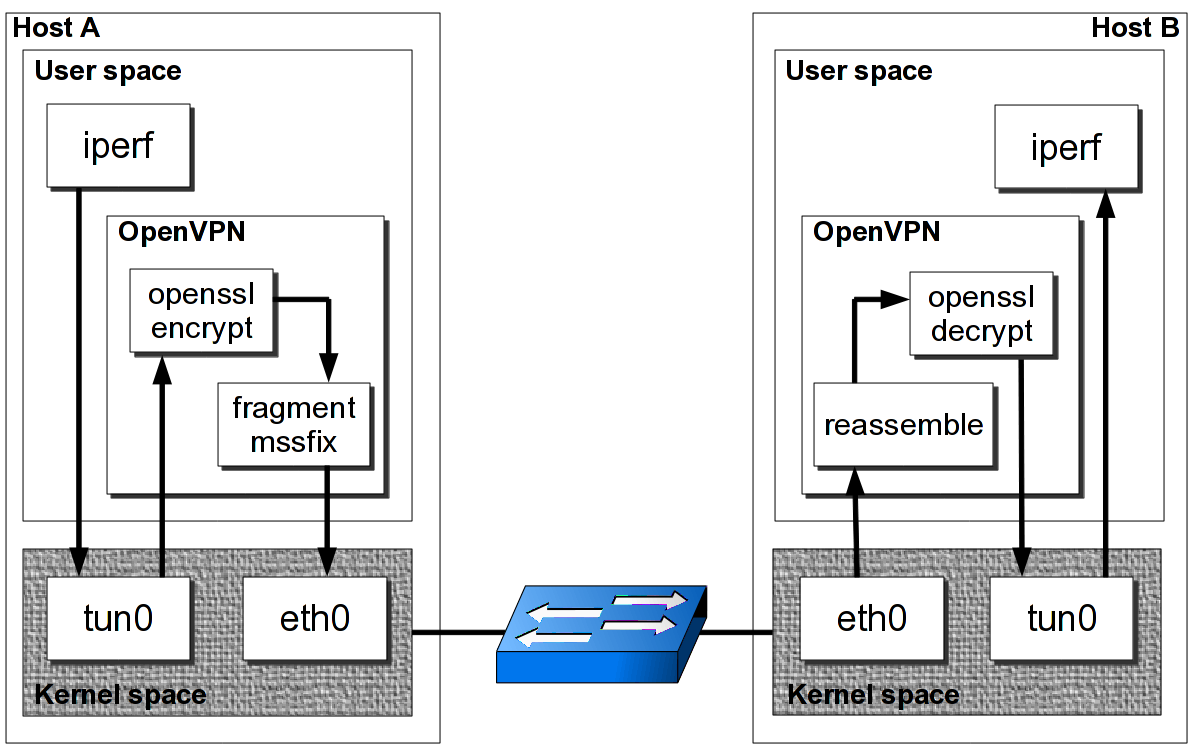
\includegraphics[width=\textwidth]{OpenVPN-packetflow}
\caption{OpenVPN packet flow as advertized on the openVPN wiki.}{}
\label{fig:openvpn-packet-flow}
\end{figure}


\subsection{OpenSSH}
% Talk about the MAC=none patch
% connection using SSL/TLS, then AES, but without fragmentation (unlike openvpn)
OpenSSH relies on an external cryptographic library for all its security operations.
Up until the version 6.7 published in october 2014, it had to be compiled against OpenSSL.
However, after the infamous security vulnerability heartbleed in april 2014, the developpers took a step to move towards LibreSSL, a fork of OpenSSL managed by OpenBSD  developers.
Still, there is no official support for any other cryptographic library.

If OpenSSH does support most of OpenSSL ciphers by default, it takes some liberties such as disabling the CBC encryption mode and removing the support of no MAC during a transmission.

\noindent The first liberty is a laste\footnote{A vulnerability note as been issued by Carnegie Mellon University Computer Emergency Response Team in early 2009 (last revision)~\cite{CERT2009}, in response to a research of University of London~\cite{Albrecht:2009} presenting a plaintext-recovering attack against SSH when CBC mode is used, but the OpenSSH update took only place in october 2014.}.
Even if it is not recommended, the user can still enable this mode by explicitly configuring it in the \texttt{sshd\_config} options.

\noindent The second liberty has been taken to prevent the user to strip himself from data authenticity and integrity.
However, in the case of testing and benchmarking, leaving the MAC behind can be interresting, especially if it is not offloaded in hardware such as the encryption in our case.
In order to add this feature to OpenSSH, we wrote a patch to apply on OpenSSH 6.7, available in appendix~\cite{chap:openssh-patch}.




\subsection{OpenSSL}

Offers an high-level interface called EVP to be used by other applications.


It is to be noted that the present work uses an implementation with all the debug flags activated.
Figure~\ref{fig:openssl-speed-dbg-on-off} shows that if it does have an impact on the performance, it is minimal: in the worst case of the benchmark, the throughput drops only by 2.4\%.
Moreover, the benchmark maximizes this difference by doing only OpenSSL operations.
When OpenSSL will have to share the CPU with other applications, the loss will be even less noticeable.
\begin{figure}[ht]
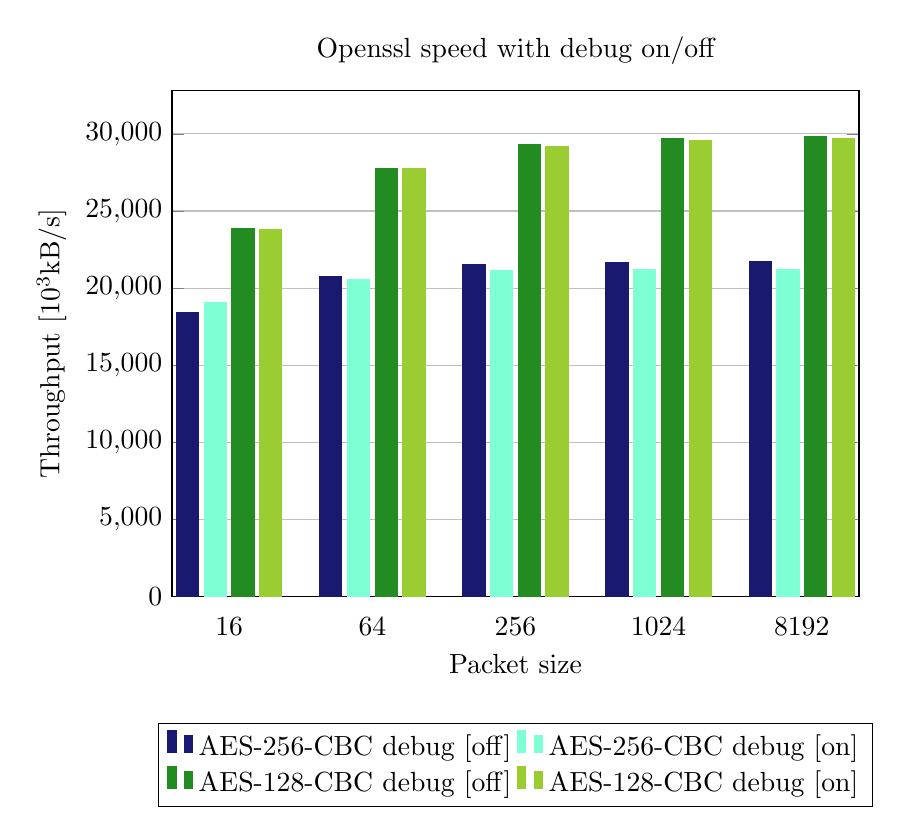
\begin{tikzpicture}
\begin{axis}[
		title = {Openssl speed with debug on/off},
        width  = 0.85*\textwidth,
        height = 8cm,
        major x tick style = transparent,
        ybar,
        bar width=8pt,
        ymajorgrids = true,
        ylabel = {Throughput [$10^3$kB/s]},
        xlabel = {Packet size},
        ymin=0,
        symbolic x coords={16,64,256,1024,8192},
        xtick = data,
        scaled y ticks = false,%Disable the *10^4 exponent applied to all y axis markings.
        legend style={at={(0.5,-0.25)},	anchor=north,legend columns=2},
        enlarge x limits=0.1,
    ]
\addplot[style={MidnightBlue,fill=MidnightBlue,mark=none}]
	coordinates {(16,18400.60) (64,20750.61) (256,21507.33) (1024,21681.15) (8192,21725.18)};
	\label{aes-256-cbc-dbg-off}

\addplot[style={Aquamarine,fill=Aquamarine,mark=none}]
	coordinates {(16,19091.65) (64,20579.24) (256,21106.60) (1024,21216.26) (8192,21203.63)};
	\label{aes-256-cbc-dbg-on}

\addplot[style={ForestGreen,fill=ForestGreen,mark=none}]
	coordinates {(16,23882.41) (64,27781.80) (256,29285.63) (1024,29692.25) (8192,29807.96)};
	\label{aes-128-cbc-dbg-off}

\addplot[style={YellowGreen,fill=YellowGreen,mark=none}]
	coordinates {(16,23806.36) (64,27728.96) (256,29181.70) (1024,29573.46) (8192,29687.81)};
	\label{aes-128-cbc-dbg-on}

\legend{AES-256-CBC debug [off], AES-256-CBC debug [on], AES-128-CBC debug [off], AES-128-CBC debug [on]}
\end{axis}
\end{tikzpicture}
\caption{OpenSSL debugging benchmark}{Software benchmark of Openssl speed for AES mode CBC, with 128- and 256-bit keys, debugging flags (de)activated at compilation (\texttt{-fno-inline -g -marm}). The throughput difference ranges from 0.2\% and 2.4\% , and is more marked for larger keysize, as more debugging data needs to be generated.}
\label{fig:openssl-speed-dbg-on-off}
\end{figure}

% Talk about the assembly implementation, maybe show the difference in an appendice with the C implementation. Not /that/ interresting.


\subsection{Strongswan}
% TODO talk about IKE and SA management
Strongswan is a full implementation of IPSec relying on the kernel drivers for the networking part, on the crypto API for the cryptographic part, and on user space crypto libraries for the connection negociation.
An other popular implementation is ipsec-tools, but its development lags behind modern Linux and is not up-to-date with the 3.14 Linux kernel headers, making its cross-compilation painfull.
%Use strongswan 5.3.0
Strongswan as two advantages: it has a tremendous and exhaustive documentation, and its uer interface is straightforward.
Once configured, a simple \texttt{ipsec start \&\& ipsec up <connection>} on both sides is enough to create a ready to use VPN.

The figure~\ref{fig:ipsec-workflow} illustrates the workflow of Alice communicating with Bob via an IPSec ESP tunnel.
The XFRM, read ``transform", framework is implementing IPSec and handles the incomming and outgoing packets for established VPNs~\cite{rosen2014}.
Its name comes from the fact that the kernel transforms packet frames to incorporate IPSec security.
Depending on the configuration, XFRM uses the AH or ESP kernel module, which in turn calls the crypto API to encrypt and/or sign the IP packet.

We can also clearly see one of the main advantages of IPSec: it works in the kernel space.
Since it does not require a virtual network interface like OpenVPN, the only transfer between the user/kernel space happens when the former wishes to send a packet on the network, passing it to the later -- or \textit{vice versa} for incomming packets.

\begin{figure}[ht]
\Large
\resizebox{\linewidth}{!}{%
% Graphic for TeX using PGF
% Title: /home/para/documents/polytech2015/MA2/Master_thesis/master_thesis/ipsec-transfer.dia
% Creator: Dia v0.97.3
% CreationDate: Sat May 16 13:42:52 2015
% For: para
% \usepackage{tikz}
% The following commands are not supported in PSTricks at present
% We define them conditionally, so when they are implemented,
% this pgf file will use them.
\ifx\du\undefined
  \newlength{\du}
\fi
\setlength{\du}{15\unitlength}
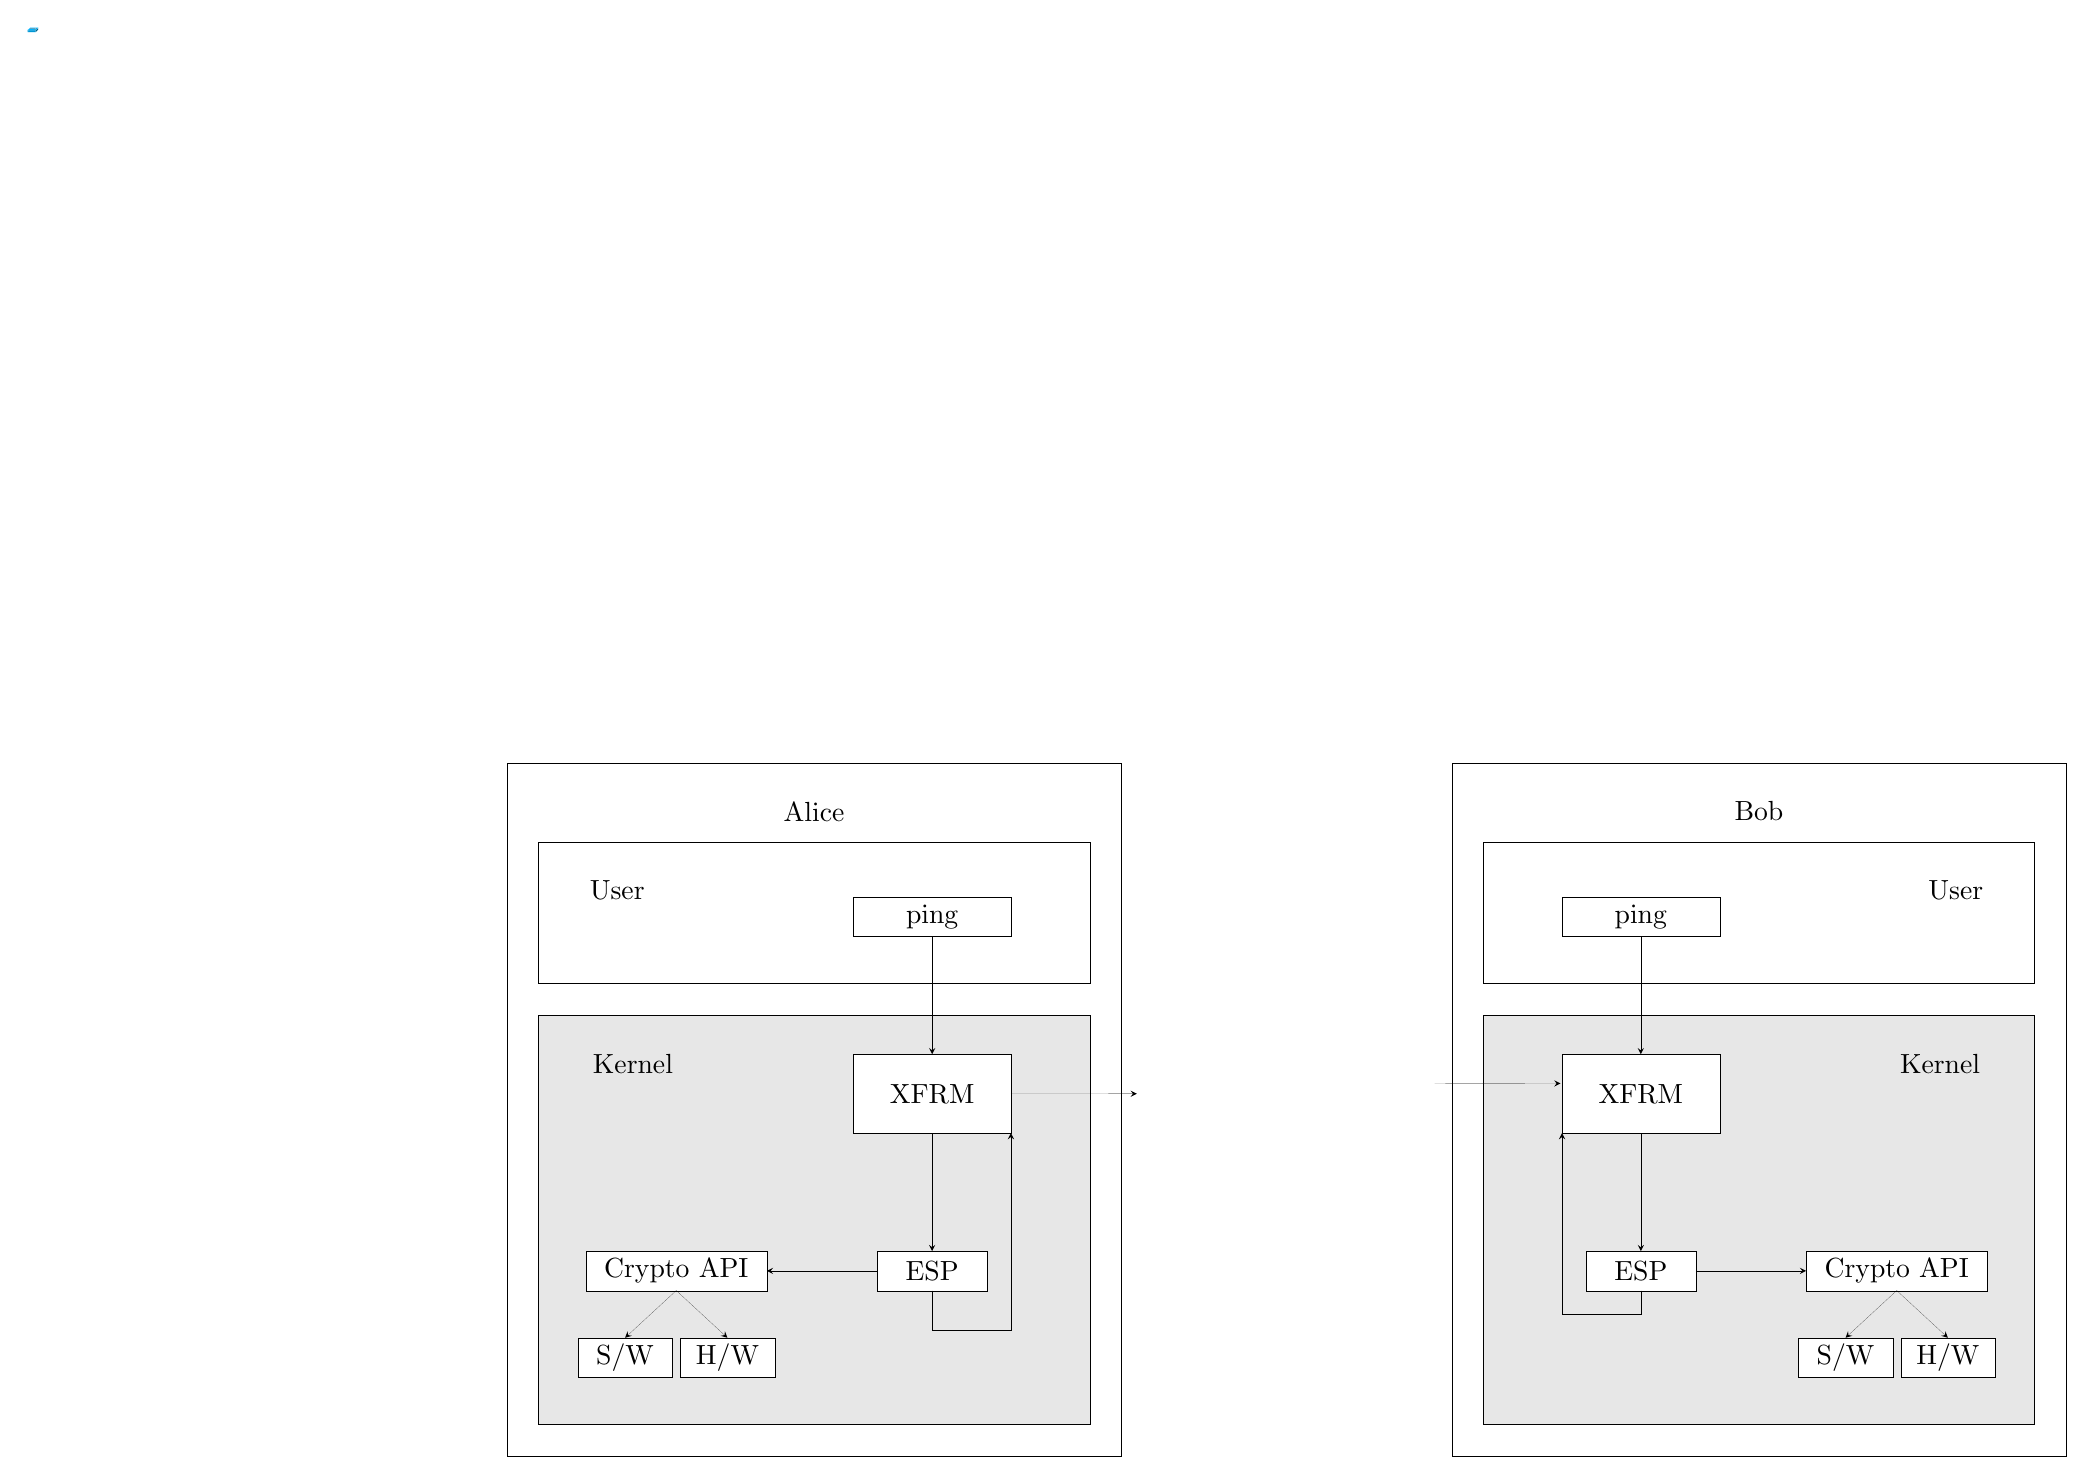
\begin{tikzpicture}
\pgftransformxscale{1.000000}
\pgftransformyscale{-1.000000}
\definecolor{dialinecolor}{rgb}{0.000000, 0.000000, 0.000000}
\pgfsetstrokecolor{dialinecolor}
\definecolor{dialinecolor}{rgb}{1.000000, 1.000000, 1.000000}
\pgfsetfillcolor{dialinecolor}
\pgfsetlinewidth{0.050000\du}
\pgfsetdash{}{0pt}
\pgfsetdash{}{0pt}
\pgfsetmiterjoin
\definecolor{dialinecolor}{rgb}{1.000000, 1.000000, 1.000000}
\pgfsetfillcolor{dialinecolor}
\fill (6.600000\du,9.800000\du)--(6.600000\du,10.800000\du)--(14.400000\du,10.800000\du)--(14.400000\du,9.800000\du)--cycle;
\definecolor{dialinecolor}{rgb}{0.000000, 0.000000, 0.000000}
\pgfsetstrokecolor{dialinecolor}
\draw (6.600000\du,9.800000\du)--(6.600000\du,10.800000\du)--(14.400000\du,10.800000\du)--(14.400000\du,9.800000\du)--cycle;
\pgfsetlinewidth{0.050000\du}
\pgfsetdash{}{0pt}
\pgfsetdash{}{0pt}
\pgfsetmiterjoin
\definecolor{dialinecolor}{rgb}{1.000000, 1.000000, 1.000000}
\pgfsetfillcolor{dialinecolor}
\fill (6.600000\du,9.800000\du)--(6.600000\du,18.600000\du)--(14.400000\du,18.600000\du)--(14.400000\du,9.800000\du)--cycle;
\definecolor{dialinecolor}{rgb}{0.000000, 0.000000, 0.000000}
\pgfsetstrokecolor{dialinecolor}
\draw (6.600000\du,9.800000\du)--(6.600000\du,18.600000\du)--(14.400000\du,18.600000\du)--(14.400000\du,9.800000\du)--cycle;
% setfont left to latex
\definecolor{dialinecolor}{rgb}{0.000000, 0.000000, 0.000000}
\pgfsetstrokecolor{dialinecolor}
\node at (10.500000\du,10.416250\du){Alice};
\pgfsetlinewidth{0.050000\du}
\pgfsetdash{}{0pt}
\pgfsetdash{}{0pt}
\pgfsetmiterjoin
\definecolor{dialinecolor}{rgb}{1.000000, 1.000000, 1.000000}
\pgfsetfillcolor{dialinecolor}
\fill (18.600000\du,9.800000\du)--(18.600000\du,10.800000\du)--(26.400000\du,10.800000\du)--(26.400000\du,9.800000\du)--cycle;
\definecolor{dialinecolor}{rgb}{0.000000, 0.000000, 0.000000}
\pgfsetstrokecolor{dialinecolor}
\draw (18.600000\du,9.800000\du)--(18.600000\du,10.800000\du)--(26.400000\du,10.800000\du)--(26.400000\du,9.800000\du)--cycle;
\pgfsetlinewidth{0.050000\du}
\pgfsetdash{}{0pt}
\pgfsetdash{}{0pt}
\pgfsetmiterjoin
\definecolor{dialinecolor}{rgb}{1.000000, 1.000000, 1.000000}
\pgfsetfillcolor{dialinecolor}
\fill (18.600000\du,9.800000\du)--(18.600000\du,18.600000\du)--(26.400000\du,18.600000\du)--(26.400000\du,9.800000\du)--cycle;
\definecolor{dialinecolor}{rgb}{0.000000, 0.000000, 0.000000}
\pgfsetstrokecolor{dialinecolor}
\draw (18.600000\du,9.800000\du)--(18.600000\du,18.600000\du)--(26.400000\du,18.600000\du)--(26.400000\du,9.800000\du)--cycle;
% setfont left to latex
\definecolor{dialinecolor}{rgb}{0.000000, 0.000000, 0.000000}
\pgfsetstrokecolor{dialinecolor}
\node at (22.500000\du,10.411344\du){Bob};
\pgfsetlinewidth{0.050000\du}
\pgfsetdash{}{0pt}
\pgfsetdash{}{0pt}
\pgfsetmiterjoin
\definecolor{dialinecolor}{rgb}{1.000000, 1.000000, 1.000000}
\pgfsetfillcolor{dialinecolor}
\fill (7.000000\du,13.000000\du)--(7.000000\du,14.000000\du)--(9.400000\du,14.000000\du)--(9.400000\du,13.000000\du)--cycle;
\definecolor{dialinecolor}{rgb}{0.000000, 0.000000, 0.000000}
\pgfsetstrokecolor{dialinecolor}
\draw (7.000000\du,13.000000\du)--(7.000000\du,14.000000\du)--(9.400000\du,14.000000\du)--(9.400000\du,13.000000\du)--cycle;
\pgfsetlinewidth{0.050000\du}
\pgfsetdash{}{0pt}
\pgfsetdash{}{0pt}
\pgfsetmiterjoin
\definecolor{dialinecolor}{rgb}{0.905882, 0.905882, 0.905882}
\pgfsetfillcolor{dialinecolor}
\fill (7.000000\du,13.000000\du)--(7.000000\du,18.200000\du)--(14.000000\du,18.200000\du)--(14.000000\du,13.000000\du)--cycle;
\definecolor{dialinecolor}{rgb}{0.000000, 0.000000, 0.000000}
\pgfsetstrokecolor{dialinecolor}
\draw (7.000000\du,13.000000\du)--(7.000000\du,18.200000\du)--(14.000000\du,18.200000\du)--(14.000000\du,13.000000\du)--cycle;
\pgfsetlinewidth{0.000000\du}
\pgfsetdash{}{0pt}
\pgfsetdash{}{0pt}
\pgfsetmiterjoin
\definecolor{dialinecolor}{rgb}{1.000000, 1.000000, 1.000000}
\pgfsetfillcolor{dialinecolor}
\fill (7.000000\du,10.800000\du)--(7.000000\du,11.800000\du)--(9.000000\du,11.800000\du)--(9.000000\du,10.800000\du)--cycle;
\definecolor{dialinecolor}{rgb}{1.000000, 1.000000, 1.000000}
\pgfsetstrokecolor{dialinecolor}
\draw (7.000000\du,10.800000\du)--(7.000000\du,11.800000\du)--(9.000000\du,11.800000\du)--(9.000000\du,10.800000\du)--cycle;
\pgfsetlinewidth{0.050000\du}
\pgfsetdash{}{0pt}
\pgfsetdash{}{0pt}
\pgfsetmiterjoin
\definecolor{dialinecolor}{rgb}{1.000000, 1.000000, 1.000000}
\pgfsetfillcolor{dialinecolor}
\fill (7.000000\du,10.800000\du)--(7.000000\du,12.600000\du)--(14.000000\du,12.600000\du)--(14.000000\du,10.800000\du)--cycle;
\definecolor{dialinecolor}{rgb}{0.000000, 0.000000, 0.000000}
\pgfsetstrokecolor{dialinecolor}
\draw (7.000000\du,10.800000\du)--(7.000000\du,12.600000\du)--(14.000000\du,12.600000\du)--(14.000000\du,10.800000\du)--cycle;
% setfont left to latex
\definecolor{dialinecolor}{rgb}{0.000000, 0.000000, 0.000000}
\pgfsetstrokecolor{dialinecolor}
\node at (8.000000\du,11.416250\du){User};
% setfont left to latex
\definecolor{dialinecolor}{rgb}{0.000000, 0.000000, 0.000000}
\pgfsetstrokecolor{dialinecolor}
\node at (8.200000\du,13.616250\du){Kernel};
\pgfsetlinewidth{0.050000\du}
\pgfsetdash{}{0pt}
\pgfsetdash{}{0pt}
\pgfsetmiterjoin
\definecolor{dialinecolor}{rgb}{1.000000, 1.000000, 1.000000}
\pgfsetfillcolor{dialinecolor}
\fill (23.600000\du,13.000000\du)--(23.600000\du,14.000000\du)--(26.000000\du,14.000000\du)--(26.000000\du,13.000000\du)--cycle;
\definecolor{dialinecolor}{rgb}{0.000000, 0.000000, 0.000000}
\pgfsetstrokecolor{dialinecolor}
\draw (23.600000\du,13.000000\du)--(23.600000\du,14.000000\du)--(26.000000\du,14.000000\du)--(26.000000\du,13.000000\du)--cycle;
\pgfsetlinewidth{0.050000\du}
\pgfsetdash{}{0pt}
\pgfsetdash{}{0pt}
\pgfsetmiterjoin
\definecolor{dialinecolor}{rgb}{0.905882, 0.905882, 0.905882}
\pgfsetfillcolor{dialinecolor}
\fill (19.000000\du,13.000000\du)--(19.000000\du,18.200000\du)--(26.000000\du,18.200000\du)--(26.000000\du,13.000000\du)--cycle;
\definecolor{dialinecolor}{rgb}{0.000000, 0.000000, 0.000000}
\pgfsetstrokecolor{dialinecolor}
\draw (19.000000\du,13.000000\du)--(19.000000\du,18.200000\du)--(26.000000\du,18.200000\du)--(26.000000\du,13.000000\du)--cycle;
\pgfsetlinewidth{0.000000\du}
\pgfsetdash{}{0pt}
\pgfsetdash{}{0pt}
\pgfsetmiterjoin
\definecolor{dialinecolor}{rgb}{1.000000, 1.000000, 1.000000}
\pgfsetfillcolor{dialinecolor}
\fill (24.000000\du,10.800000\du)--(24.000000\du,11.800000\du)--(26.000000\du,11.800000\du)--(26.000000\du,10.800000\du)--cycle;
\definecolor{dialinecolor}{rgb}{1.000000, 1.000000, 1.000000}
\pgfsetstrokecolor{dialinecolor}
\draw (24.000000\du,10.800000\du)--(24.000000\du,11.800000\du)--(26.000000\du,11.800000\du)--(26.000000\du,10.800000\du)--cycle;
\pgfsetlinewidth{0.050000\du}
\pgfsetdash{}{0pt}
\pgfsetdash{}{0pt}
\pgfsetmiterjoin
\definecolor{dialinecolor}{rgb}{1.000000, 1.000000, 1.000000}
\pgfsetfillcolor{dialinecolor}
\fill (19.000000\du,10.800000\du)--(19.000000\du,12.600000\du)--(26.000000\du,12.600000\du)--(26.000000\du,10.800000\du)--cycle;
\definecolor{dialinecolor}{rgb}{0.000000, 0.000000, 0.000000}
\pgfsetstrokecolor{dialinecolor}
\draw (19.000000\du,10.800000\du)--(19.000000\du,12.600000\du)--(26.000000\du,12.600000\du)--(26.000000\du,10.800000\du)--cycle;
% setfont left to latex
\definecolor{dialinecolor}{rgb}{0.000000, 0.000000, 0.000000}
\pgfsetstrokecolor{dialinecolor}
\node at (25.000000\du,11.416250\du){User};
% setfont left to latex
\definecolor{dialinecolor}{rgb}{0.000000, 0.000000, 0.000000}
\pgfsetstrokecolor{dialinecolor}
\node at (24.800000\du,13.616250\du){Kernel};
\pgfsetlinewidth{0.020000\du}
\pgfsetdash{}{0pt}
\pgfsetdash{}{0pt}
\pgfsetbuttcap
\pgfsetmiterjoin
\pgfsetlinewidth{0.000200\du}
\pgfsetbuttcap
\pgfsetmiterjoin
\pgfsetdash{}{0pt}
\definecolor{dialinecolor}{rgb}{0.000000, 0.588235, 0.831373}
\pgfsetfillcolor{dialinecolor}
\pgfpathmoveto{\pgfpoint{14.600000\du}{14.000632\du}}
\pgfpathlineto{\pgfpoint{14.600000\du}{14.731085\du}}
\pgfpathlineto{\pgfpoint{17.488279\du}{14.731085\du}}
\pgfpathlineto{\pgfpoint{17.488279\du}{14.000632\du}}
\pgfpathlineto{\pgfpoint{14.600000\du}{14.000632\du}}
\pgfusepath{fill}
\pgfsetbuttcap
\pgfsetmiterjoin
\pgfsetdash{}{0pt}
\definecolor{dialinecolor}{rgb}{0.666667, 0.901961, 1.000000}
\pgfsetstrokecolor{dialinecolor}
\pgfpathmoveto{\pgfpoint{14.600000\du}{14.000632\du}}
\pgfpathlineto{\pgfpoint{14.600000\du}{14.731085\du}}
\pgfpathlineto{\pgfpoint{17.488279\du}{14.731085\du}}
\pgfpathlineto{\pgfpoint{17.488279\du}{14.000632\du}}
\pgfpathlineto{\pgfpoint{14.600000\du}{14.000632\du}}
\pgfusepath{stroke}
\pgfsetbuttcap
\pgfsetmiterjoin
\pgfsetdash{}{0pt}
\definecolor{dialinecolor}{rgb}{0.000000, 0.352941, 0.501961}
\pgfsetfillcolor{dialinecolor}
\pgfpathmoveto{\pgfpoint{17.488279\du}{14.000632\du}}
\pgfpathlineto{\pgfpoint{18.381785\du}{13.140000\du}}
\pgfpathlineto{\pgfpoint{18.381785\du}{13.871110\du}}
\pgfpathlineto{\pgfpoint{17.488279\du}{14.731085\du}}
\pgfpathlineto{\pgfpoint{17.488279\du}{14.000632\du}}
\pgfusepath{fill}
\pgfsetbuttcap
\pgfsetmiterjoin
\pgfsetdash{}{0pt}
\definecolor{dialinecolor}{rgb}{0.666667, 0.901961, 1.000000}
\pgfsetstrokecolor{dialinecolor}
\pgfpathmoveto{\pgfpoint{17.488279\du}{14.000632\du}}
\pgfpathlineto{\pgfpoint{18.381785\du}{13.140000\du}}
\pgfpathlineto{\pgfpoint{18.381785\du}{13.871110\du}}
\pgfpathlineto{\pgfpoint{17.488279\du}{14.731085\du}}
\pgfpathlineto{\pgfpoint{17.488279\du}{14.000632\du}}
\pgfusepath{stroke}
\pgfsetbuttcap
\pgfsetmiterjoin
\pgfsetdash{}{0pt}
\definecolor{dialinecolor}{rgb}{0.000000, 0.705882, 1.000000}
\pgfsetfillcolor{dialinecolor}
\pgfpathmoveto{\pgfpoint{17.488279\du}{14.000632\du}}
\pgfpathlineto{\pgfpoint{18.381785\du}{13.140000\du}}
\pgfpathlineto{\pgfpoint{15.492848\du}{13.140000\du}}
\pgfpathlineto{\pgfpoint{14.600000\du}{14.000632\du}}
\pgfpathlineto{\pgfpoint{17.488279\du}{14.000632\du}}
\pgfusepath{fill}
\pgfsetbuttcap
\pgfsetmiterjoin
\pgfsetdash{}{0pt}
\definecolor{dialinecolor}{rgb}{0.666667, 0.901961, 1.000000}
\pgfsetstrokecolor{dialinecolor}
\pgfpathmoveto{\pgfpoint{17.488279\du}{14.000632\du}}
\pgfpathlineto{\pgfpoint{18.381785\du}{13.140000\du}}
\pgfpathlineto{\pgfpoint{15.492848\du}{13.140000\du}}
\pgfpathlineto{\pgfpoint{14.600000\du}{14.000632\du}}
\pgfpathlineto{\pgfpoint{17.488279\du}{14.000632\du}}
\pgfusepath{stroke}
\pgfsetbuttcap
\pgfsetmiterjoin
\pgfsetdash{}{0pt}
\definecolor{dialinecolor}{rgb}{0.000000, 0.000000, 0.000000}
\pgfsetfillcolor{dialinecolor}
\pgfpathmoveto{\pgfpoint{15.544789\du}{13.452300\du}}
\pgfpathlineto{\pgfpoint{15.388968\du}{13.608778\du}}
\pgfpathlineto{\pgfpoint{17.122067\du}{13.608778\du}}
\pgfpathlineto{\pgfpoint{16.989257\du}{13.739615\du}}
\pgfpathlineto{\pgfpoint{17.724970\du}{13.556838\du}}
\pgfpathlineto{\pgfpoint{17.358100\du}{13.374060\du}}
\pgfpathlineto{\pgfpoint{17.278545\du}{13.452300\du}}
\pgfpathlineto{\pgfpoint{15.544789\du}{13.452300\du}}
\pgfusepath{fill}
\pgfsetbuttcap
\pgfsetmiterjoin
\pgfsetdash{}{0pt}
\definecolor{dialinecolor}{rgb}{1.000000, 1.000000, 1.000000}
\pgfsetfillcolor{dialinecolor}
\pgfpathmoveto{\pgfpoint{15.571088\du}{13.478599\du}}
\pgfpathlineto{\pgfpoint{15.413294\du}{13.608778\du}}
\pgfpathlineto{\pgfpoint{17.147051\du}{13.608778\du}}
\pgfpathlineto{\pgfpoint{17.015556\du}{13.739615\du}}
\pgfpathlineto{\pgfpoint{17.724970\du}{13.583794\du}}
\pgfpathlineto{\pgfpoint{17.383084\du}{13.401017\du}}
\pgfpathlineto{\pgfpoint{17.278545\du}{13.478599\du}}
\pgfpathlineto{\pgfpoint{15.571088\du}{13.478599\du}}
\pgfusepath{fill}
\pgfsetlinewidth{0.020000\du}
\pgfsetdash{}{0pt}
\pgfsetdash{}{0pt}
\pgfsetmiterjoin
\definecolor{dialinecolor}{rgb}{1.000000, 1.000000, 1.000000}
\pgfsetfillcolor{dialinecolor}
\fill (11.000000\du,11.500000\du)--(11.000000\du,12.000000\du)--(13.000000\du,12.000000\du)--(13.000000\du,11.500000\du)--cycle;
\definecolor{dialinecolor}{rgb}{0.000000, 0.000000, 0.000000}
\pgfsetstrokecolor{dialinecolor}
\draw (11.000000\du,11.500000\du)--(11.000000\du,12.000000\du)--(13.000000\du,12.000000\du)--(13.000000\du,11.500000\du)--cycle;
% setfont left to latex
\definecolor{dialinecolor}{rgb}{0.000000, 0.000000, 0.000000}
\pgfsetstrokecolor{dialinecolor}
\node at (12.000000\du,11.750000\du){ping};
\pgfsetlinewidth{0.020000\du}
\pgfsetdash{}{0pt}
\pgfsetdash{}{0pt}
\pgfsetmiterjoin
\definecolor{dialinecolor}{rgb}{1.000000, 1.000000, 1.000000}
\pgfsetfillcolor{dialinecolor}
\fill (11.000000\du,13.500000\du)--(11.000000\du,14.500000\du)--(13.000000\du,14.500000\du)--(13.000000\du,13.500000\du)--cycle;
\definecolor{dialinecolor}{rgb}{0.000000, 0.000000, 0.000000}
\pgfsetstrokecolor{dialinecolor}
\draw (11.000000\du,13.500000\du)--(11.000000\du,14.500000\du)--(13.000000\du,14.500000\du)--(13.000000\du,13.500000\du)--cycle;
% setfont left to latex
\definecolor{dialinecolor}{rgb}{0.000000, 0.000000, 0.000000}
\pgfsetstrokecolor{dialinecolor}
\node at (12.000000\du,14.000000\du){XFRM};
\pgfsetlinewidth{0.020000\du}
\pgfsetdash{}{0pt}
\pgfsetdash{}{0pt}
\pgfsetmiterjoin
\definecolor{dialinecolor}{rgb}{1.000000, 1.000000, 1.000000}
\pgfsetfillcolor{dialinecolor}
\fill (11.300000\du,16.000000\du)--(11.300000\du,16.500000\du)--(12.700000\du,16.500000\du)--(12.700000\du,16.000000\du)--cycle;
\definecolor{dialinecolor}{rgb}{0.000000, 0.000000, 0.000000}
\pgfsetstrokecolor{dialinecolor}
\draw (11.300000\du,16.000000\du)--(11.300000\du,16.500000\du)--(12.700000\du,16.500000\du)--(12.700000\du,16.000000\du)--cycle;
% setfont left to latex
\definecolor{dialinecolor}{rgb}{0.000000, 0.000000, 0.000000}
\pgfsetstrokecolor{dialinecolor}
\node at (12.000000\du,16.250000\du){ESP};
\pgfsetlinewidth{0.020000\du}
\pgfsetdash{}{0pt}
\pgfsetdash{}{0pt}
\pgfsetmiterjoin
\definecolor{dialinecolor}{rgb}{1.000000, 1.000000, 1.000000}
\pgfsetfillcolor{dialinecolor}
\fill (7.600000\du,16.000000\du)--(7.600000\du,16.500000\du)--(9.900000\du,16.500000\du)--(9.900000\du,16.000000\du)--cycle;
\definecolor{dialinecolor}{rgb}{0.000000, 0.000000, 0.000000}
\pgfsetstrokecolor{dialinecolor}
\draw (7.600000\du,16.000000\du)--(7.600000\du,16.500000\du)--(9.900000\du,16.500000\du)--(9.900000\du,16.000000\du)--cycle;
% setfont left to latex
\definecolor{dialinecolor}{rgb}{0.000000, 0.000000, 0.000000}
\pgfsetstrokecolor{dialinecolor}
\node at (8.750000\du,16.250000\du){Crypto API};
\pgfsetlinewidth{0.020000\du}
\pgfsetdash{}{0pt}
\pgfsetdash{}{0pt}
\pgfsetmiterjoin
\definecolor{dialinecolor}{rgb}{1.000000, 1.000000, 1.000000}
\pgfsetfillcolor{dialinecolor}
\fill (7.500000\du,17.100000\du)--(7.500000\du,17.600000\du)--(8.700000\du,17.600000\du)--(8.700000\du,17.100000\du)--cycle;
\definecolor{dialinecolor}{rgb}{0.000000, 0.000000, 0.000000}
\pgfsetstrokecolor{dialinecolor}
\draw (7.500000\du,17.100000\du)--(7.500000\du,17.600000\du)--(8.700000\du,17.600000\du)--(8.700000\du,17.100000\du)--cycle;
% setfont left to latex
\definecolor{dialinecolor}{rgb}{0.000000, 0.000000, 0.000000}
\pgfsetstrokecolor{dialinecolor}
\node at (8.100000\du,17.350000\du){S/W};
\pgfsetlinewidth{0.020000\du}
\pgfsetdash{}{0pt}
\pgfsetdash{}{0pt}
\pgfsetmiterjoin
\definecolor{dialinecolor}{rgb}{1.000000, 1.000000, 1.000000}
\pgfsetfillcolor{dialinecolor}
\fill (8.800000\du,17.100000\du)--(8.800000\du,17.600000\du)--(10.000000\du,17.600000\du)--(10.000000\du,17.100000\du)--cycle;
\definecolor{dialinecolor}{rgb}{0.000000, 0.000000, 0.000000}
\pgfsetstrokecolor{dialinecolor}
\draw (8.800000\du,17.100000\du)--(8.800000\du,17.600000\du)--(10.000000\du,17.600000\du)--(10.000000\du,17.100000\du)--cycle;
% setfont left to latex
\definecolor{dialinecolor}{rgb}{0.000000, 0.000000, 0.000000}
\pgfsetstrokecolor{dialinecolor}
\node at (9.400000\du,17.350000\du){H/W};
\pgfsetlinewidth{0.020000\du}
\pgfsetdash{}{0pt}
\pgfsetdash{}{0pt}
\pgfsetbuttcap
{
\definecolor{dialinecolor}{rgb}{0.000000, 0.000000, 0.000000}
\pgfsetfillcolor{dialinecolor}
% was here!!!
\pgfsetarrowsend{stealth}
\definecolor{dialinecolor}{rgb}{0.000000, 0.000000, 0.000000}
\pgfsetstrokecolor{dialinecolor}
\draw (12.000000\du,14.500000\du)--(12.000000\du,16.000000\du);
}
\pgfsetlinewidth{0.020000\du}
\pgfsetdash{}{0pt}
\pgfsetdash{}{0pt}
\pgfsetbuttcap
{
\definecolor{dialinecolor}{rgb}{0.000000, 0.000000, 0.000000}
\pgfsetfillcolor{dialinecolor}
% was here!!!
\pgfsetarrowsend{stealth}
\definecolor{dialinecolor}{rgb}{0.000000, 0.000000, 0.000000}
\pgfsetstrokecolor{dialinecolor}
\draw (11.300000\du,16.250000\du)--(9.900000\du,16.250000\du);
}
\pgfsetlinewidth{0.020000\du}
\pgfsetdash{}{0pt}
\pgfsetdash{}{0pt}
\pgfsetbuttcap
{
\definecolor{dialinecolor}{rgb}{0.000000, 0.000000, 0.000000}
\pgfsetfillcolor{dialinecolor}
% was here!!!
\pgfsetarrowsend{stealth}
\definecolor{dialinecolor}{rgb}{0.000000, 0.000000, 0.000000}
\pgfsetstrokecolor{dialinecolor}
\draw (8.750000\du,16.500000\du)--(8.100000\du,17.100000\du);
}
\pgfsetlinewidth{0.020000\du}
\pgfsetdash{}{0pt}
\pgfsetdash{}{0pt}
\pgfsetbuttcap
{
\definecolor{dialinecolor}{rgb}{0.000000, 0.000000, 0.000000}
\pgfsetfillcolor{dialinecolor}
% was here!!!
\pgfsetarrowsend{stealth}
\definecolor{dialinecolor}{rgb}{0.000000, 0.000000, 0.000000}
\pgfsetstrokecolor{dialinecolor}
\draw (8.750000\du,16.500000\du)--(9.400000\du,17.100000\du);
}
\pgfsetlinewidth{0.020000\du}
\pgfsetdash{}{0pt}
\pgfsetdash{}{0pt}
\pgfsetbuttcap
{
\definecolor{dialinecolor}{rgb}{0.000000, 0.000000, 0.000000}
\pgfsetfillcolor{dialinecolor}
% was here!!!
\pgfsetarrowsend{stealth}
\definecolor{dialinecolor}{rgb}{0.000000, 0.000000, 0.000000}
\pgfsetstrokecolor{dialinecolor}
\draw (13.000000\du,14.000000\du)--(14.600000\du,14.000632\du);
}
\pgfsetlinewidth{0.020000\du}
\pgfsetdash{}{0pt}
\pgfsetdash{}{0pt}
\pgfsetbuttcap
{
\definecolor{dialinecolor}{rgb}{0.000000, 0.000000, 0.000000}
\pgfsetfillcolor{dialinecolor}
% was here!!!
\pgfsetarrowsend{stealth}
\definecolor{dialinecolor}{rgb}{0.000000, 0.000000, 0.000000}
\pgfsetstrokecolor{dialinecolor}
\draw (12.000000\du,12.000000\du)--(12.000000\du,13.500000\du);
}
\pgfsetlinewidth{0.020000\du}
\pgfsetdash{}{0pt}
\pgfsetdash{}{0pt}
\pgfsetmiterjoin
\pgfsetbuttcap
{
\definecolor{dialinecolor}{rgb}{0.000000, 0.000000, 0.000000}
\pgfsetfillcolor{dialinecolor}
% was here!!!
\pgfsetarrowsend{stealth}
{\pgfsetcornersarced{\pgfpoint{0.000000\du}{0.000000\du}}\definecolor{dialinecolor}{rgb}{0.000000, 0.000000, 0.000000}
\pgfsetstrokecolor{dialinecolor}
\draw (12.000000\du,16.500000\du)--(12.000000\du,17.000000\du)--(13.000000\du,17.000000\du)--(13.000000\du,14.500000\du);
}}
\pgfsetlinewidth{0.020000\du}
\pgfsetdash{}{0pt}
\pgfsetdash{}{0pt}
\pgfsetmiterjoin
\definecolor{dialinecolor}{rgb}{1.000000, 1.000000, 1.000000}
\pgfsetfillcolor{dialinecolor}
\fill (20.000000\du,11.500000\du)--(20.000000\du,12.000000\du)--(22.000000\du,12.000000\du)--(22.000000\du,11.500000\du)--cycle;
\definecolor{dialinecolor}{rgb}{0.000000, 0.000000, 0.000000}
\pgfsetstrokecolor{dialinecolor}
\draw (20.000000\du,11.500000\du)--(20.000000\du,12.000000\du)--(22.000000\du,12.000000\du)--(22.000000\du,11.500000\du)--cycle;
% setfont left to latex
\definecolor{dialinecolor}{rgb}{0.000000, 0.000000, 0.000000}
\pgfsetstrokecolor{dialinecolor}
\node at (21.000000\du,11.750000\du){ping};
\pgfsetlinewidth{0.020000\du}
\pgfsetdash{}{0pt}
\pgfsetdash{}{0pt}
\pgfsetmiterjoin
\definecolor{dialinecolor}{rgb}{1.000000, 1.000000, 1.000000}
\pgfsetfillcolor{dialinecolor}
\fill (20.000000\du,13.500000\du)--(20.000000\du,14.500000\du)--(22.000000\du,14.500000\du)--(22.000000\du,13.500000\du)--cycle;
\definecolor{dialinecolor}{rgb}{0.000000, 0.000000, 0.000000}
\pgfsetstrokecolor{dialinecolor}
\draw (20.000000\du,13.500000\du)--(20.000000\du,14.500000\du)--(22.000000\du,14.500000\du)--(22.000000\du,13.500000\du)--cycle;
% setfont left to latex
\definecolor{dialinecolor}{rgb}{0.000000, 0.000000, 0.000000}
\pgfsetstrokecolor{dialinecolor}
\node at (21.000000\du,14.000000\du){XFRM};
\pgfsetlinewidth{0.020000\du}
\pgfsetdash{}{0pt}
\pgfsetdash{}{0pt}
\pgfsetmiterjoin
\definecolor{dialinecolor}{rgb}{1.000000, 1.000000, 1.000000}
\pgfsetfillcolor{dialinecolor}
\fill (20.300000\du,16.000000\du)--(20.300000\du,16.500000\du)--(21.700000\du,16.500000\du)--(21.700000\du,16.000000\du)--cycle;
\definecolor{dialinecolor}{rgb}{0.000000, 0.000000, 0.000000}
\pgfsetstrokecolor{dialinecolor}
\draw (20.300000\du,16.000000\du)--(20.300000\du,16.500000\du)--(21.700000\du,16.500000\du)--(21.700000\du,16.000000\du)--cycle;
% setfont left to latex
\definecolor{dialinecolor}{rgb}{0.000000, 0.000000, 0.000000}
\pgfsetstrokecolor{dialinecolor}
\node at (21.000000\du,16.250000\du){ESP};
\pgfsetlinewidth{0.020000\du}
\pgfsetdash{}{0pt}
\pgfsetdash{}{0pt}
\pgfsetmiterjoin
\definecolor{dialinecolor}{rgb}{1.000000, 1.000000, 1.000000}
\pgfsetfillcolor{dialinecolor}
\fill (23.100000\du,16.000000\du)--(23.100000\du,16.500000\du)--(25.400000\du,16.500000\du)--(25.400000\du,16.000000\du)--cycle;
\definecolor{dialinecolor}{rgb}{0.000000, 0.000000, 0.000000}
\pgfsetstrokecolor{dialinecolor}
\draw (23.100000\du,16.000000\du)--(23.100000\du,16.500000\du)--(25.400000\du,16.500000\du)--(25.400000\du,16.000000\du)--cycle;
% setfont left to latex
\definecolor{dialinecolor}{rgb}{0.000000, 0.000000, 0.000000}
\pgfsetstrokecolor{dialinecolor}
\node at (24.250000\du,16.250000\du){Crypto API};
\pgfsetlinewidth{0.020000\du}
\pgfsetdash{}{0pt}
\pgfsetdash{}{0pt}
\pgfsetmiterjoin
\definecolor{dialinecolor}{rgb}{1.000000, 1.000000, 1.000000}
\pgfsetfillcolor{dialinecolor}
\fill (23.000000\du,17.100000\du)--(23.000000\du,17.600000\du)--(24.200000\du,17.600000\du)--(24.200000\du,17.100000\du)--cycle;
\definecolor{dialinecolor}{rgb}{0.000000, 0.000000, 0.000000}
\pgfsetstrokecolor{dialinecolor}
\draw (23.000000\du,17.100000\du)--(23.000000\du,17.600000\du)--(24.200000\du,17.600000\du)--(24.200000\du,17.100000\du)--cycle;
% setfont left to latex
\definecolor{dialinecolor}{rgb}{0.000000, 0.000000, 0.000000}
\pgfsetstrokecolor{dialinecolor}
\node at (23.600000\du,17.350000\du){S/W};
\pgfsetlinewidth{0.020000\du}
\pgfsetdash{}{0pt}
\pgfsetdash{}{0pt}
\pgfsetmiterjoin
\definecolor{dialinecolor}{rgb}{1.000000, 1.000000, 1.000000}
\pgfsetfillcolor{dialinecolor}
\fill (24.300000\du,17.100000\du)--(24.300000\du,17.600000\du)--(25.500000\du,17.600000\du)--(25.500000\du,17.100000\du)--cycle;
\definecolor{dialinecolor}{rgb}{0.000000, 0.000000, 0.000000}
\pgfsetstrokecolor{dialinecolor}
\draw (24.300000\du,17.100000\du)--(24.300000\du,17.600000\du)--(25.500000\du,17.600000\du)--(25.500000\du,17.100000\du)--cycle;
% setfont left to latex
\definecolor{dialinecolor}{rgb}{0.000000, 0.000000, 0.000000}
\pgfsetstrokecolor{dialinecolor}
\node at (24.900000\du,17.350000\du){H/W};
\pgfsetlinewidth{0.020000\du}
\pgfsetdash{}{0pt}
\pgfsetdash{}{0pt}
\pgfsetbuttcap
{
\definecolor{dialinecolor}{rgb}{0.000000, 0.000000, 0.000000}
\pgfsetfillcolor{dialinecolor}
% was here!!!
\pgfsetarrowsend{stealth}
\definecolor{dialinecolor}{rgb}{0.000000, 0.000000, 0.000000}
\pgfsetstrokecolor{dialinecolor}
\draw (21.000000\du,14.500000\du)--(21.000000\du,16.000000\du);
}
\pgfsetlinewidth{0.020000\du}
\pgfsetdash{}{0pt}
\pgfsetdash{}{0pt}
\pgfsetbuttcap
{
\definecolor{dialinecolor}{rgb}{0.000000, 0.000000, 0.000000}
\pgfsetfillcolor{dialinecolor}
% was here!!!
\pgfsetarrowsend{stealth}
\definecolor{dialinecolor}{rgb}{0.000000, 0.000000, 0.000000}
\pgfsetstrokecolor{dialinecolor}
\draw (21.700000\du,16.250000\du)--(23.100000\du,16.250000\du);
}
\pgfsetlinewidth{0.020000\du}
\pgfsetdash{}{0pt}
\pgfsetdash{}{0pt}
\pgfsetbuttcap
{
\definecolor{dialinecolor}{rgb}{0.000000, 0.000000, 0.000000}
\pgfsetfillcolor{dialinecolor}
% was here!!!
\pgfsetarrowsend{stealth}
\definecolor{dialinecolor}{rgb}{0.000000, 0.000000, 0.000000}
\pgfsetstrokecolor{dialinecolor}
\draw (24.250000\du,16.500000\du)--(23.600000\du,17.100000\du);
}
\pgfsetlinewidth{0.020000\du}
\pgfsetdash{}{0pt}
\pgfsetdash{}{0pt}
\pgfsetbuttcap
{
\definecolor{dialinecolor}{rgb}{0.000000, 0.000000, 0.000000}
\pgfsetfillcolor{dialinecolor}
% was here!!!
\pgfsetarrowsend{stealth}
\definecolor{dialinecolor}{rgb}{0.000000, 0.000000, 0.000000}
\pgfsetstrokecolor{dialinecolor}
\draw (24.250000\du,16.500000\du)--(24.900000\du,17.100000\du);
}
\pgfsetlinewidth{0.020000\du}
\pgfsetdash{}{0pt}
\pgfsetdash{}{0pt}
\pgfsetbuttcap
{
\definecolor{dialinecolor}{rgb}{0.000000, 0.000000, 0.000000}
\pgfsetfillcolor{dialinecolor}
% was here!!!
\pgfsetarrowsend{stealth}
\definecolor{dialinecolor}{rgb}{0.000000, 0.000000, 0.000000}
\pgfsetstrokecolor{dialinecolor}
\draw (18.381785\du,13.871110\du)--(19.980000\du,13.870000\du);
}
\pgfsetlinewidth{0.020000\du}
\pgfsetdash{}{0pt}
\pgfsetdash{}{0pt}
\pgfsetbuttcap
{
\definecolor{dialinecolor}{rgb}{0.000000, 0.000000, 0.000000}
\pgfsetfillcolor{dialinecolor}
% was here!!!
\pgfsetarrowsend{stealth}
\definecolor{dialinecolor}{rgb}{0.000000, 0.000000, 0.000000}
\pgfsetstrokecolor{dialinecolor}
\draw (21.000000\du,12.000000\du)--(21.000000\du,13.500000\du);
}
\pgfsetlinewidth{0.020000\du}
\pgfsetdash{}{0pt}
\pgfsetdash{}{0pt}
\pgfsetmiterjoin
\pgfsetbuttcap
{
\definecolor{dialinecolor}{rgb}{0.000000, 0.000000, 0.000000}
\pgfsetfillcolor{dialinecolor}
% was here!!!
\pgfsetarrowsend{stealth}
{\pgfsetcornersarced{\pgfpoint{0.000000\du}{0.000000\du}}\definecolor{dialinecolor}{rgb}{0.000000, 0.000000, 0.000000}
\pgfsetstrokecolor{dialinecolor}
\draw (21.000000\du,16.500000\du)--(21.000000\du,16.800000\du)--(20.000000\du,16.800000\du)--(20.000000\du,14.500000\du);
}}
\end{tikzpicture}

}
\caption{IPSec user/kernel space workflow, using \texttt{ping} as a test case.}{}
\label{fig:ipsec-workflow}
\end{figure}


\subsection{Linux drivers}
% Mention the fact that we use the assembly implementation of AES, not the generic C one.
% Need an lsmod here.
Several kernel modules are needed to implement the various cryptographic algorithm in software.
The GCM alone needs five different modules, and IPSec three others.
The following description addresses all the kernel modules required to run all the use cases presented in this work.


\begin{description}
	\item[\texttt{aes\_arm}] Assembly implementation of AES. This version is optimized to use the ARMv7 instruction set.
	\item[\texttt{sha256-generic}] C implementation of SHA-256.
	\item[\texttt{gfmult128}] Multiplication in $GF(2^128)$, needed by the GCM mode.
	\item[\texttt{ghash}] GHASH function needed by the authentication of the GCM mode.
	\item[\texttt{seqiv}] Sequence IV number generator, needed by the CTR and GCM modes.
	\item[\texttt{cbc}] C based CBC mode.
	\item[\texttt{gcm}] C base GCM mode.
	\item[\texttt{crypto\_null}] Null cipher. This basically does nothing on the plaintext, but it is still needed to propose the interface in the kernel.
	\item[\texttt{tun}] TUN/TAP network device, needed by OpenVPN.
	\item[\texttt{xfrm\_user}] XFRM operations.
	\item[\texttt{esp4}] IPv4 ESP implementation. The AH counterparty is also available in the \texttt{ah4} module.
	\item[\texttt{ipcomp}] IP compression module. Needed by IPSec if the option is activated in the configuration.
	\item[\texttt{cryptodev}] Creates \texttt{/dev/crypto}, giving access to the crypto API in the user space.
	\item[\texttt{uio}] User-space I/O driver, allowing to access the hardware memory from the user space, needed by our implementation of the BA414E driver.
\end{description}

\section{Offload}

The table~\ref{tab:ip-ciphers} summarizes the ciphers supported by the two Barco Silex' IPs used in this work.

\begin{table}[ht]
\begin{tabular}{|l|c|}\hline
IP & Ciphers \\ \hline
BA414E & RSA, DH, DSA, EC \\ 
BA411E & AES modes CBC, CTR, GCM, CCM, CFB, OFB, CTS, ECB \\ \hline
\end{tabular}
\caption{Summary of the ciphers supported by two of Barco Silex' IPs.}{}
\label{tab:ip-ciphers}
\end{table}

\subsection{BA411E Driver}
Takes the rightern path, which is the cleanest because the most versatile.
By pluging the driver into the crypto API, we offer a standard kernel interface that can be used by any other kernel driver, such as the ESP driver, or user-space application via the cryptodev driver and OpenSSL engine.

However, at the current state of development, the user-space and the kernel applications do not share the same driver.
The former is using an IRQ-based driver, whilst the latter is actively polling the hardware.
The reason why the IRQ-based driver can not be used by kernel-space application is because the current implementation uses sleep methods that, when called on other kernel drivers, put the kernel in panic mode and require the system to reboot.
An alternative is under development and is further discussed in the last part of this work, in section~\ref{sec:future-work}.

Be it IRQ or polling, the inner workings are the same and follow the exact same canvas as the default software implementation the different AES modes.


\subsection{BA414E Driver and Silex engine}
At the moment of development, there is no asymetric cryptography interface in the crypto API\footnote{A request for comment patch as been submitted to the Linux kernel mailing list~\cite{crypto-api-pk-encryption} in late April 2015, proposing a standard interface for public key encryption in the crypto API.}.
The BA414E can thus not be accessed using the same path as the BA411E and a user-space driver will be needed, that is the leftern path of figure~\ref{fig:os-path-generic-b}.
As presented in section~\ref{sec:theory-driver}, we will need to rely on an UIO driver to access the device from the user space.